\documentclass[11pt,a4paper,english]{scrreprt}
\usepackage[utf8]{inputenc}
\usepackage[T1]{fontenc}
\usepackage{lmodern}

\usepackage[english]{babel}
\usepackage{csquotes}
\usepackage[long,nodayofweek,level,24hr]{datetime} 
\usepackage[skip=5pt,font=footnotesize]{caption}

\usepackage{tabularx}
\usepackage{booktabs}
\usepackage{amsmath}
\usepackage{amssymb}
\usepackage{graphicx}
\usepackage{subfigure}
\usepackage{multirow}
\usepackage{enumitem}
\usepackage{pdfpages}
\usepackage{xcolor}
\usepackage[bookmarksnumbered]{hyperref}
\hypersetup{pdfborder={0 0 0}, breaklinks=true}
\usepackage{bookmark}
% \addtokomafont{disposition}{\rmfamily}
\usepackage[onehalfspacing]{setspace}

\usepackage[newfloat]{minted}
\usemintedstyle{friendly}
\setminted[python]{linenos,tabsize=2,breaklines,fontsize=\small,frame=lines,framesep=2ex,autogobble}

% DISABLE TODO NOTES HERE %%%%%%%%%%%%%%%%%%%%%%%%%%%%%%%%%
\usepackage{todonotes}
%\usepackage[disable]{todonotes}

% HEADER & FOOTER DEFINITIONS %%%%%%%%%%%%%%%%%%%%%%%%%%%%%
\usepackage{fancyhdr}
\pagestyle{fancy}
\renewcommand{\headrulewidth}{0pt}
\fancyhead{}
\fancyfoot{}
\fancyfoot[R]{\textcolor{gray}{\thepage}}

\fancypagestyle{plain}{%
    \renewcommand{\headrulewidth}{0pt}%
    \fancyhf{}%
    \fancyfoot[R]{\textcolor{gray}{\thepage}}%
}

% LITERATURE %%%%%%%%%%%%%%%%%%%%%%%%%%%%%%%%%%%%%%%%%%%%%
\usepackage[backend=biber,style=apa]{biblatex}
\addbibresource{literatur.bib}

% DEF FOR COVER %%%%%%%%%%%%%%%%%%%%%%%%%%%%%%%%%%%%%%%%%%
\newcommand{\titelMAEnglish}{Explainable Artificial Intelligence:\\ Designing human-centric assessment system interfaces to increase explainability and trustworthiness of artificial intelligence in medical applications}

\newcommand{\authorMA}{Philipp Dominik Bzdok}

\newcommand{\examinerMA}{Univ.-Prof. Dr. rer. nat. Thomas Franke, Dipl.-Psych.}

\newcommand{\supporterMA}{Tim Schrills, M.Sc.}
%%%%%%%%%%%%%%%%%%%%%%%%%%%%%%%%%%%%%%%%%%%%%%%%%%%%%%%%%%%

\newcommand{\python}[1]{\mintinline{python}{#1}}

% !TEX root = main

% DEF FOR COMMENTS, CAN BE DELETED %%%%%%%%%%%%%%%%%%%%%%%%
\newenvironment{comment}
  {\par\medskip
   \begingroup\color{olive}%
   }
 {\endgroup
  \medskip}
%%%%%%%%%%%%%%%%%%%%%%%%%%%%%%%%%%%%%%%%%%%%%%%%%%%%%%%%%%

\begin{document}
\pagenumbering{gobble}
\begin{titlepage}
    \begin{figure}[t]
        \centering
        
\includegraphics[width=0.7\textwidth]{img/UzL_Logo.png}
    \end{figure}
    \todo{English Logo}
    \begin{center}
        \fontfamily{phv}\selectfont
        \textcolor{gray}{Director: Prof Dr. rer. nat. Michael Herczeg}\\
        \vspace*{1.5cm}
        \Large
        \begin{onehalfspace}
            \textbf{\titelMAEnglish}
        \end{onehalfspace}
        \vspace{1cm}
        \normalsize
        \textbf{Master's Thesis}\\
        \vspace{0.2cm}
        as part of the study program\\
        \textbf{Media Informatics}\\
        of the University of Lübeck\\
        \vspace{1cm}
        submitted by:\\ \textbf{\authorMA}\\
        \vspace{1cm}
        Issued and supervised by:\\ \textbf{\examinerMA}\\
        \vspace{0.5cm}
        with support from:\\ \textbf{\supporterMA}\\
        \vspace{1cm}
        Lübeck, \today
    \end{center}        
\end{titlepage}
\setlength{\parindent}{0em}
\setlength{\parskip}{1em}

\begin{comment}
\begin{center}
    \textbf{Vorbemerkung}

    (Version: 2021-05-12-IMIS LaTex Version by Philipp Bzdok)
\end{center}
Anbei ein kommentiertes Template für Projekt- und Abschlussarbeiten in der Medieninformatik. Die grünen Kommentare in jedem Fall vor einer (Zwischen-) Abgabe entfernen (alle!).

Alle Angaben sind eigene Einschätzung (bzw. aus den zitierten Quellen, die aber auch wieder nach eigenen Überlegungen von mir ausgewählt wurden) und entsprechend ohne Gewähr. Nordstrom's Policy gilt auch hier: "Use your own best judgment at all times.".

Es ist ihre Arbeit. Sie investieren 6 Monate Ihrer Lebenszeit in die Arbeit und Sie müssen Sie vor anderen verteidigen. Sehen Sie Hinweise von anderen als Ratschläge: Ernst nehmen, aber immer für sich selbst entscheiden, was passt, was nicht und was auf ein Problem hinweist, was man dann aber anders löst.
Das letzte Wort (v.a. über formelle Aspekte) hat allerdings immer der jeweilige Betreuer.

Zunächst kommen ein paar allgemeine Vorbemerkungen, die für die ganze Arbeit relevant sind (Allgemeine Punkte der Arbeit). Danach die Gliederung einer normalen Arbeit mit Anmerkungen in den entsprechenden Kapiteln bzw. Abschnitten.

Viel Erfolg beim Schreiben.

Daniel Wessel

\textbf{Rundumschlag was wissenschaftliches Arbeiten betrifft:}\\ \url{https://www.youtube.com/watch?v=_ID7q7pXzyc}

\textbf{Allgemeine Punkte der Arbeit}
\begin{itemize}
    \item \textbf{Änderbarkeit von Struktur und Inhalten:} Je nach konkretem Thema kann eine andere Struktur sinnvoll sein. Dies ist ins-besondere bei der Reihenfolge der Analyse-Abschnitte der Fall, kann aber auch ganze Kapitel betreffen. Das ist insbesondere bei Masterarbeiten der Fall, die sich je nach Ausrichtung (z. B. theoretische Arbeit) stark von der sonst üblichen Form unterscheiden. Diese Struktur so früh wie möglich mit dem Betreuer klären, ihm dann per eMail zuschicken und sich kurz bestätigen lassen (generell hat man viel zu tun und erinnert sich nicht unbedingt an alle Absprachen, deswegen einfach im Anschluss kurz eine Zusammenfassung des Gesprächs per eMail schicken).
    \item \textbf{Exposé (Bachelor-/Masterarbeit) bzw. Pflichtenheft (Bachelor-/Masterprojekt) setzt die inhaltliche Bewertungsgrundlage:}  Darin haben Sie (Arbeit) oder Ihr Betreuer (Projekt) festgelegt, was zu erreichen ist. Entsprechend genau überlegen, was man verspricht bzw. zu was man sich verpflichtet.
    \item \textbf{Zielgruppe:} Schreiben Sie die Arbeit so, dass andere Personen verstehen, was Sie machen — auch wenn sie keine (Medien-)Informatik studiert haben. Sprich: Beginnen Sie breit um den Einstieg zu erleichtern und formulieren Sie es allgemein verständlich (z. B. das die öffentliche Verwaltung zunehmend digitalisiert wird) und fassen Sie am Ende eines Kapitels die Punkte allgemeinverständlich wieder zusammen. Dazwischen können Sie auf ein Detaillevel runtergehen und eine Komplexität nutzen, die ein Laie nicht mehr versteht. Da der Text in Absätzen aufgebaut ist, kann der Laie (oder nicht interessierte) diese Absätze überspringen. Der Laie sollte aber zumindest im Prinzip verstehen, was Sie gemacht haben.
    \item \textbf{Roter Faden:} Die Arbeit logisch aufeinander aufbauen: In der Einleitung legen Sie dar, was Sie erreichen wollen und zeigen dabei auch subtil, warum das wichtig / interessant / relevant ist (\textit{"Why should I care?"}). Das geschieht über Belege und Argumente, wann immer Sie "wichtig", "interessant" oder "relevant" im Text verwenden sind Sie dabei gescheitert. \textbf{Alle} Kapitel nach der Einleitung zeigen \textbf{logisch aufeinander folgend}, wie der Zweck der Arbeit erreicht wird.
    \item \textbf{Zwischenstufen-Denken:} So schreiben, dass am Ende jedes Kapitels (Einleitung, Analyse, Konzeption, Realisierung, Dialogbeispiele, Evaluation) der Leser stoppen könnte und die Arbeit selbst fortführen könnte (z. B. nach der Einleitung sich für eine anderes Analysevorgehen entscheiden, oder auf Basis der Analyse eine andere Lösung konzipieren).
    \item \textbf{Eigenes Fazit am Ende jeden Kapitels — Was bedeuten die Ergebnisse für die Arbeit bzw. deren Ziel?} Z. B. am Ende der Analyse kurz zusammenfassen, was die wesentlichen Punkte für die weitere Entwicklung sind — mit Fokus auf das nächste Kapitel (hier: Konzeption). Am Ende der Konzeption kurz zusammenfassen, was die wesentlichen Punkte für die weitere Entwicklung (jetzt: Realisierung) sind, etc. pp. Ein gutes Fazit ist viel Arbeit und setzt ein gut geschriebenes Kapitel voraus.
    \item \textbf{Professionelle Zwischenabgaben:} Wenn Sie den Text an den Betreuer geben, gehen Sie vorher kritisch drüber. Wenn Textmarken falsch gesetzt sind, die Formatierung zusammengebrochen ist, etc. dann muss sich der Betreuer da erst mal durchwühlen um zum Inhalt zu kommen. Gute Formatierung macht keine schlechte Arbeit gut (die inhaltlichen Fehler fallen eher umso deutlicher auf), aber schlechte Formatierung macht eine gute Arbeit schlechter.
    \item \textbf{Professionell und offen Kommunizieren:} Weder sich selbst kreuzigen noch Fehler verbergen, sondern berichten, was gemacht wurde und mit Fehlern konstruktiv umgehen.
\end{itemize}

\textbf{Sprache: Stil}
\begin{itemize}
    \item \textbf{Kein Ich, keine Hero's Journey:} Es ist — im Prinzip — egal, wer die Arbeit durchgeführt hat (zumindest für die Qualität der Arbeit, nicht für die Bewertung Ihrer Leistung). Was überzeugen muss ist das Vorgehen, die Belege und Argumentation. Entsprechend stellen Sie das Vorgehen neutral dar ohne auf sich selbst zu verweisen (eher passiv verwenden). Ausnahmen sind u.a. in Danksagung, Widmung, Eidesstattliche Erklärung.
    \item \textbf{Meta vermeiden}: Sie müssen an vielen Stellen darauf hinweisen was kommt (z. B. zu Beginn eines jeden Kapitels). Reißen Sie den Leser aber dabei nicht aus dem Text. Mental ist der Leser dabei, ihre Arbeit zu beobachten, was Sie konkret getan haben. Wenn Sie ihm jetzt sagen "In diesem Kapitel ..." dann ziehen Sie ihn aus dem Text und bringen ihn dazu, über den Text nachzudenken statt über das, was gemacht wurde. Bleiben Sie bei dem, was Sie gemacht haben, z. B. "Nachfolgend werden ...". 
    \item \textbf{Kapitel $\neq$ Unterkapitel $\neq$ Abschnitt:} 1 ist ein Kapitel, 1.1 ein Unterkapitel, 1.1.1 ein Abschnitt, 1.1.1.1 existiert nicht. Wenn Sie noch mehr Einteilungen brauchen, dann verwenden Sie Abschnitte mit Fettdruck zu Beginn (wie in diesem Abschnitt, dann aber ohne die Bulletpoints).
    \item \textbf{Kein Bulletpoint-Text:} Bulletpoints sind nur an wenigen Stellen hilfreich, z. B. bei Aufzählungen. Sätze nie mit Bulletpoints aufzählen. Entweder die Sätze auf Stichworte reduzieren oder eine Tabelle draus machen.
    \item \textbf{Auch digital gedrucktes ist tot und macht nichts mehr:} Sie berichten was Sie gemacht haben — außerhalb des Berichtes. Entsprechend nie schreiben, dass z. B. in der Analyse der Sachverhalt analysiert wird. Der Bericht macht von sich aus nichts. Sie stellen dort die Ergebnisse der Analyse dar.

    \item \textbf{Umgangssprache vermeiden, Hochgestochene Sprache vermeiden:} Weder Umgangssprache (Sozialpädagogensprache; "tut", "Das Ganze ...", "etwas für ihre Gesundheit zu machen") noch Hochgestochen (à la Philosophendeutsch) schreiben. Wissenschaftliche Sprache ist nach \textcite{alley_1996}:
    \begin{itemize}
        \item präzise: sagen was man meint (richtige Wort, richtiges Detaillevel)
        \item klar: vermeiden Sachen zu sagen/implizieren, die man nicht meint, d.h. Ambiguität und unnötige Komplexität (v.a. in der Wahl der Wörter) vermeiden
        \item ehrlich: direkt und offen kommunizieren
        \item prägnant: jedes Wort sollte zählen
        \item bekannt/vertraut: neue Fakten in bekannten Kontext verankern
        \item flüssig: von Satz zu Satz, Absatz zu Absatz, ohne dass der Leser stolpert
    \end{itemize}
    \fullcite{alley_1996}
\end{itemize}

\textbf{Sprache: Zeitformen}
\begin{itemize}
    \item \textbf{In einem Bericht berichten Sie:} Entsprechend Vergangenheitsform verwenden. Sie berichten über eine abgeschlossene Arbeit, selbst wenn diese noch läuft als Sie es geschrieben haben, und selbst bei Zielen der Arbeit. Ausnahmen sind selten, z. B. bei den Ergebnissen ("Daten zeigen ..." — sie machen es ja noch) und Aus-blick bzw. Vorschläge für die Zukunft.
\end{itemize}

\textbf{Sprache: Absätze}
\begin{itemize}
    \item \textbf{Eine Sinneinheit = 1 Absatz:} Absätze behandeln immer einen Punkt, eine Sinneinheit. Wenn eine halbe Seite lang kein Absatz verwendet wird, liegt meist ein Problem vor.
    \item \textbf{Absätze sind immer länger als ein Satz:} Keine Einsatz-Stückel-Absätze. Einzige Ausnahme: Sie wollen, dass der Leser die komplette Aufmerksamkeit auf diesen zentralen Satz lenkt. Das kann man 1-2 Mal in einer Arbeit machen.
\end{itemize}

\textbf{Interne Verweise}
\begin{itemize}
    \item \textbf{Verweise statt Wiederholungen:} Üblicherweise braucht man einen Sachverhalt nur ein Mal zu beschrieben — dann verweist man an anderer Stelle auf den konkreten Abschnitt. Das ist auch der Grund für die Nummerierung — es erlaubt Ihnen, den Leser präzise zu den Punkt in der Arbeit zu schicken, an dem Sie auf den Sachverhalt eingehen. Nutzen Sie also "wie in der Kontextanalyse (2.4) beschrieben ...", dann weiß der Leser, wie lange er blättern muss.
\end{itemize}

\textbf{Zitationen}
\begin{itemize}
    \item \textbf{APA verwenden:} American Psychological Association (7. Ausgabe) Stil verwenden. Gibt genug Informationsseiten dazu im Netz und Literaturmanager können diesen Stil üblicherweise.
    \item \textbf{Richtige Zitationen:} Falsche "ich füg die richtigen Zitationen später ein" Ab-gaben verbrennen Ihnen den Betreuer. Arbeiten Sie von Anfang an mit einem Literaturverwaltungsprogramm, in dem die verwendeten Quellen richtig eingetragen sind (nächster Punkt).
    \item \textbf{Autorennamen müssen genannt werden, aber nicht hervorheben:} Die Wissenschaft sollte keinen Personenkult kennen — das können gerne Religionen oder Ideologien übernehmen. Wer was herausgefunden hat, ist egal. Die Qualität der Arbeit zählt. Entsprechend nicht "Die Autoren xyz haben herausgefunden das ABC vor-liegt" sondern "Da ABC vorliegt (Autoren Jahr) ...".
    \item \textbf{Kein Paper-Denglish:} Ja, im englischen heißt es Paper. Im Text sind es aber Artikel oder Konferenzbeiträge oder Buchkapitel oder was auch immer. Üblicherweise muss man den Typ auch nicht erwähnen (im Normalfall wurde man eh Artikel/Konferenzbeiträge zitieren). Bitte nicht so was wie "Im Paper von xyz ...", das klingt nach Möchtegern-coole Manta mit Fuchsschwanz Sprechweise. Ein-fach berichten wie die Befundlage ist, über Autorenname und Jahr (meist in Klammern) belegen wo es herkommt (sonst ein Plagiat) und die Belege und Argument in der Arbeit sprechen lassen.
    \item \textbf{Wörtliche Zitate nur wenn es nicht anders geht:} In den meisten Fällen geben Sie Befunde oder Argumente mit Ihren eigenen wieder (mit Quellenangabe). Wörtliche Zitate braucht man nur in sehr seltenen Fällen. Z. B. treffende Aussage von Evaluationsteilnehmern, oder eine Definition, die man 1:1 so sagen muss.
    \item \textbf{Fußnoten vermeiden:} Entweder es ist wichtig genug, genannt zu werden, oder es ist so unwichtig, dass es raus kann. Fußnoten reißen den Leser aus dem Text. Einzige Ausnahme: Bei der ersten Verwendung des generische Maskulinums.
    \item \textbf{Es gibt mehr Plagiate als nur Quellen nicht angeben:} Es gibt z. B. Übersetzungsplagiate, bei denen Sie einen Text(teil) einfach auf deutsch übersetzen ohne die Quelle anzugeben, oder dass man einfach die Argumentstruktur und Quellenangaben aus einem anderen Text übernimmt (ohne die Quelle anzugeben). Sie schmücken sich dann mit fremden Federn und Blender sind selten willkommen.
    \item \textbf{Literaturverwaltungsprogram nutzen:} Literaturverwaltungsprogramm (z. B. Zotero) hilft extrem bei der richtigen Zitierung, aber ACHTUNG: Wenn die Angabe in Zotero fehlt, ist auch die automatische Generierung des APA Stils falsch! GIGO gilt auch hier.
\end{itemize}

\textbf{Abbildungen und Tabellen}
\begin{itemize}
    \item Expliziter Verweis vom Text auf die Abbildung/Tabelle immer im Absatz vor der Abbildung/Tabelle (Leser stolpern über Abbildung/Tabelle, suchen dann nach oben nach mehr Informationen).
    \item Auf \textbf{Lesbarkeit} achten! Schriftgröße und Auflösung (bei Bildern) im Probedruck überprüfen!
    \item Für Schwarz/Weiß-Druck und für Farbfehlsichtige geeignet.
    \item Tabellen nach \textbf{APA Stil} (nur horizontale Linien und nur nach Header oder vor Footer.
\end{itemize}

\textbf{Druck}
\begin{itemize}
    \item Arbeit einseitig drucken!
    \item \textbf{PDF Druck und Suchfunktion:} Zuerst als PDF drucken, dann nach "Fehler! Verweisquelle konnte nicht gefunden werden." suchen. Word bricht schon mal gerne die Verlinkungen und das sieht man erst im Druck! Generell PDF Dokument kritisch durchgehen und PDF auch zum Drucken im Copyshop verwenden!
    \item Nach dem Druck und vor dem Binden alle Seiten selbst sowie von einer anderen Person durchgehen (lassen).
\end{itemize}
\end{comment}
\newpage
\chapter*{Danksagung}
\begin{comment}
Kurzer Dank an Personen, die Sie bei der Arbeit unterstützt haben. Z. B. inoffizielle Betreuer, Teilnehmer an den Evaluationen (nie namentlich nennen), Medientechnik, Sekretärin, etc. pp. — nur wenn Sie den Personen wirklich dankbar sind. (Ist nett aber für die Bewertung irrelevant.)
Falls nicht verwendet diese Seite einfach entfernen.
\end{comment}

Text \dots

\newpage
\chapter*{Kurzfassung}
\begin{comment}
Abstract schon für Zwischenabgabe schreiben. Später kommen dann noch Sätze dazu, aber Grundgerüst steht.

Kein "Teaser" sondern eine kurze Zusammenfassung (das, was man braucht, um sich schnell einen Überblick zu verschaffen, ob es sich lohnt, die Arbeit zu lesen).

Inhalt umfasst die zentralen Punkte aller Kapitel, von Ziel/Fragestellung bis Ausblick.

Nie länger als diese eine Seite (inkl. Schlüsselwörter).
\end{comment}

Text \dots

\section*{Schlüsselwörter}
\begin{comment}
Verwendete Literatur gibt Hinweise auf passende Stichwörter. Das sind die Suchbegriffe, die man bei einer Literatursuche verwenden würde.
\end{comment}

Text \dots

\newpage
\chapter*{Abstract}
\begin{comment}
Englische Version der Kurzfassung.
Nicht einfach Google Translate oder DeepL verwenden. Trifft die Nuancen nicht und klingt z. T. nach Yoda.
\end{comment}

Text \dots

\section*{Keywords}
Text \dots

\newpage
\tableofcontents

\newpage
\pagenumbering{arabic}
\chapter{Introduction}\label{chapter:introduction}
The use of modern Artificial Intelligence (\textbf{AI}) techniques is pervasive and can be found in many fields of application, such as digital image processing, search engines and speech recognition \parencite{eu_com_ai}. Other application fields, such as medical diagnosis systems, cannot benefit as easily from AI based technology compared to recreational domains. This impediment stems oftentimes from the AI being a "black box". In consequence humans struggle to understand such AI-systems and their output, leading to trust and compliance issues \parencite{adadi_blackbox_2018}. These issues are further enhanced in the medical context where decisions, possibly based on AI, can have severe consequences for users, especially patients.

An example for medical human-AI-interaction is the image-based recognition of Deep Vein Thrombosis (\textbf{DVT}) with real time AI support for medical professionals by \textit{Think\-Sono}. The system leverages AI to guide the user through the current gold-standard diagnosis, a compression ultrasound examination, so that it enables any healthcare professional to detect DVT \parencite{thinksono_website}. Closely related in this context is the interdisciplinary research project \textit{CoCoAI}, which aims to explore psychological, ethical and technological implications of human-centered, AI based applications in the DVT diagnosis and beyond \parencite{cocoai_website}. 

When AI based systems are used in high risk application contexts, such as medical diagnosis, the aspects of explainability, interpretability and trustworthiness become a primary concern for adoption and use of said system. \textcite{ribeiro_why_2016} already explored the importance of explainability and trust in AI based systems and postulated that AI systems will not be used if the users have no trust in the model or the results. Even though many machine learning algorithms score high on standard performance metrics, such as precision, recall or Area Under the Receiver Operating Characteristics (\textbf{AUROC}), user-facing performance may be way worse \parencite{gordon_disagreement_2021}. Understanding the AI's underlying machine learning (\textbf{ML}) model and its predictions is an important step for assessing trust and facilitating effective interaction \parencite{ribeiro_why_2016}. Recent technological advances are realized by \textit{Clearbox AI}, with the focus on trustworthy AI by implementing an AI model assessment \parencite{clearbox_website, eu_trustworthy_ai}. The model assessment can help model owners to identify robustness issues, potential undesired behaviour, and explain errors and uncertainties regarding the model predictions \parencite{clearbox_wp}.

Trust in AI systems is primarily induced by the users' understanding and the general interpretability of the machine learning model and their predictions \parencite{ribeiro_why_2016, ras_explanation_2018}. The wide array of different possible user groups and the complex constructs of understandability and trust demands for a human-centric approach in designing AI assessment systems. Because of the inherent complexity of non-linear machine learning models, especially Deep Neural Networks (\textbf{DNNs}) for image processing, suitable visualization and communication techniques are non-trivial. Additionally to the complex models for image classification, the input data is also more complex as it is unstructured. Non-linear neural networks and unstructured data provide additional challenges for Explainable Artificial Intelligence (\textbf{XAI}), as described in \textcite{keane_how_2019}. XAI is a research field that studies how AI decisions and data driving those decisions can be explained to people in order to provide transparency, enable assessment of accountability, demonstrate fairness, or facilitate understanding \parencite{arrieta_explainable_2019}. XAI plays an important role in the acceptance and finally in the usage of AI based technology. This is further underlined in the medical context where public authorities set strict regulations on the usage of technological systems and ethic concerns have to be thoughtfully addressed.

In the context of a image-based medical diagnosis system, it is important that the responsible stakeholders, such as medical practitioners, specialized doctors and clinic managements, are enabled to make informed decisions on the usage of AI based technology, even though their expertise in machine learning and data science is expected to be low. The stakeholders' trust in this system is a primary factor for the widespread use of said technology for real life applications. Therefore, increasing the understanding of the AI model and finding an optimal trust level in the predictions by designing human-centric explanation techniques within the AI model assessment system is a main goal of this work. Additionally it is conceivable that authorities will instantiate auditors for AI based systems in medical contexts. Having a comprehensible and scientifically proven assessment system could be a big step in the approval and adoption of said system. 

\section{Goals}\label{section:goals}
The users understanding of the AI model and trust in the model are highly essential as pointed out by \textcite{knapic_explainable_2021}. This holds especially true for medical applications where re-traceable results have to be provided and people acting on these results bear great responsibility. To facilitate understanding and trust the machine learning model has to be interpretable and explainable. In the context of Convolutional Neural Networks (\textbf{CNNs}) interpretability of models can pose a significant concern because of their inherent complexity. Explanations of AI models can provide insights on the machine's decision process and therefore generate user understanding. This can lead to the model being more interpretable by humans.

Assessing the suitability and performance of a CNN for a specific task by applying standard performance evaluation metrics is problematic, since these can be oblivious to distinguishing the diverse problem solving behaviors of a neural network \parencite{lapuschkin_unmasking_2019}. \textcite{samek_explaining_2021,JMLR:v17:15-618,ribeiro_anchors_2018} give an overview on the technical foundations of XAI and a presentation of practical methods, which will be used in conjunction with human-centric design to explore and evaluate suitable and efficient methods to explain a model's classification.

The goal of this thesis is to design, develop and evaluate interactive AI assessment system artifacts for medical professionals and machine learning specialists in a human-centric fashion to facilitate explainability and trustworthiness of AI models. Developing such a system, with human concerns in focus, leads to following research questions:
\begin{itemize}
    \item[Q1:] How is the stakeholders' (medical professionals, clinic managements or data scientists) subjective information processing awareness linked to trust for a specific model and its predictions in the medical domain?
    \item[Q2:] How can different explanation techniques, ranging from perturbation based approaches to explorative alternatives, increase trust in image classifier models and predictions?
    \item[Q3:] What are interaction methods to explain and possibly optimize trust levels in image classification models?
    \item[Q4:] To what extend can structured metadata increase the stakeholder's understanding of a model's operational range and performance?
\end{itemize}

\section{State of the Art}\label{section:state_of_the_art}
An AI assessment system is currently offered by Clearbox AI. The \textit{AI Control Room} cloud platform enables users to assess, improve and validate ML models and data in accordance with the principles of Trustworthy AI \parencite{clearbox_website,eu_trustworthy_ai}. \textcite{clearbox_website} describes its AI assessment system as a "Deep Pre‑production Analysis" tool:
\begin{displayquote}
    "AI Control Room automatically generates a model assessment to help model owners to identify robustness issues, potential undesired behaviour, and explain errors and uncertainties regarding the model predictions."
\end{displayquote}

Concretely the product enables users to perform following tasks for AI models working on tabular data:
\begin{description}
    \item [Model behaviour validation:] Validation metrics and plausible causes of error are clearly presented, potential limitations and irreducible uncertainty are identified and local explanations of the model behaviour are generated selecting representative points in the data set.
    \item [Synthetic data generation:] A generative model can be used to create synthetic data points that preserve the statistical properties of the original data set. These points can augment the original training set to improve generalization, to increase model robustness, and to oversample specific labels when in the presence of unbalanced data.
    \item [Data-centric analysis:] Generative models perform a probabilistic analysis of the underlying data allowing for robust outliers detection and uncertainty analysis. This information can help you to evaluate data quality.
    \item [Centralised tracking system:] AI Control Room acts as a centralised tracking system to store lineage, versioning, and metadata of your data sets and models. Assessments generated are securely persisted along with models and data sets.
\end{description}

Besides general information and standard metrics (see \autoref{fig:model_assessment_overview}) the assessment system offers varied insights into different aspects of the machine learning model: \autoref{fig:model_assessment_graphs} shows graphs of training and validation precision, recall and calibration, while \autoref{fig:model_assessment_analysis} shows the models strong points and limitations by analyzing the feature distribution in the data. Furthermore, the second half of the model assessment focuses more on the interpretability aspect of machine learning: \autoref{fig:model_assessment_interpret} shows a confusion matrix of possible classification results, which is then extended by example data points, chosen by the assessment system (see \autoref{fig:model_assessment_examples}). These examples can then be further explored to generate understanding of the models inner workings by applying an attribution based explanation technique combined with a decision rule explanation.
\begin{figure}[htbp]
    \centering
    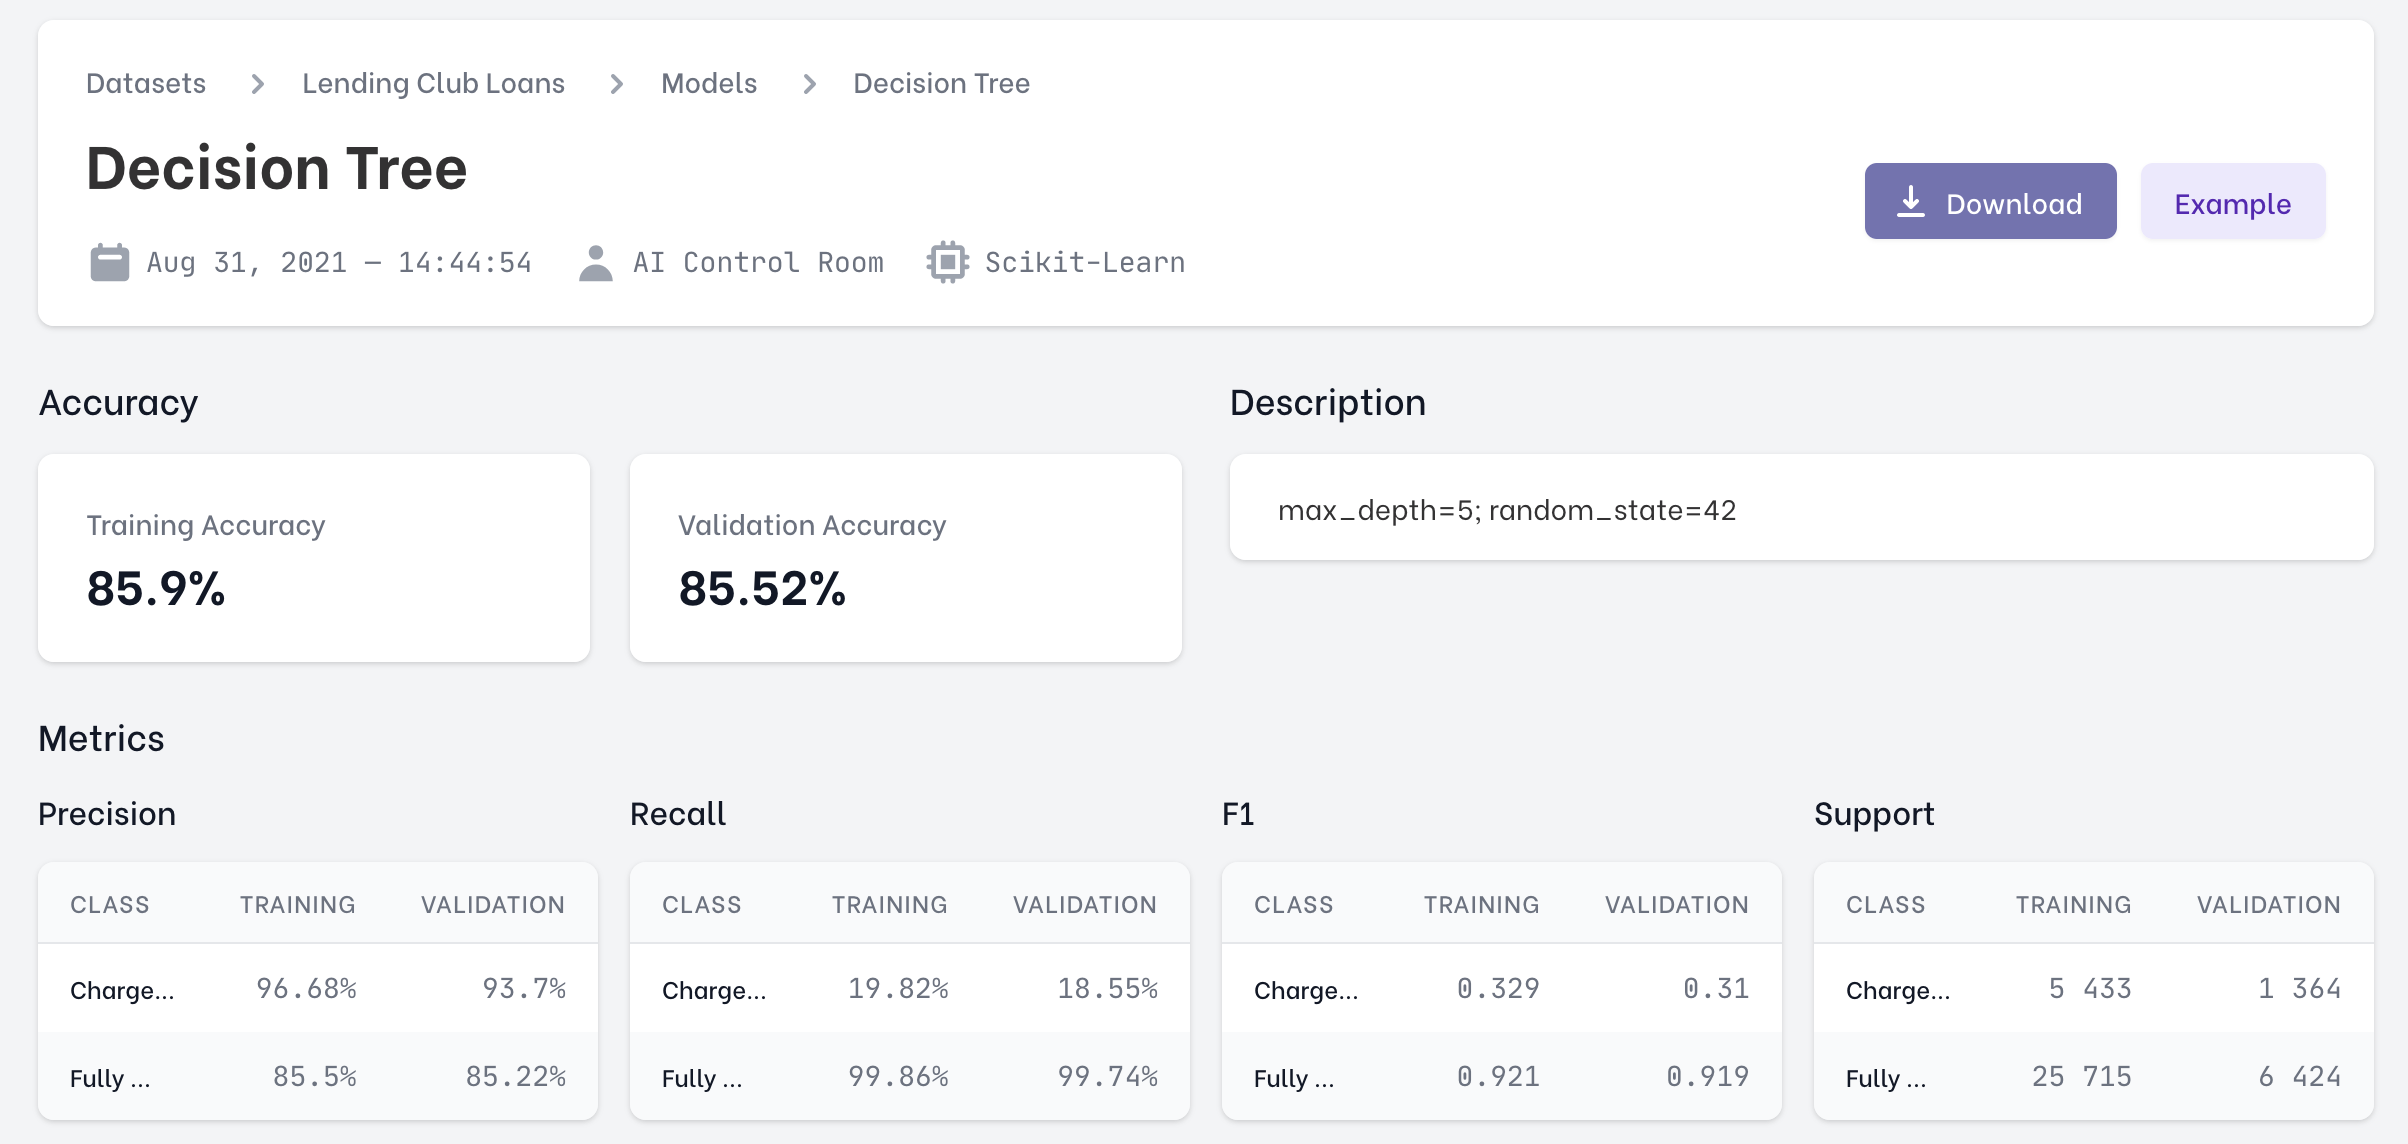
\includegraphics[width=\textwidth]{img/screenshots/model_assessment_overview.png}
    \caption{AI Control Room - Model Assessment Overview with Standard Metrics}
    \label{fig:model_assessment_overview}
\end{figure}
\begin{figure}[htbp]
    \centering
    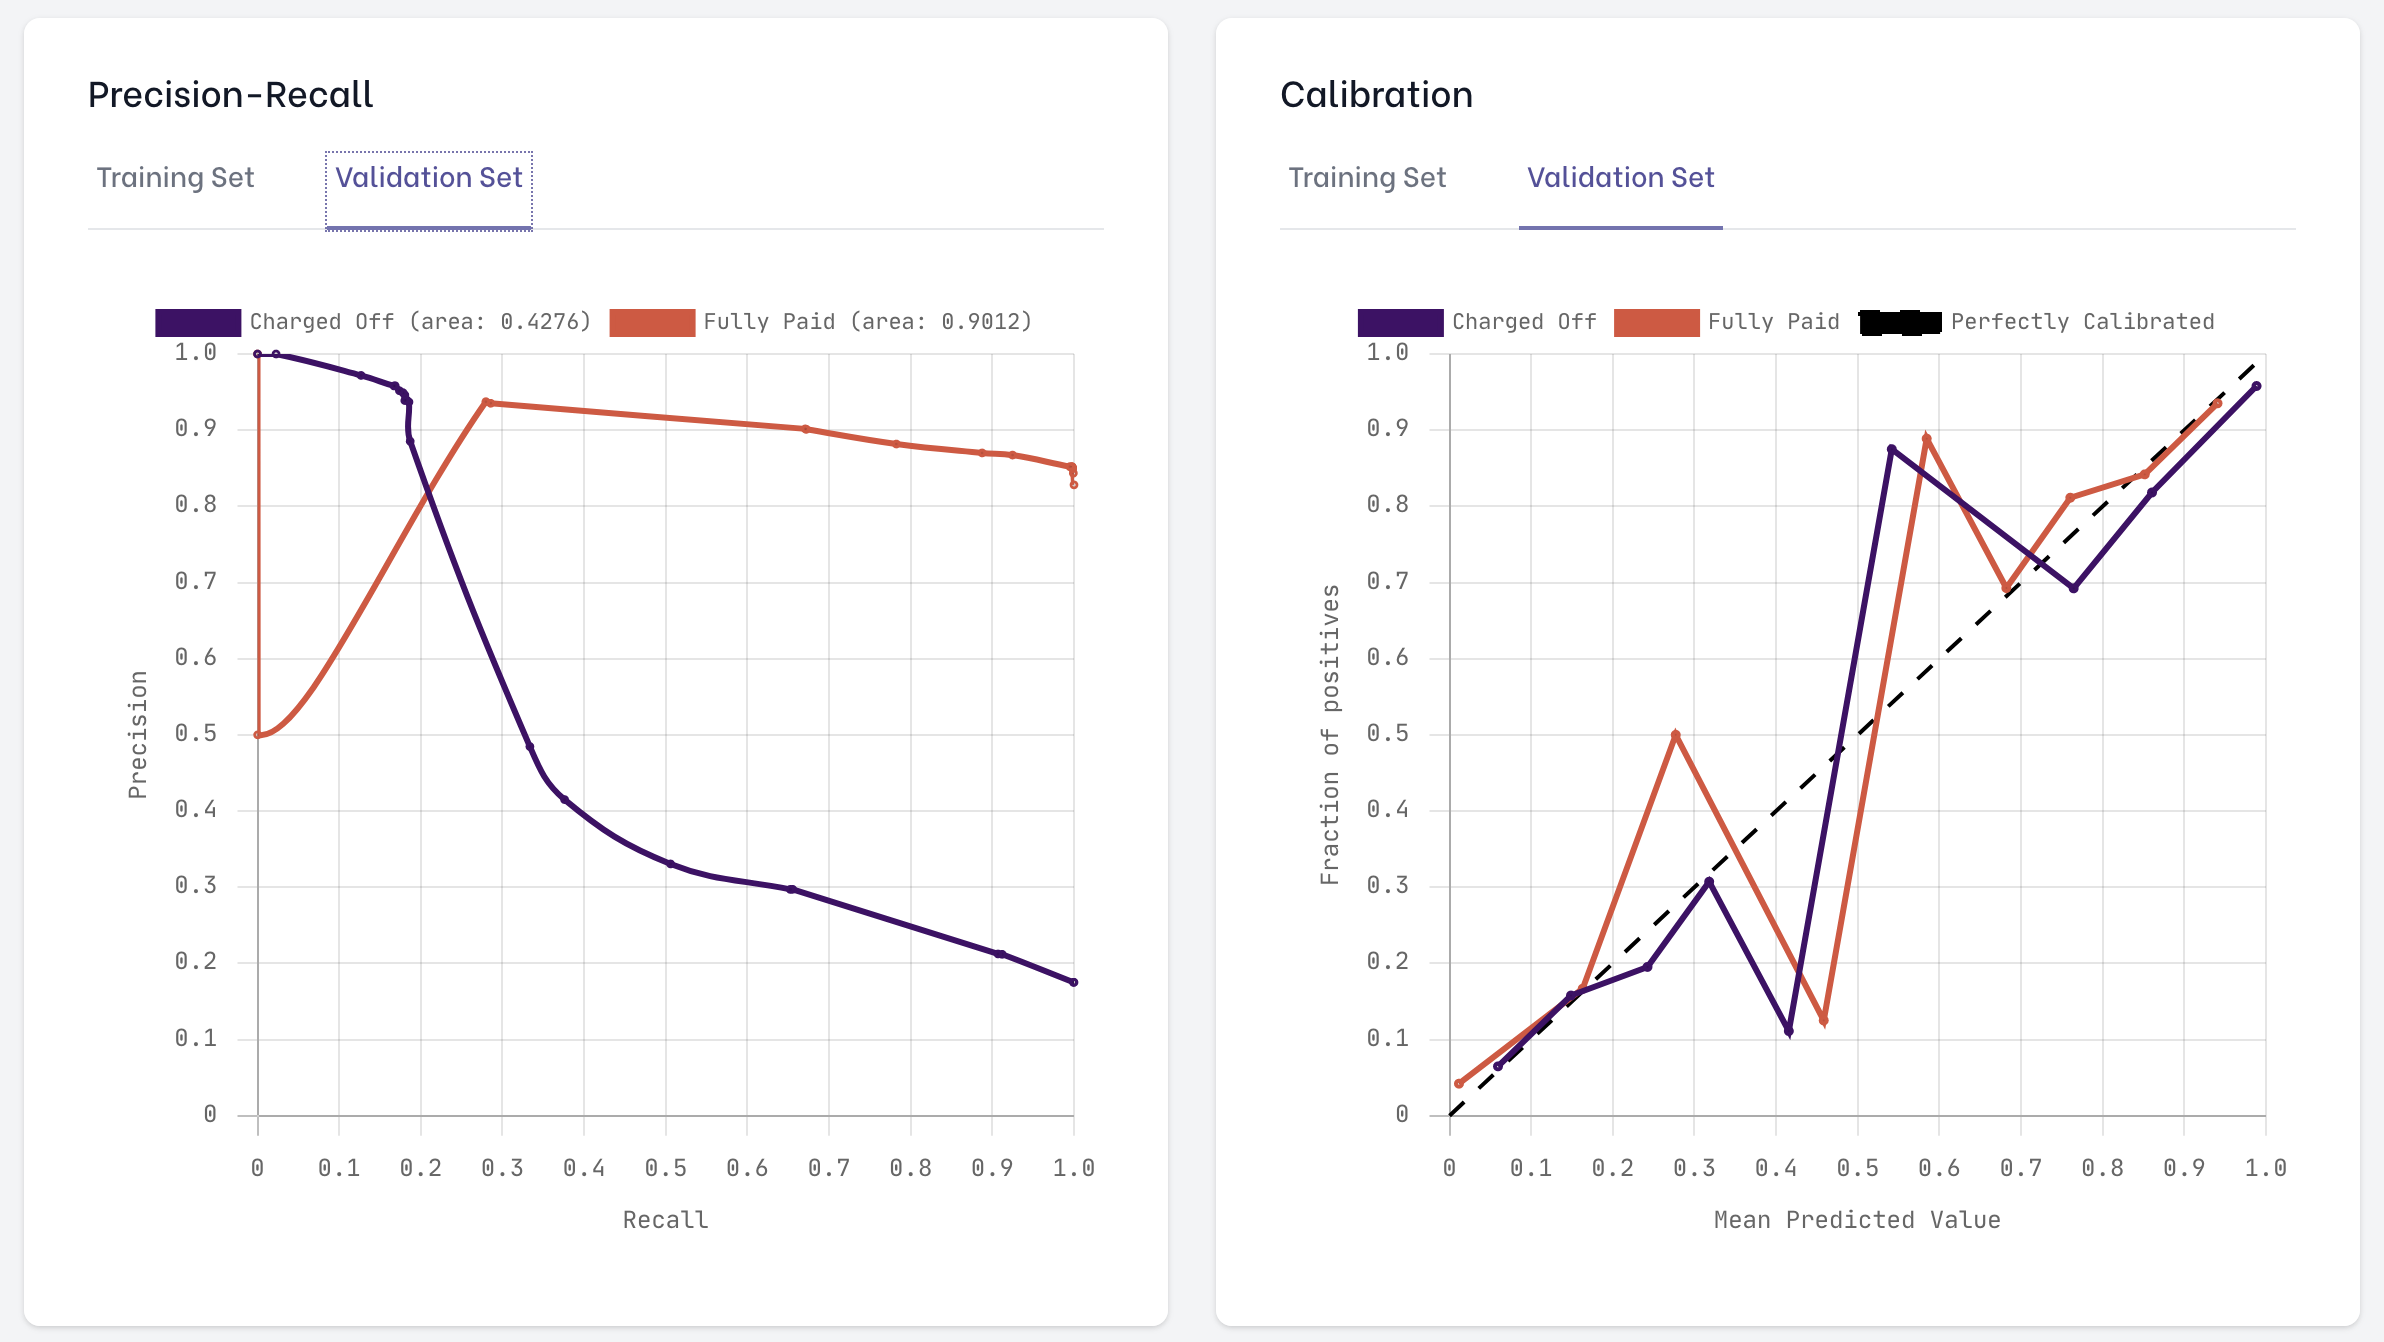
\includegraphics[width=\textwidth]{img/screenshots/model_assessment_graphs.png}
    \caption{AI Control Room - Precision-Recall and Calibration Graphs}
    \label{fig:model_assessment_graphs}
\end{figure}
\begin{figure}[htbp]
    \centering
    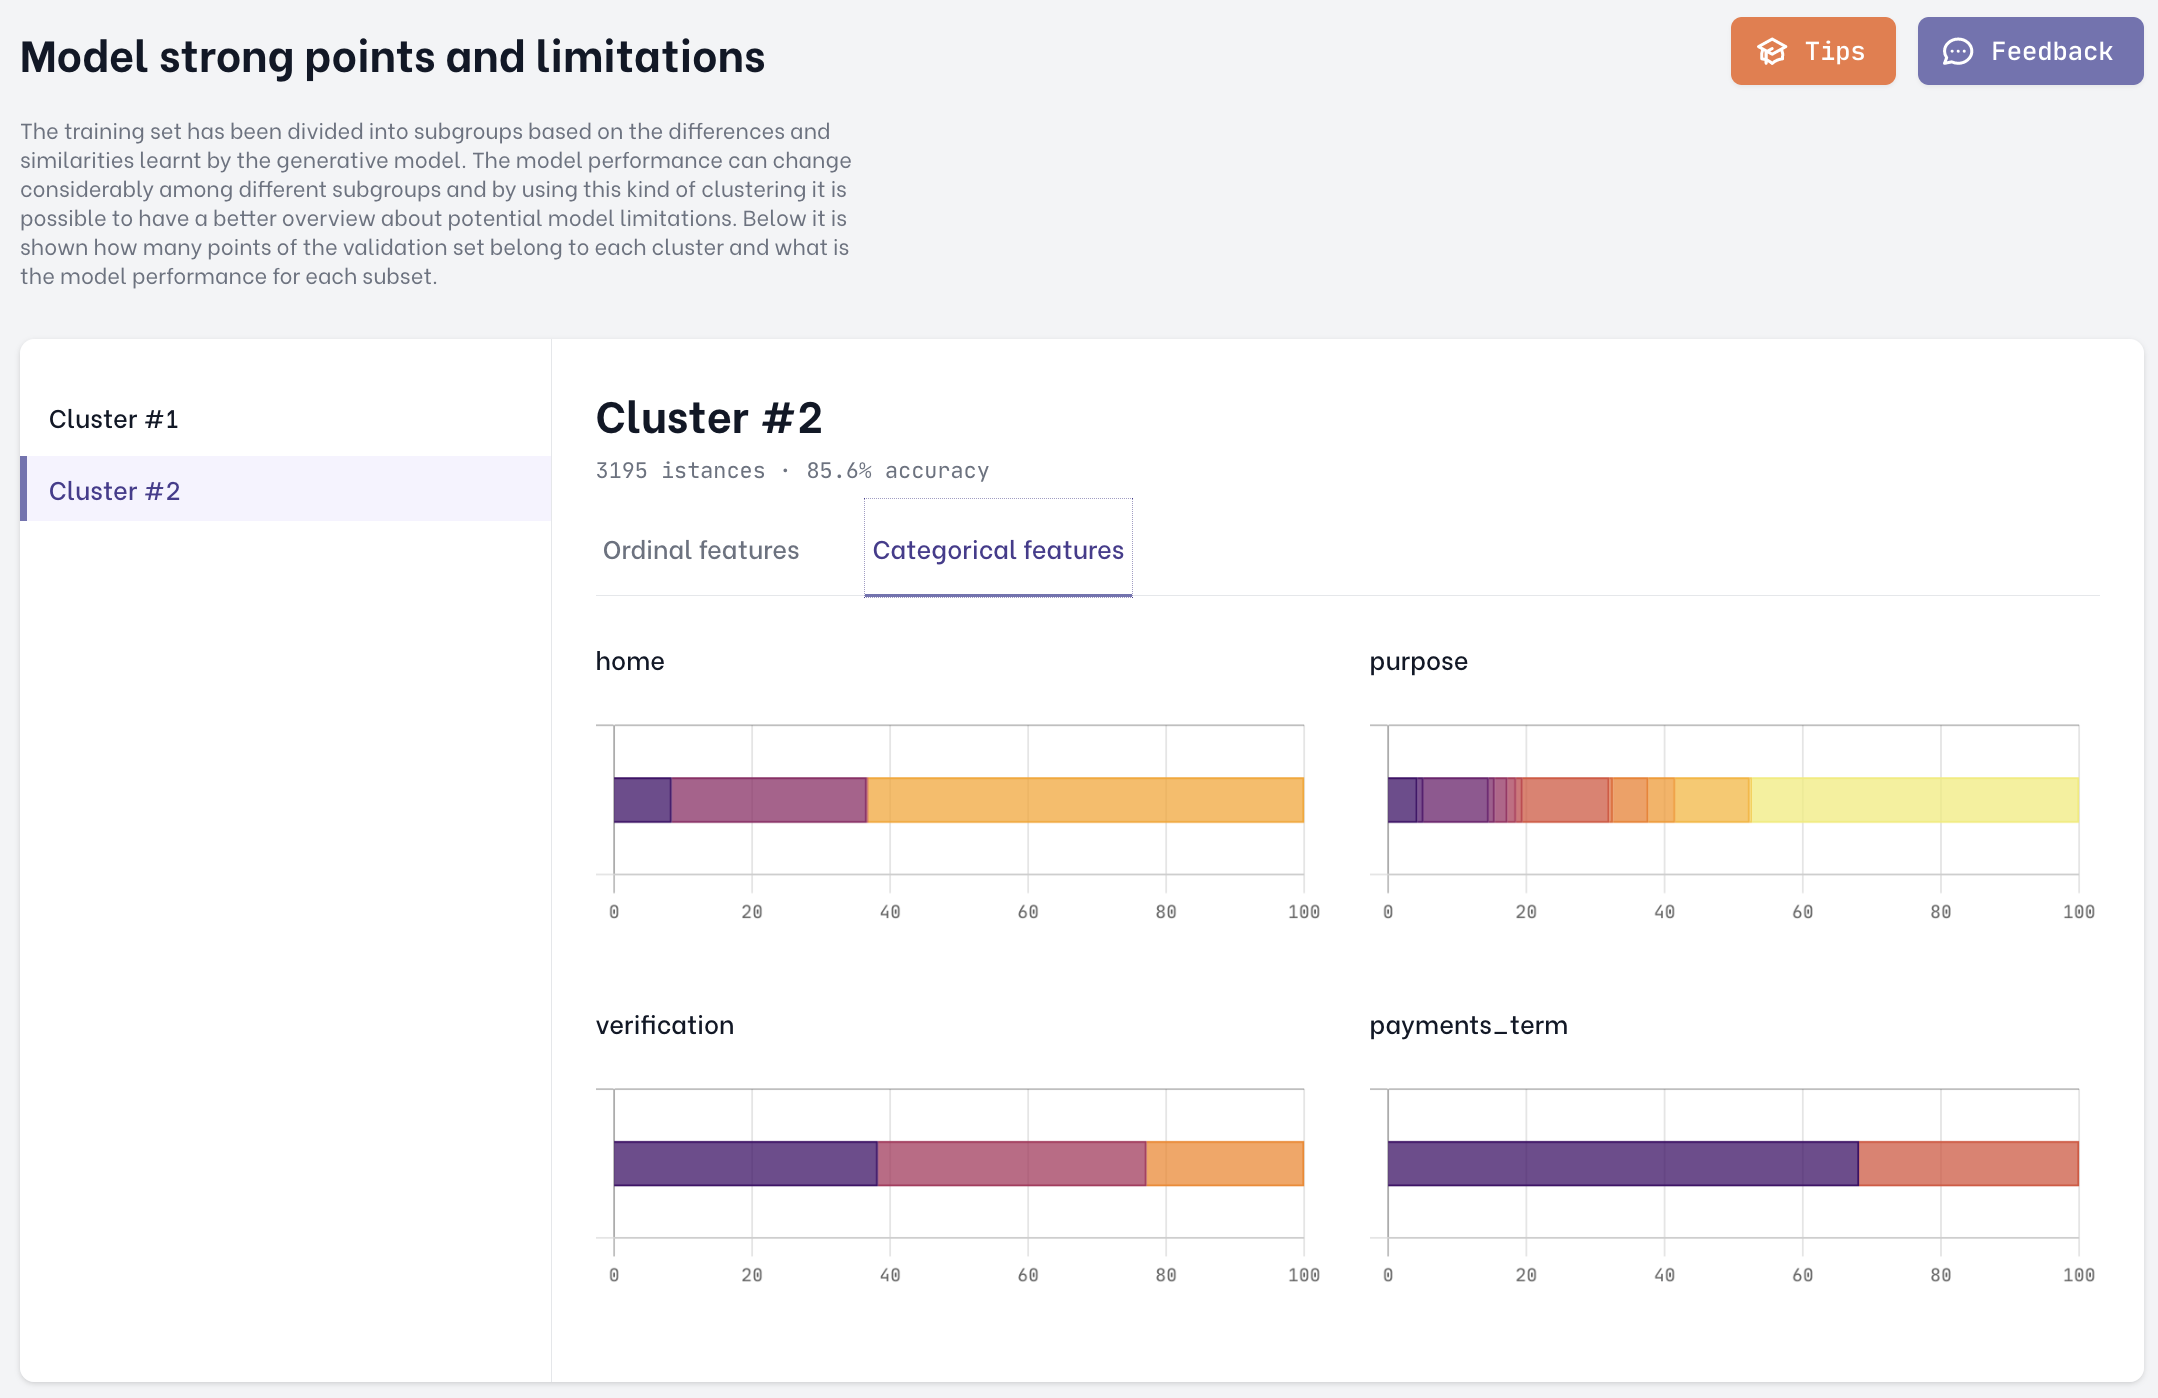
\includegraphics[width=\textwidth]{img/screenshots/model_assessment_analysis.png}
    \caption{AI Control Room - Model String Points and Limitations}
    \label{fig:model_assessment_analysis}
\end{figure}
\begin{figure}[htbp]
    \centering
    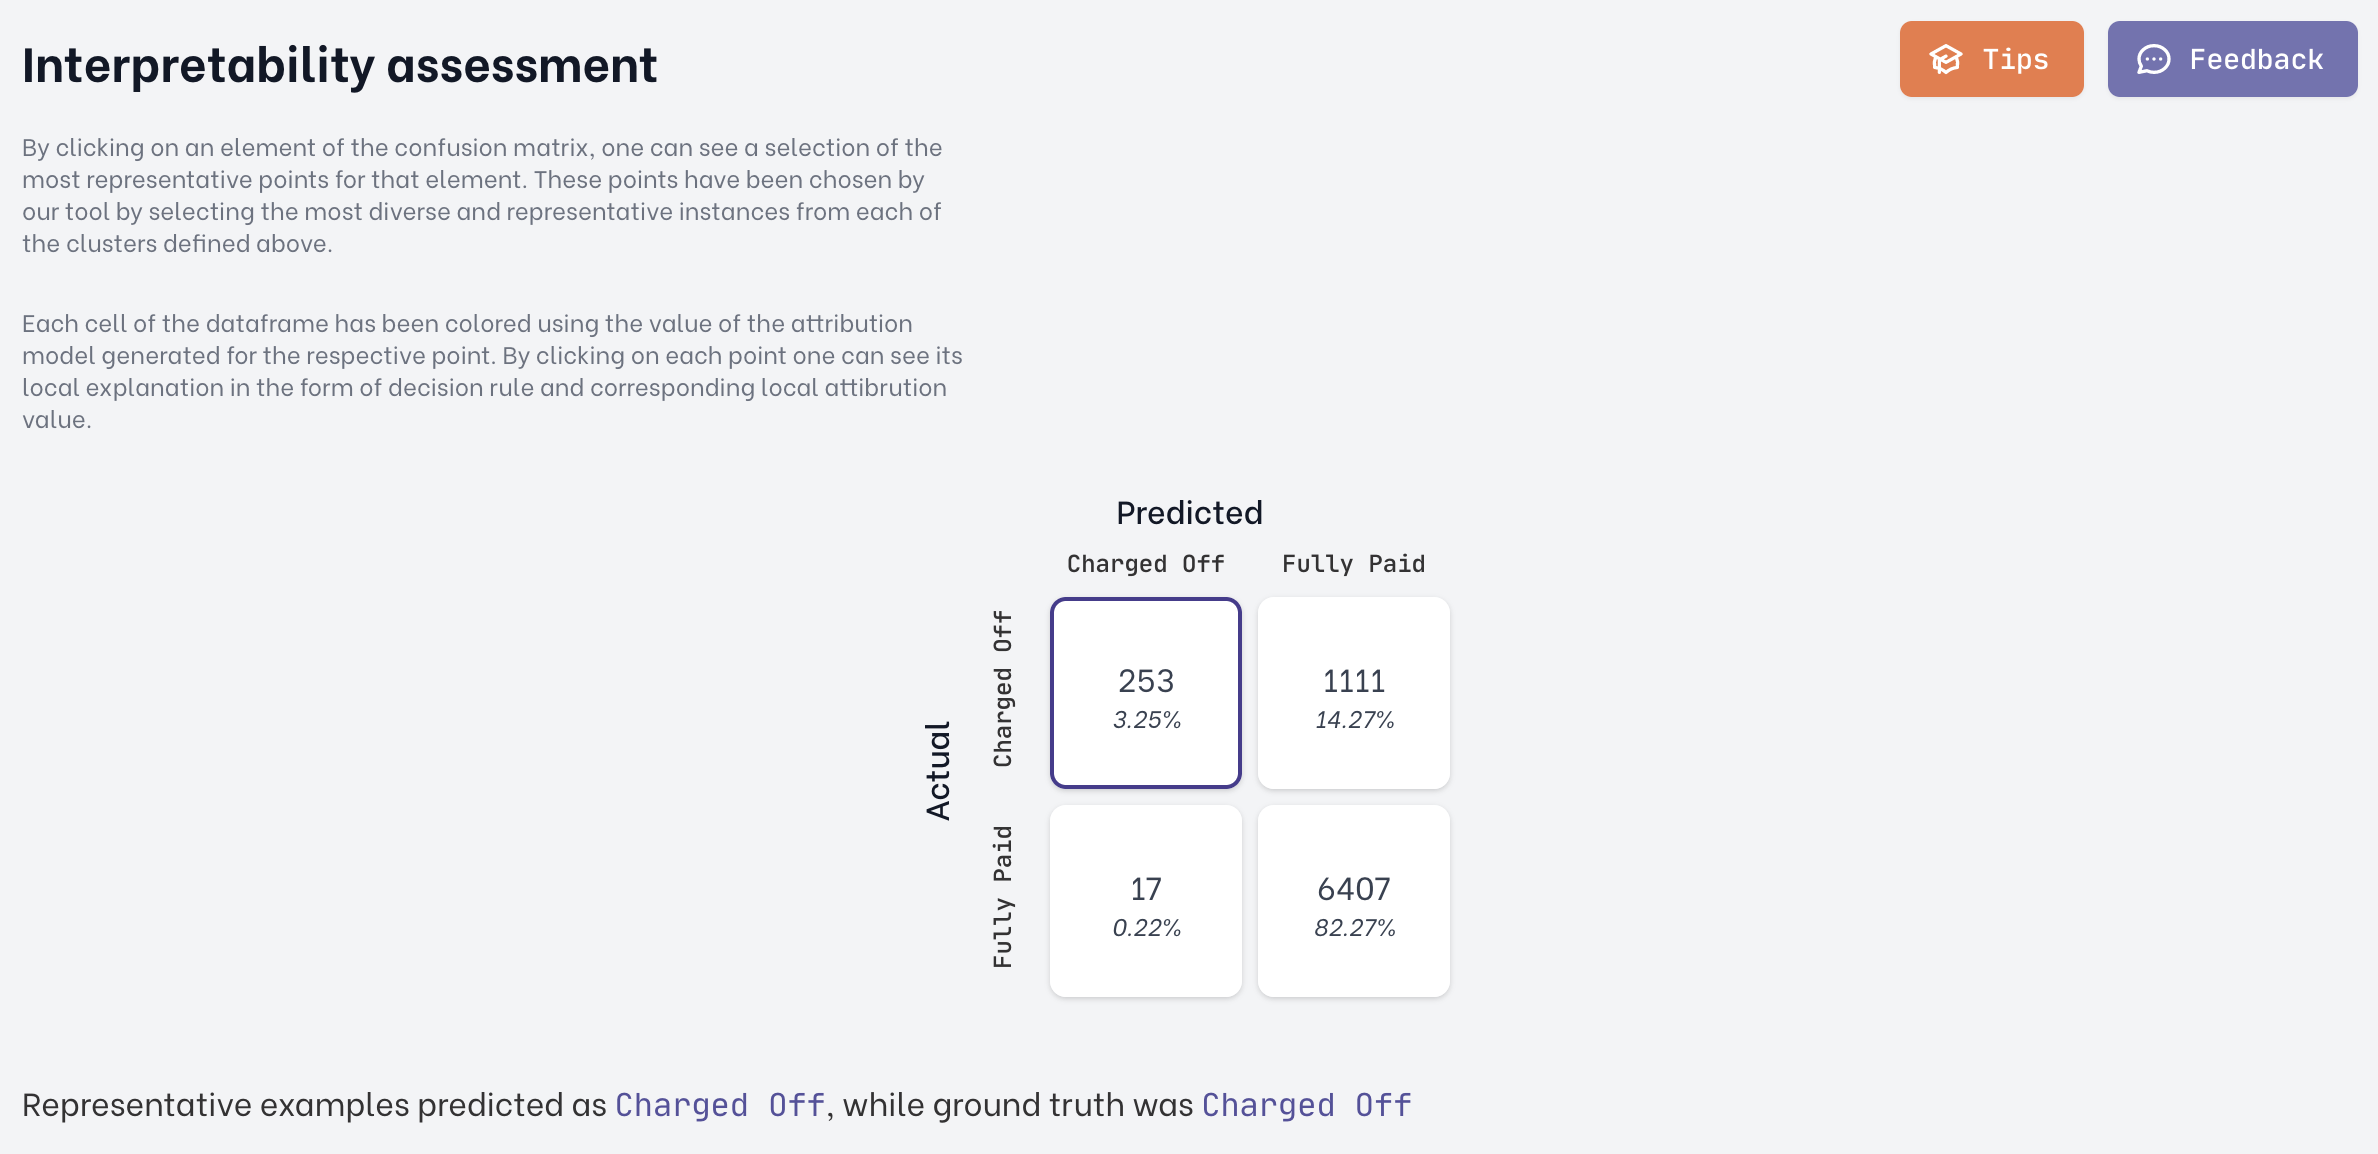
\includegraphics[width=\textwidth]{img/screenshots/model_assessment_interpret.png}
    \caption{AI Control Room - Interpretability Assessment}
    \label{fig:model_assessment_interpret}
\end{figure}
\begin{figure}[htbp]
    \centering
    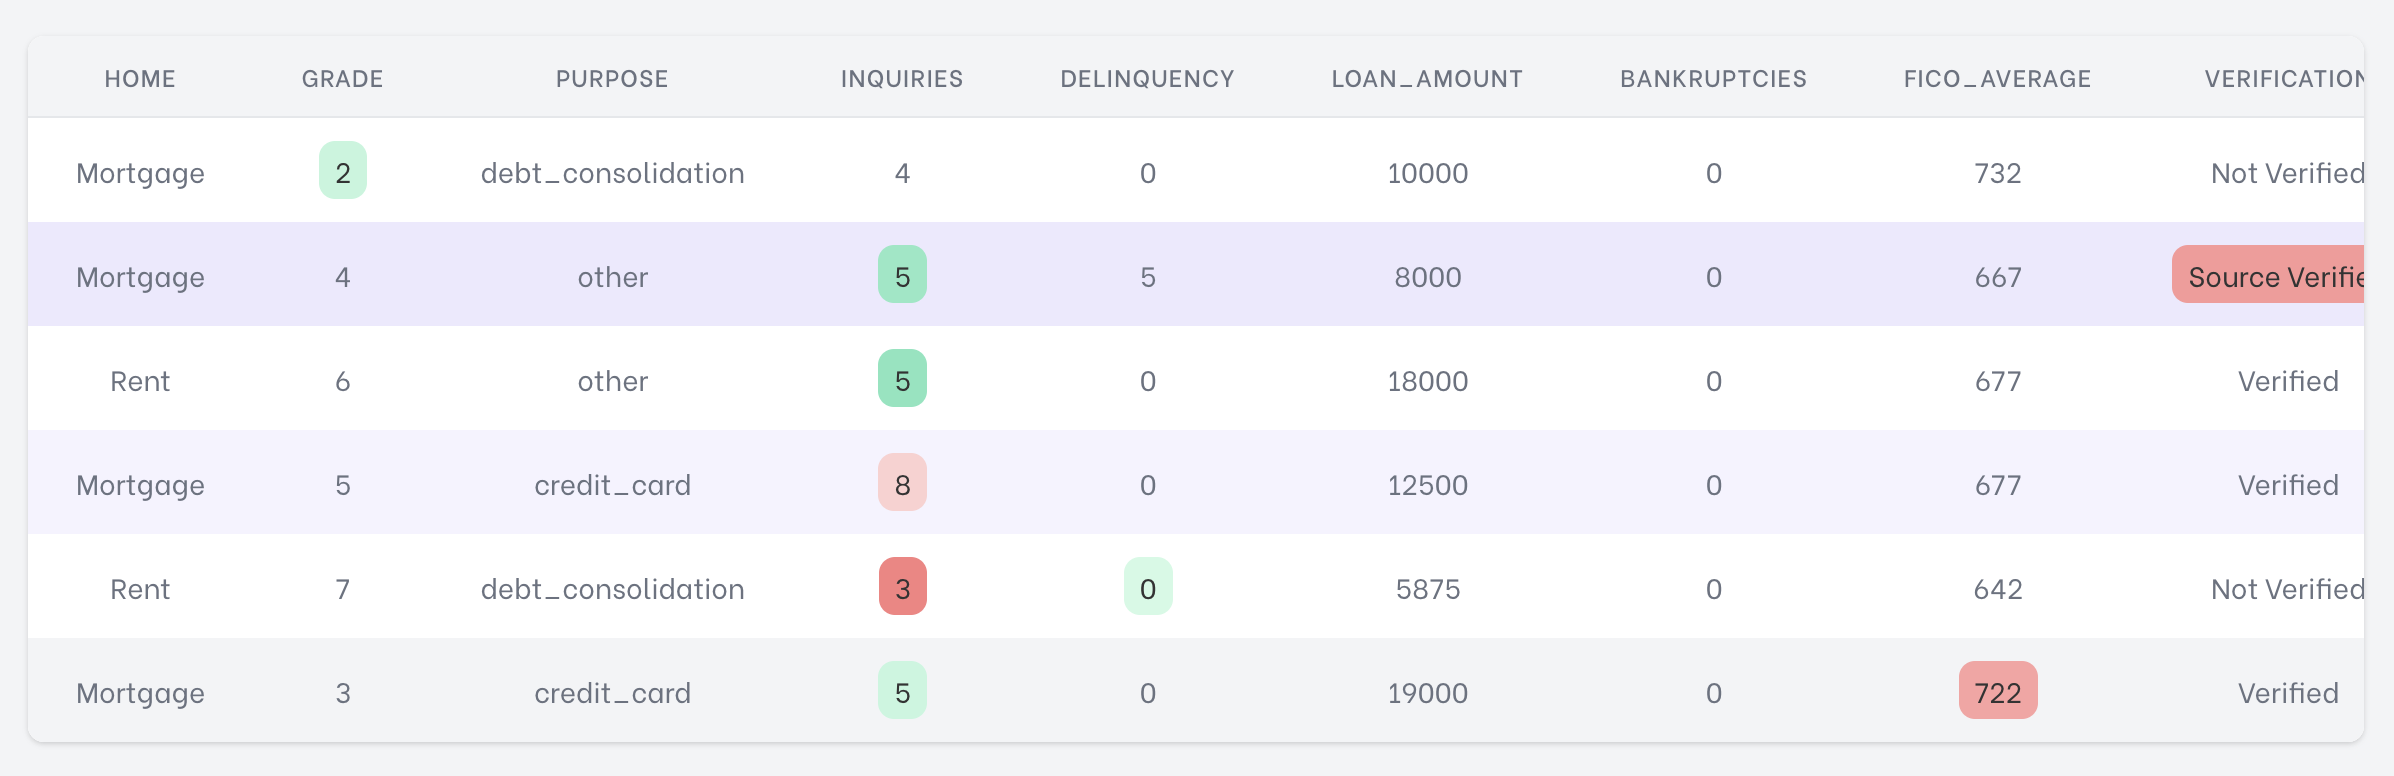
\includegraphics[width=\textwidth]{img/screenshots/model_assessment_examples.png}
    \caption{AI Control Room - Example Data}
    \label{fig:model_assessment_examples}
\end{figure}
\begin{figure}[htbp]
    \centering
    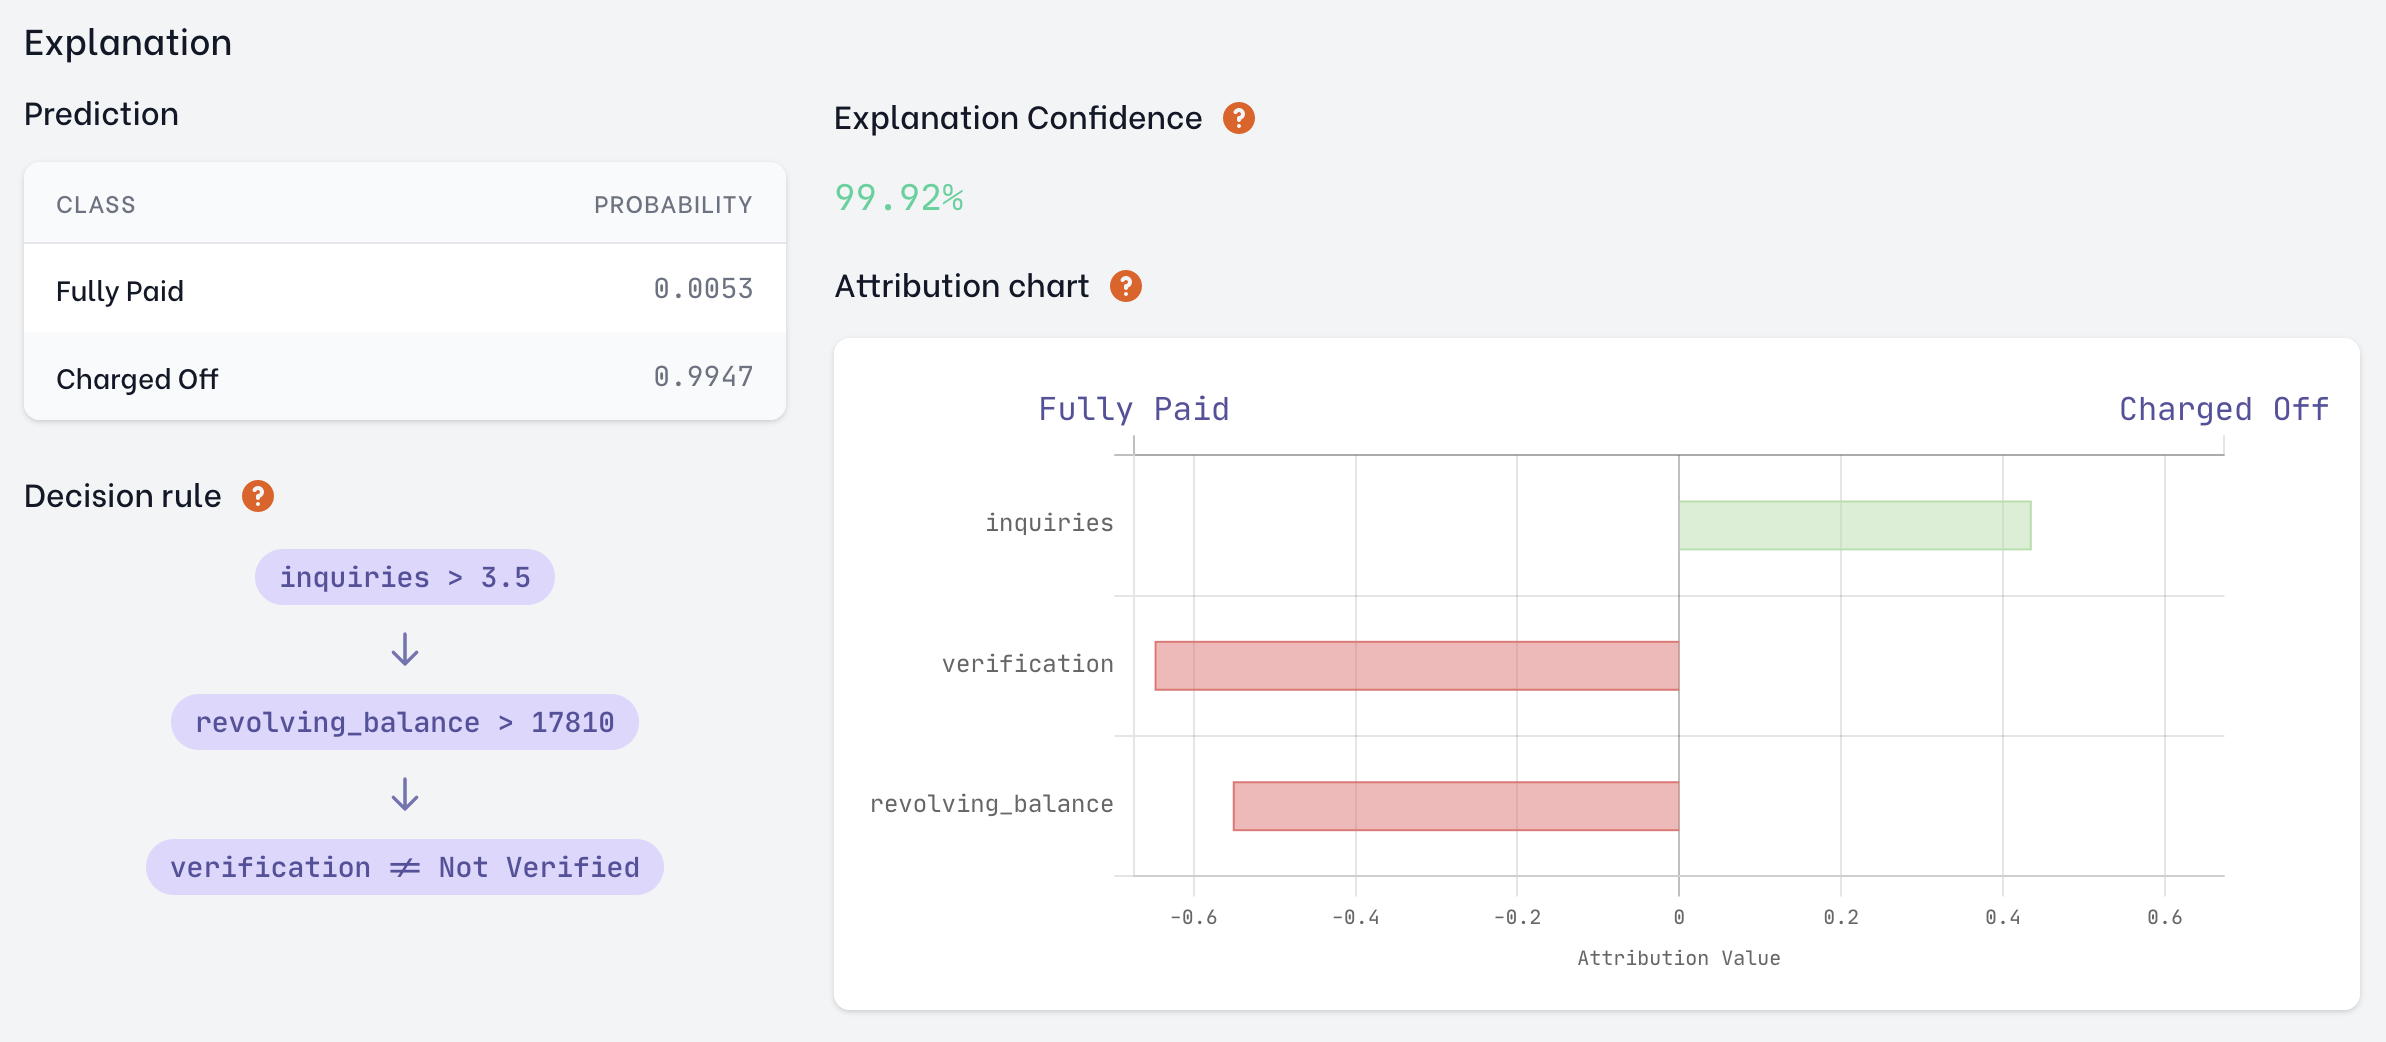
\includegraphics[width=\textwidth]{img/screenshots/model_assessment_explanation.png}
    \caption{AI Control Room - Prediction Explanation for Examples Data}
    \label{fig:model_assessment_explanation}
\end{figure}
\clearpage

\section{Approach}
As already described in the introduction of \autoref{chapter:introduction}, many machine learning algorithms score high on standard performance metrics, but user-facing performance may be way worse \parencite{gordon_disagreement_2021}. This issue is caused by real world applications being very dependent on the actual human-AI-interaction. Following this reasoning, it lends itself to utilize a human-centered design process for creating AI assessment systems. \autoref{fig:DIN_EN_ISO_9241} shows a standardized process of human-centered design, which was applied in this thesis to conceptualize, implement and evaluate assessment system artifacts. The key take-away is the inclusion of human aspects in all stages of the process. Research on evaluation of AI explanations revealed that there is a big gap between the perceived and actual usefulness of explanations, as described by \textcite{ras_explainable_2021}. This further underlines the need for a human-centered approach in designing AI assessment systems.

The thesis' structure will reflect the human-centered approach, which is visualized in \autoref{fig:DIN_EN_ISO_9241}: As already alluded in \autoref{chapter:introduction}, \autoref{chapter:analysis} is about understanding and setting the context of use by conducting literature research and user interviews. Based on the established requirements \autoref{chapter:conception} will describe the conception of functionalities and interaction design. The development of solutions will be described in \autoref{chapter:implementation}, while \autoref{chapter:evaluation} is about the evaluation of the solutions. This general process is embedded in a iterative loop, where intermediate results are evaluated against the requirements and subject to change.
\begin{figure}[htbp]
    \centering
    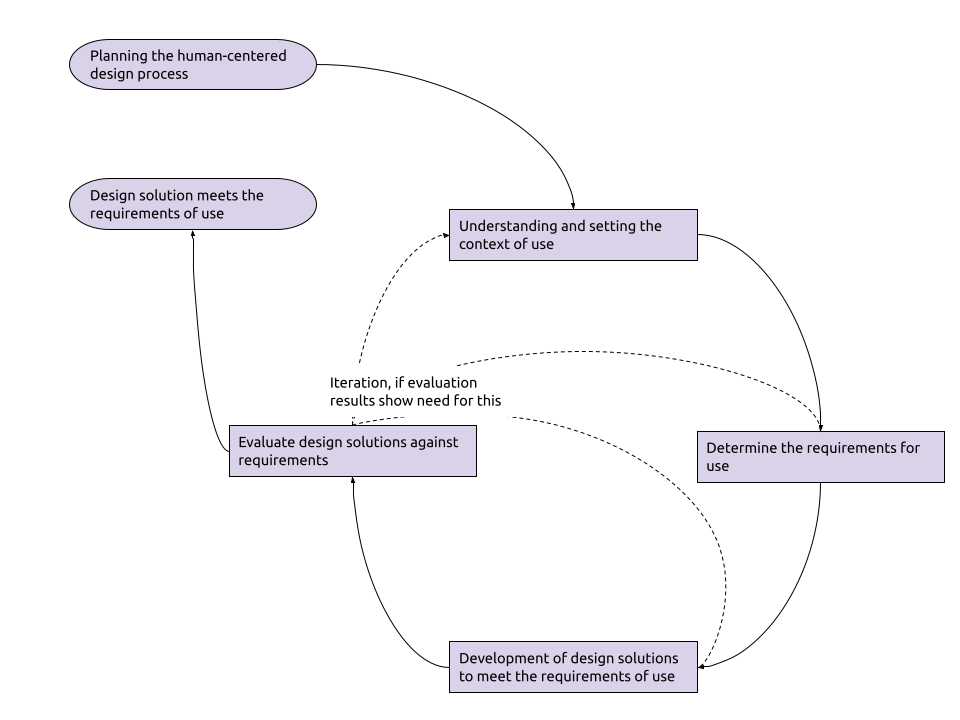
\includegraphics[width=\textwidth]{img/figures/DIN_EN_ISO_9241-210.png}
    \caption{Human-centered Design Process \parencite{DIN}}
    \label{fig:DIN_EN_ISO_9241}
\end{figure}

\newpage
\chapter{Analysis}\label{chapter:analysis}
Following the human-centered design process, it is important to incorporate the potential users from the beginning \parencite{harte_human-centered_2017}. This is also reflected in the analysis, where the context and setting of use has to be understood and set. Besides the human factors, there are also more general and theoretical aspects to be analysed, such as the context of AI in the medical application domain for specific tasks, such as classifying disease patterns with medical imaging.

In the following the context, task, problem and users will be described and analysed as a foundation for the human-centered design process and the following conception of AI assessment system artifacts.

\section{Data Sources}
Three main data sources where used for the analysis, ranging from general scientific literature about XAI to expert interviews and cooperation with developers of an existing application.

\subsection{Scientific Literature}\label{subsection:literature}
As described by \textcite{mueller_explanation_2019}, the amount of scientific publications on the topic of explanation in intelligent systems has surged in the last 5 years, revealing many important and relevant information on this subject area through openly accessible papers. In the beginning of the thesis (July 2021) a general search on \textit{Google Scholar} was conducted to gain a overview on available publications. A non-exhaustive list of search terms at the time was:
\begin{itemize}
    \item XAI
    \item XAI in Medical Applications
    \item Explainable Artificial Intelligence
    \item Explainable Artificial Intelligence in Medical Applications
    \item Explainable Machine Learning
    \item Interpretable Machine Learning
    \item Explaining Black-Box Machine Learning Models
    \item Explaining DNNs
\end{itemize}
This general research yielded already good results, as there were many relatively new and popular publications on the topic of XAI, such as \textcite{mueller_explanation_2019,ras_explainable_2021,ras_explanation_2018,adadi_blackbox_2018,hoffman_metrics_2019}, dealing with (1) issues of black box models (2) trustworthiness and transparency of AI-based systems (3) challenges of AI explanations (4) synopsis of key ideas of XAI (5) compilation of existing XAI methods among other topics.

The results of the internet research were then further reinforced by academic partners from the University of Lübeck, with whom related research was conducted in the context of the \textit{CoCoAI} project. Additional important scientific papers for the analysis were: \textcite{arrieta_explainable_2019,knapic_explainable_2021,samek_explaining_2021}, dealing with (1) review of AI explanation methods (2) XAI methods for decision-support in medical image analysis scenarios (3) literature analysis of XAI publications.

The literature research resulted in a foundation on the XAI topic with a thematic focus on black box image classifiers, available explanation methods and trustworthiness of AI applications. While many of the presented publications discuss theoretical and technical aspects of XAI, human-centered perspectives were found to be rare. \textcite{samek_explaining_2021} for example gives a detailed theoretical and technical overview of many explanation methods, but reduces the human interpretability of visual  explanations to only the file size, concluding that lower file sizes are more interpretable to the user. Furthermore \textcite{ras_explainable_2021} presents many ways to objectively compare explanation methods, but also highlights the difficulties of user-centered explanations, tailored to specific requirements such as medical professionals have for decision support systems. However there is also literature on psychometric evaluation of XAI systems \parencite{hoffman_metrics_2019} with a strong focus on human aspects. Overall the literature research showed that the XAI domain heavily focuses on the theoretical, technical and organizational aspects of explanation methods, while only very few authors consider user-centered research methods from the HCI domain, which also found by \textcite{mueller_explanation_2019}.

\subsection{Interviews}\label{subsection:interviews}
Complementing the general research on XAI, expert interviews where conducted. These interviews specifically target medical professionals and data scientists. Interviews with the actual user group of a potential solution is key to understanding and setting the context and requirements of use. The participants for the interviews were chosen with following requirements in mind:

\begin{description}
    \item[Medical Professionals:] Has interest and/or knowledge in AI-systems; has worked with or researched AI-systems in the medical domain; can judge the benefits and risks of the use of AI in medical applications.
    \item[Data Scientists / AI Researchers:] Is familiar with the XAI topic; has interest in explainability and trustworthiness of machine learning models; has worked with AI in the medical context.
\end{description}

Participants for the interviews were gathered via academic partners, internet research and word of mouth. 16 suitable people from 6 different institutions were contacted about potential interviews. Ten leads were medical professionals while six leads where data scientists or AI researchers. In total, 4 interviews were conducted. The participants are described in further detail in \autoref{table:interview_participants}.

The Interviews were conducted in German and executed as one-to-one online interviews. The interviews were recorded for later reference if consent was present. Additionally the interviews were supported by a research colleague, who kept protocol. After the interviews the recordings were transcribed for further analysis and the participants were asked to answer the \textit{Affinity for AI Interaction} (\textbf{AAII}) questionnaire, which is a modified version of the \textit{Affinity for Technology Interaction} (\textbf{ATI}) questionnaire \parencite{franke_personal_2019}. ATI aims to determine the tendency to actively engage in intensive technology interaction, as a key personal resource for coping with technology. Analogously the AAII questionnaire aims to determine the tendency to actively engage in AI interaction. The ATI questionnaire was modified to focus on AI interaction for a better thematic fit, as it is important to estimate how the user likes to deal with AI.

In terms of content, the interviews for medical professionals and data scientists were slightly different as seen in \autoref{table:interview_topics}. The reason for this is the heterogenous expertise on the subject area of machine learning models and potential user requirements. The whole interview guideline can be found in \nameref{appendix:interview_guideline}.

\begin{table}[htbp]
    \centering
    \begin{tabularx}{\textwidth}{ l l l X X l }
        \toprule
        ID & Age & Gender & Occupation & Education Level & AAII Score \\
        \midrule
        1 & 28 & male & Assistant Physician in Neuroradiology & State Examination & 4.89 \\ 
        2 & 24 & female & Research Associate (ML) & Masters Degree & 5.12 \\ 
        3 & 48 & male & Surgeon & Dr. med. & 5.45 \\ 
        4 & 27 & female & Assistant Physician in Neuroradiology & State Examination & 4.67 \\ 
        \bottomrule
    \end{tabularx}
    \caption{Interview Participants}
    \label{table:interview_participants}
\end{table}

\begin{table}[htbp]
    \centering
    \begin{tabularx}{\textwidth}{ l l }
        \toprule
        Medical Professionals & Data Scientists / AI researchers \\
        \midrule
        Actual Usage of AI & Actual Usage of AI \\ 
        Perspective on AI Usage & Comparison of AI Models \\  
        Trust in AI & Perspective on AI Usage \\
        Potential Problems with AI Usage & Trust in AI \\
        Own Explanation Techniques & Potential Problems with AI Usage \\
        Familiarity with XAI & Own Explanation Techniques \\
        Assessment on Local Explanations & Familiarity with XAI \\
        Information Processing & Need for Local Explanations \\
        Reliability vs. Trust vs. Understanding & Need for Global Explanations \\
         & Information Processing \\
         & Trust-Behavior Connection \\
         & Reliability vs. Trust vs. Understanding \\
        \bottomrule
    \end{tabularx}
    \caption{Interview Topics}
    \label{table:interview_topics}
\end{table}

After gathering the interview data via protocols and transcripts a thematic analysis according to \textcite{braun_thematical_2006} was applied to identify common topics and codes. The thematic analysis is a widely used qualitative analysis method mainly found in the field of psychology and can be used as a primary tool to access data from interviews. Applying this method resulted in a thematic map showcasing common overlapping topics found in the interviews, which can be seen in \autoref{fig:thematic_mind_map}. The thematic map serves as the baseline for further context and requirement analysis.

\begin{figure}[htbp]
    \centering
    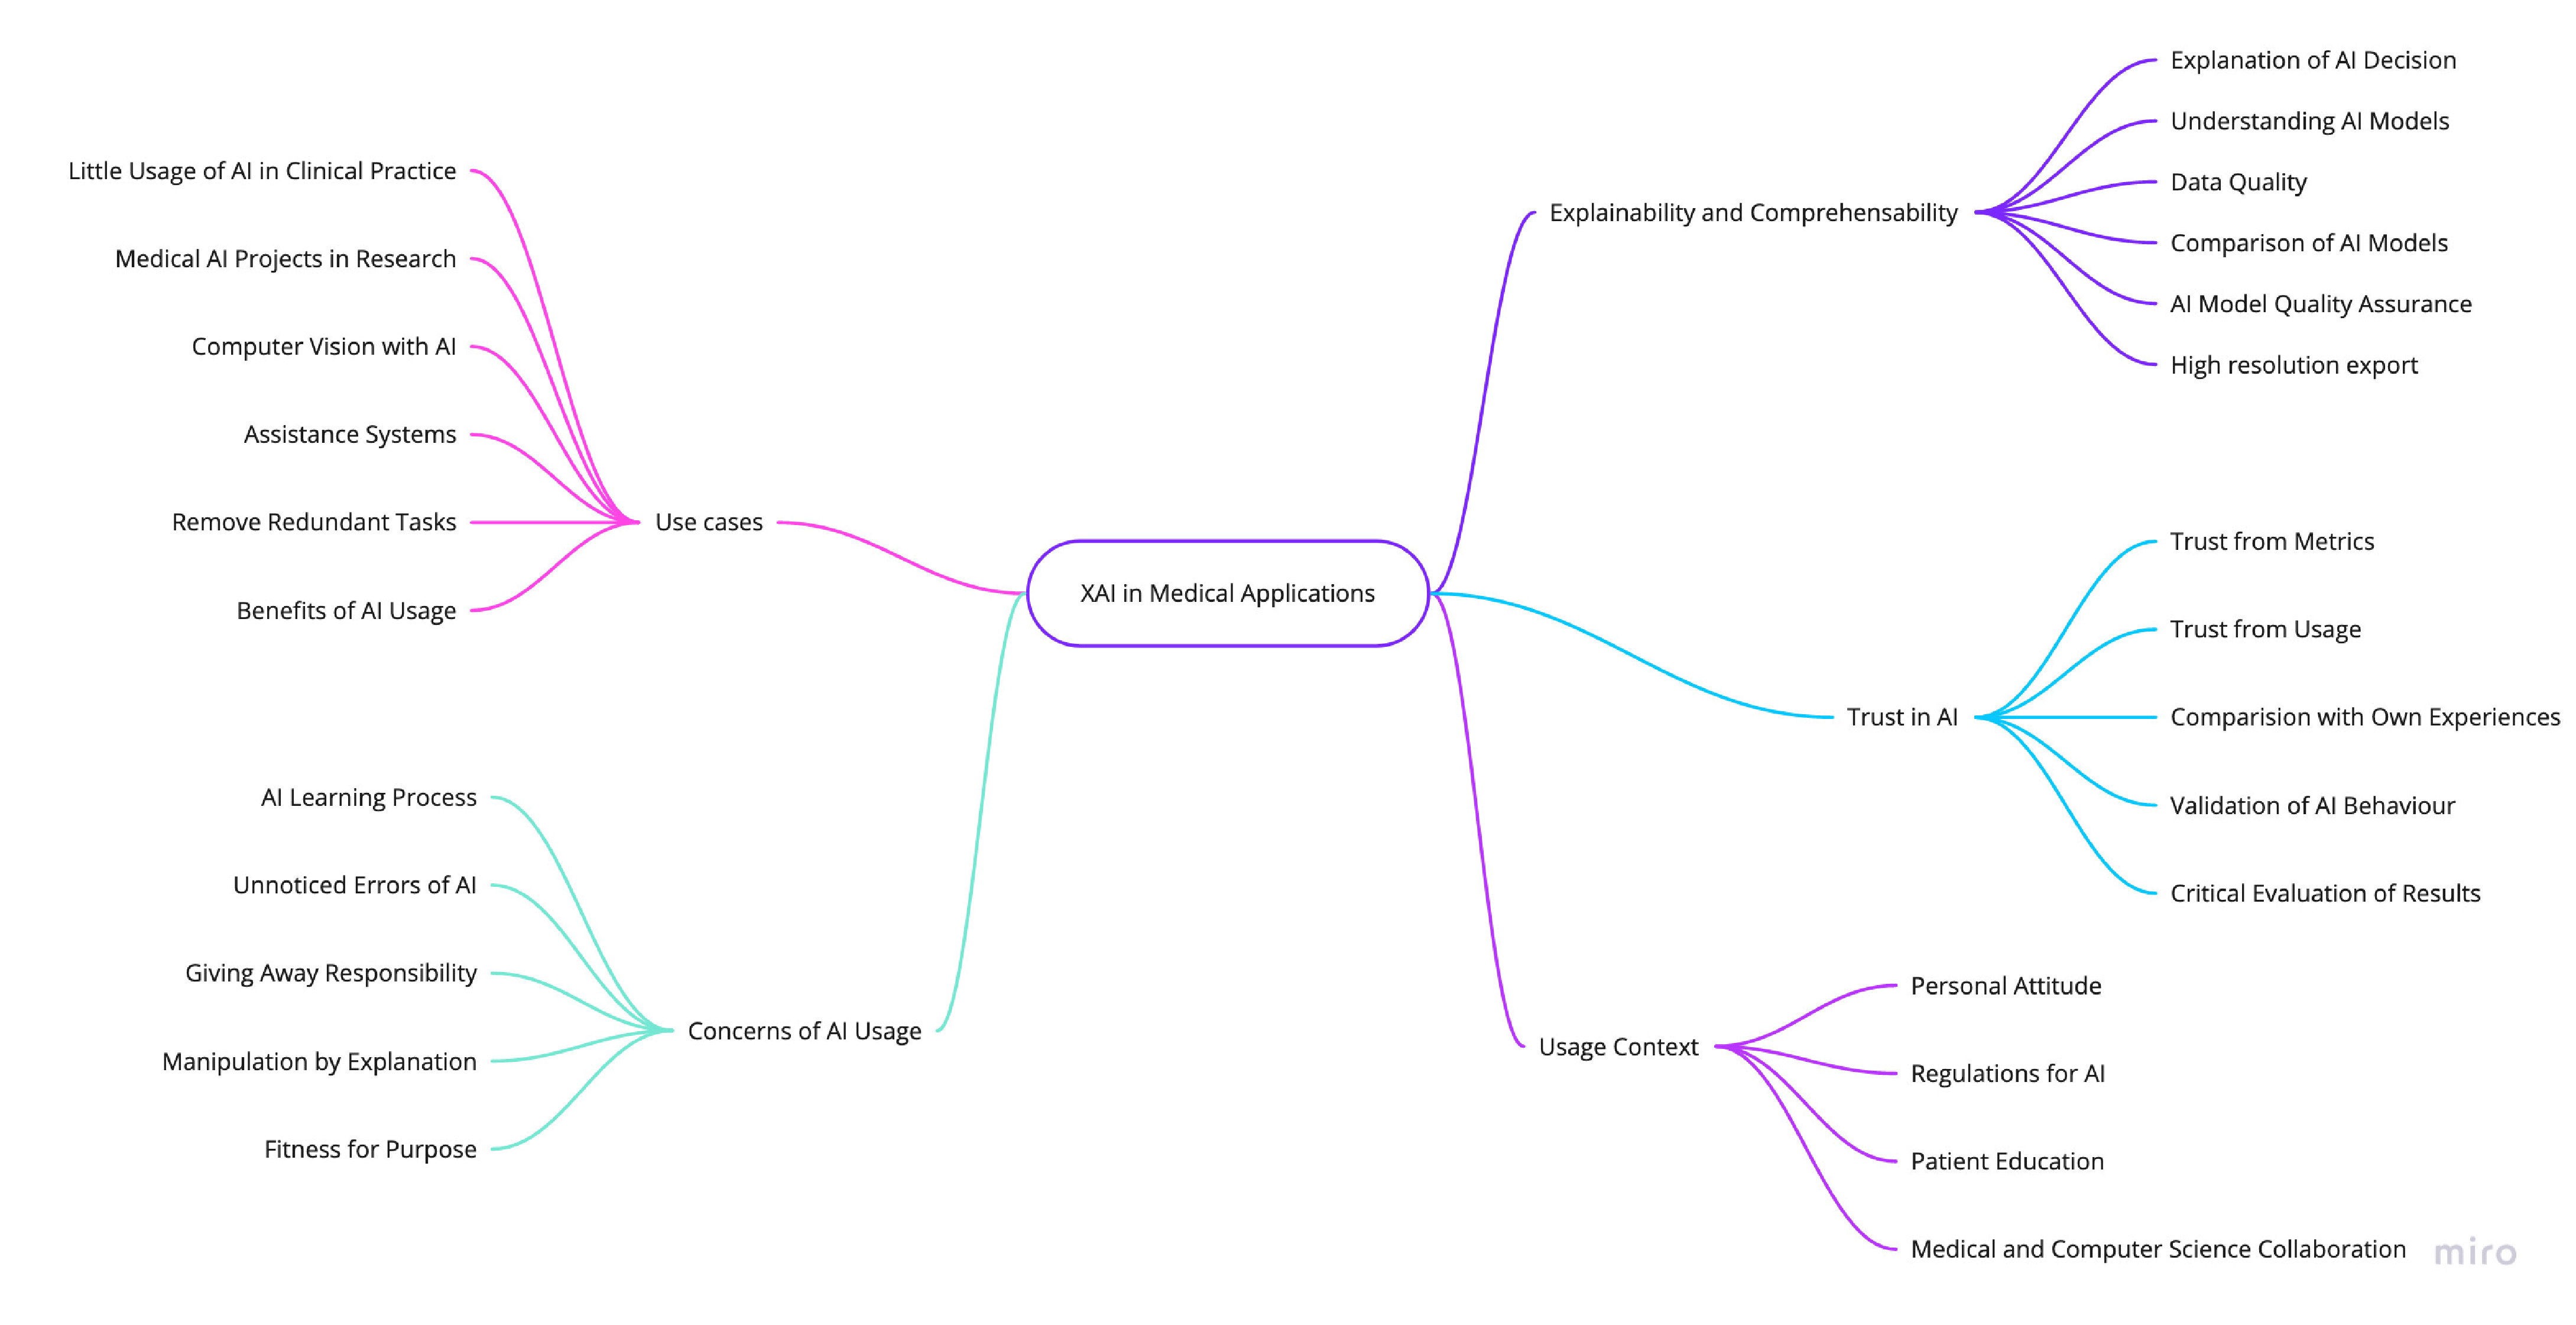
\includegraphics[height=0.8\textwidth, angle=90]{img/figures/Thematic_Mind_Map.pdf}
    \caption{Thematic Mind Map}
    \label{fig:thematic_mind_map}
\end{figure}

\subsection{Existing Applications}\label{subsection:existing_apps}
A scientific cooperation with Clearbox AI allowed us to access a additional source of information, valuable for the analysis and conception. As already described in \autoref{section:state_of_the_art} Clearbox developed an AI model assessment solution among other things. During the period of cooperation regular meetings were held with the CTO and other employees. These meetings were used for knowledge exchange on the subject of XAI literature, previous experiences, feedback and conceptional workshops. In particular, resources such as \textcite{people_ai_google_website,captum_website,streamlit_website} were valuable additions to the analysis. Furthermore the (beta) access to the Clearbox AI \textit{Control Room} cloud platform and the communication of user feedback was also used to gather information for the analysis and conception of an assessment system for image-based AI models.

\section{Context Analysis}
Black-box DNNs have become pervasive in todays society and represent a proven and indispensible machine learning tool. While these machine learning models can easily be used in recreational non-risky contexts, this does not hold true for the medical domain where decisions based on the results of a machine learning model can bear great risks for users and patients. This issue stems from the lack of interpretability and trustworthiness of DNNs \parencite{adadi_blackbox_2018}. DNNs architectures are inherently hard to understand and therefore interpretability of and trust in the results of such neural networks are a challenge.

Creating a solution to explain AI models a priori to the use can help setting the right expectations towards the AI model. Consequently the users of such a explanatory system gain the ability to build a fair mental model before using the AI, which in turn can support the formation of appropriate levels of trust \parencite{hoffman_metrics_2019}. This is beneficial to the user and facilitates efficient usage of the model in production \parencite{hoffman_metrics_2019, people_ai_google_website}.

Explaining the model a priori also enables the solution to build computationally complex explanations, which can depend on data sets of thousands of images. Supplying the user with explanations potentially based on the whole data set can also be beneficial: Statistical analysis and clustering of the data and metadata can support the understanding of model limitations and edge cases, while exemplary local explanations can be statistically distributed to gain a better overview of global behavior of the model. Combining different types of a priori explanations improve the coverage of the key attributes of explanations - explainability, feeling of satisfaction, sufficiency of detail, completeness, usefulness, accuracy, and trustworthiness - which were described by \textcite{hoffman_metrics_2019}.

The aspects mentioned above are also reflected in the interview data. The following list showcases with \textit{DeepL} \parencite{deepl} translated quotes from interview partners regarding the need for (a priori) explanations for AI models aimed at the medical domain:
\begin{displayquote}
    "I think you have to be critical and look at the results carefully - is the result at all plausible?"
\end{displayquote}
\begin{displayquote}
    "What is the information that is interesting for the system or that is decisive for the decisions? What information is rather irrelevant?"
\end{displayquote}
\begin{displayquote}
    "If the explanations for the model are based on any data that are meaningless from my clinical experience, such as a stroke being pinned down by bone shapes. That would shake my confidence in the machine, even though it might give reliable results."
\end{displayquote}
\begin{displayquote}
    "If, for example, there is an outlier data point in a specific case and you are not quite sure why it is like this or how you should interpret it, then something like this [local explanation] is great, so that you can understand why the result is like this or like this."
\end{displayquote}
\begin{displayquote}
    "I've always been interested in exactly how this works, how much training data it's based on, what's behind it, why the system decides the way it does."
\end{displayquote}
\begin{displayquote}
    "[...] and you might also learn what the machine pays attention to, which I personally could also pay attention to when I look at the picture. That would certainly strengthen my confidence in the application."
\end{displayquote}

Overall the interview partners expressed a strong need for explanation and validation of AI models in medical applications. This finding highlights the need for explanations for the users of medical AI, where they are able to explore the data and capabilities of the AI model and therefore build appropriate levels of understanding and trust. Furthermore the medical professionals homogeneously stated a need for validation of the AI model's results with their own expertise prior to the clinical usage of the AI. Therefore an interactive a priori explanation tool implemented in a sandbox environment could satisfy the needs expressed by the professional users for their usage context.

\section{Problem and Task Analysis}
The following problem scenario summarizes the starting point of the problem and task analysis: The general medical practitioner Dr. med. Mustermann wants to offer thrombosis diagnosis in his office. He is not specialized in vein examination and thus has just basic knowledge and also no necessary equipment. In the past this has lead to him referring patients with venous disorders to a specialized clinic. Through a colleague he was made aware of "\textit{AutoDVT}", a AI based software developed by ThinkSono, which can help him offer DVT diagnosis in his office \parencite{thinksono_website}. The AutoDVT system works with image-based machine learning and can support medical professionals in real time with identifying DVT. Since Dr. med. Mustermann has very little knowledge of AI and machine learning he is very skeptical towards this innovative but foreign software system. Although he sees the immediate benefits of using a system which supports him with the examination of DVT, his trust in the system's predictions is very low and he fears relying on the AI's assessment. AI based technology is a black box for him, which he does not fully understand. The predictions of the systems are opaque to him and thus lead to rejection of the system.

DNNs for image classification are able to detect various disease patterns with medical imaging and can be used by medical professionals to support diagnosis and possibly increase efficiency and effectivity if trusted and used correctly \parencite{adadi_blackbox_2018,knapic_explainable_2021}. However, the reality looks different: Medical professionals bear the responsibility for their decisions regarding the patient and thus are rather relucant about using AI based systems - even though the AI could outperform them in image classification tasks. Most of the time decisions are based on personal experience, which was developed over a long period of time. This sentiment is reflected in the interview statements of medical professionals:
\begin{displayquote}
    "One risk, I believe, is also that you hand over responsibility to the machine."
\end{displayquote}
\begin{displayquote}
    "The classic risk of simply relying on what the algorithm says."
\end{displayquote}
\begin{displayquote}
    "The doctor with his expert knowledge will always compare this with his knowledge and experience, is this correct, what is the probability, is this in the range?"
\end{displayquote}

Modern DNN based image classificators, such as the \texttt{XRV\--DenseNet121\--densenet121\--res224\--all} model from \textcite{cohen_limits_2020}, can provide very good results in the prediction of pathologies. For example, the prediction accuracy for pneumonia is benchmarked as 86\% \parencite{torchxrayvision_github}. The use of such model or comparitive ones could benefit medical professionals in many ways as described by the interview partners:
\begin{displayquote}
    "It [AI system] facilitates standardized findings in particular"
\end{displayquote}
\begin{displayquote}
    "It [AI system] might give you a little peace of mind that you haven't missed anything."
\end{displayquote}
\begin{displayquote}
    "I always think to myself that this is based on CT gray levels, i.e. on these density values, and I always think to myself that it makes sense that a computer can distinguish these density levels better than my eyes."
\end{displayquote}

The benefits of using a DNN based image classificator to support medical professionals in detection and diagnosis of diseases are clear. For users to leverage these benefits trust in such a system must be given, which cannot be generated by mere accuracy metrics \parencite{samek_explaining_2021}. To overcome the hesitation of using AI in medical applications, a AI assessment system can be used to facilitate understanding of and trust in the algorithms. Stakeholders, such as practitioners or clinic managements, can use such a system to gain customized insights into the model and data prior to using it in everyday clinical practice.

\section{User Analysis}\label{section:user_analysis}
AI explainability and trustworthiness must be considered with respect to the individual who is regarded as the beneficiary of the explanation \parencite{mueller_explanation_2019}. For an assessment system that aims to explain AI models in the medical domain those user groups are: (1) Medical professionals, such as practitioners and clinic managements and (2) data scientists and AI researchers developing AI models. Naturally those two groups differ greatly from each other. While medical professionals have great expertise in various fields of examination, diagnosis and communication of pathologies, they also are expected to have little knowledge in computer sciences and machine learning. Data scientists on the other hand do have great knowledge of computer sciences, machine learning and neural network architectures, but lack the concrete medical expertise. Following the human-centered process the needs, requirements and whishes in regard to an AI assessment system of those user groups were analysed, mainly referencing the interviews from \autoref{subsection:interviews} and the resulting thematic map (see \autoref{fig:thematic_mind_map}).

\subsection{Medical professionals}
Through the interviews it was found that the surveyed participants differed in their experience and disposition towards AI systems. Surveying practitioners of different ages showed, that especially the younger ones, working in neuroradiology, are open towards using AI in their daily routine or that they are already using it. Some participants, took special courses on machine learning in the medical domain during their studies. Then again older, more experienced participants stated much less contact with AI in clinical practice. All interviewed medical professionals showed interest in medical AI in research projects and were positive on the benefits of AI, especially computer vision tasks. The most cited benefits were (1) great ability of machine learning to identify pathologies in medical images (2) take over of redundant tasks (3) backup for diagnosis and the handling of computationally expensive tasks. The medical professionals were also wary and timid about using AI. This disposition was stated to be mainly rooted in the missing experience in using and trusting such AI systems. The black box character of DNNs was stated to be a central issue: Not being able to re-trace the decisions of the AI and having to give away responsibility lead to trust and compliance issues, which was already stated by \textcite{ras_explainable_2021}. Depending on standard metrics was also stated to be insufficient and the interviewed experts showed interest in the training data set and active comparison of the AI's results with their own experiences. While standard metrics, such as accuracy, sensitivity and specificity were important to the interviewees, the critical evaluation of the results and the validation of the AI behavior were whished for by every one of them.

As \autoref{table:interview_participants} shows, all interviewees had a high affinity for AI interaction. This is a important aspect to consider, since it shows their tendency to actively engage in interaction with AI while also being interested in it. This fact explains that the physicians were so interested in the explainability and comprehensibility of AI models. The interviewees stated that the explanation of AI decision and therefore the understanding of the model is important to them. Also the training data and its quality was a very common topic amongst all participants. Interestingly it was also stated, that understanding and trusting the model is important to being able to propagate the knowledge and trust to fellow medical practitioners and also patients.

Even though the interest in the functionality of machine learning models was big, the medical practitioners admitted that they have little knowledge on this subject and are limited regarding understanding the technical complexities. However they also stated that there is ongoing collaboration with AI researchers and software engineers for research purposes.

\subsection{Data scientists and AI researchers}
This potential group of AI assessment system users stand in great contrast to the previously mentioned one. Data scientists and AI researchers have a good understanding of the complexities and inner workings of machine learning algorithms. Therefore the requirements and needs of this user group are expected to be very different from the medical professionals. As \autoref{table:interview_participants} shows, unfortunately only one AI researcher could be interviewed during the analysis.

The interviewee stated experience with many kinds of neural networks, while also being familiar with clustering, featuring and interpretation tools. The perspective of AI researchers on interpretability and trustworthiness seems to be also quite different. Important aspects mentioned were: Performance metrics do not guarantee usability in real applications; separation of system results and system architecture; experimental validation; relations to developers; reviewing code. Understanding the complexities of such AI systems was a key aspect as stated by the interviewee. For this literature and study experience were mentioned to be crucial. Even some experimentation with heatmap-based explanation tools were used to understand AI models better.

While data scientists and AI researcher are different to medical professionals in their expertise, some overlap was found in the interviews: The interviewee stated to generate trust by doing exemplary input-output experiments, screening the training data set and reviewing own expectations. Another common topic was the insufficiency of standard metrics for assessing algorithm performance.

An explicit topic was the use of local explanations. The interviewee stated interest in local explanations as they are needed for improving their own understanding and for publications as proof that an algorithm works. Global explanations were not distinguished from local explanations by the interview partner, since the goal seemed to be the same: Determining if a model has weaknesses and to what it can be safely applied. Generating a benchmark for comparability of models to enable better adoption was wished for. Furthermore it was stated that theory should be researched further for understanding in addition to empiricism, which is also stated by \textcite{people_ai_google_website}:
\begin{displayquote}
    "When is an explanation really meaningful? Explaining everything is difficult, but finding out when explanation should be given."
\end{displayquote}

\section{Conclusion on the Analysis}
While the use of DNN based image classifiers for medical applications has many benefits, actual adoption is impeded by the black box character of such systems. The potential users, such as medical practitioners have trust and compliance issues. Even though the users see the immediate benefits of such AI based systems, especially in computer vision tasks, the issue with handing over responsibility to a system they do not understand prevails.

Insufficient standard metrics shall be supplemented with more interactive explanations with a focus on the comprehensibility of complex AI models. Promoting the formation of an appropriate mental model and therefore trust in the abilities of such systems is a key aspect which was identified by the analysis. The use of a priori explanations via an assessment system where the users can experiment AI models in a protected environment covers many requirements of the users: (1) Screening the training data (2) exploring model strengths and limitations (3) analyzing visual explanations for images and (4) doing input-output experiments. These are the core requirements for an assessment system to increase explainability and trustworthiness of AI in medical, image-based applications. Other relevant findings suggest that such an assessment system needs to actively consider the intention of the user, since it can vary greatly depending on the person's background: Medical professionals with low expertise in machine learning may need to have a more guided user experience, while experts on the subject of machine learning may prefer a more open interaction style. Furthermore it is conceivable that statistical clustering, based on (training) metadata distributions can improve the explanation satisfaction by offering a balanced access to huge data sets in a way that is not susceptible to biases.

\newpage
\chapter{Conception}\label{chapter:conception}
The conception of the AI assessment system builds on the requirements specified in the analysis. Based on the thesis objectives and user needs, functionalities have been derived. Core aspects to be adopted from the analysis are (1) interactive exploration of data (2) visual explanation of attribution (3) visual explanations (4) input-output experiments and (5) interaction guidance. Before diving into the details of functional conception (\autoref{section:functionalities}), interaction design (\autoref{section:interaction_design}), and system architecture (\autoref{section:system_architecture}), an overview of the conceptual approach (\autoref{section:conceptual_approach}) and foundational use cases (\autoref{section:use_cases}) will be given.

\section{Conceptual Approach}\label{section:conceptual_approach}
Based on \autoref{chapter:analysis} and the primary objectives, the conception follows the process described in \autoref{fig:DIN_EN_ISO_9241}. To begin with, building upon the previously gathered information, a functional specification was created. This specification relies heavily on the thematic analysis of the interviews (see \autoref{fig:thematic_mind_map}). The first step of creating the functional specification was to identify user requirements and common use cases \parencite{kopetz_functional_1976,garrett_ux_2000} for an AI assessment system which can be used by medical professionals. The functional specification defines formal tasks, sub-tasks and required capabilities for those use cases. The formalized functionalities were then used as the foundation for an interdependency analysis, which highlights coactive human-computer-interaction (\textbf{HCI}) design patterns \parencite{johnson_coactive_2014}. Having the functionalities defined allows for conception of interaction and interface design, accompanied by the technical system architecture. The interaction design was developed through flowcharts and interaction dialogues, building on the insights from \autoref{chapter:analysis}. The interface design concepts were created as non functional mockups that heavily referenced \textcite{people_ai_google_website} and \textcite{clearbox_website} design language. Having \textit{Control Room} by Clearbox as a reference allowed for the leveraging of their expertise in conceptualizing an AI assessment system. A conceptual iteration was performed by conducting an expert workshop on interaction design with research partners from Clearbox and the University of Lübeck. The results from interdependency analysis, interaction dialogues and interaction flowcharts were then realized in \autoref{chapter:implementation}.

\section{Use Cases}\label{section:use_cases}
Two common use cases found throughout the user requirements are to be presented as an anchor for further conception and reference. The main difference in these use cases is the underlying user group and therefore the intention of interaction.

\subsection{Understanding through Interaction}
A main use case emerges from \autoref{chapter:analysis}: Medical professionals who want to understand and trust machine learning algorithms through extensive interaction with the training data, visual explanations and comparisons before actually using the system in their daily clinical life. \textcite{meske_transparency_2020} also highlights the importance of XAI methods for medical professionals in critical applications such as medical diagnosis systems. Medical practitioners or clinic managements are enabled to form appropriate expectations and understanding of the model's capabilities and performance by using XAI methods, which helps them adopting the model and propagating knowledge and trust to professional peers and patients.

\subsection{Comparison of Models}
An additional use case can be conceived, which revolves around users with a better understanding of machine learning: The interactive comparison of different AI models to be used in the context of medical application development. Using an AI model assessment beyond standard metrics can facilitate better decisions in favor or against a specific machine learning model. The ease of use and high interactivity of such system enables specialized users to explore more intricate facets of DNNs. Combining standard metrics with data exploration, visual perturbation techniques and the ability to experiment freely with the model creates a sandbox environment for testing and comparing different machine learning models and data sets. \textcite{meske_transparency_2020} also identified XAI methods to be beneficial for a better understanding of an AI model and therefore facilitate their validation and regulatory compliance.

\section{Functionalities}\label{section:functionalities}
Referencing \autoref{section:use_cases}, interactive explanations which offer access to information about the training data and the model's functionalities, strengths and limitations will be the focus of the AI assessment system prototype. Furthermore visual and comparative explanations shall be supplemented to the presentation of image data, as described by \textcite{zeiler_visualizing_2013} and \textcite{cai_effects_2019}. Considering the low expertise of medical professionals in machine learning topics, general explanations of system capabilities in textual form are expected to be beneficial. Additionally the ability to execute input-output experiments with data and the actual model were universally requested. \autoref{table:function_specification} summarizes the specified functionalities. 

The literature research from \autoref{subsection:literature} on different visualization techniques yielded many possible algorithms to further explain the ML model's reasoning \parencite{adadi_blackbox_2018,samek_explaining_2021,ribeiro_anchors_2018,arrieta_explainable_2019,ras_explainable_2021}. A wide selection of implementations for visual explanation techniques are available, ranging from perturbation-based to model intrinsic methods as described by \textcite{ras_explainable_2021}. Because of the large selection of available visual explanation techniques, a pre-selection was performed. Based on Table 3 in \textcite[p.7]{ras_explainable_2021} three techniques from different categories were chosen: (1) \textit{Layerwise Relevance Propagation} \parencite{bach_pixel_2015} (2) \textit{Occlusion Sensitivity} \parencite{zeiler_visualizing_2013} and (3) \textit{Anchors} \parencite{ribeiro_anchors_2018}. The selection was performed based on the fit of explaining image classifiers weighed with the implementation complexity and software availability. \autoref{table:visual_explanation_methods} shows the selection and the main properties of those. Moreover \autoref{subsection:explanation_techniques} further characterizes all explanation methods that are thought to be suitable for the AI assessment application context.

The functionalities, more specifically tasks, as defined in \autoref{table:function_specification} were subject to an interdependency analysis \parencite{johnson_coactive_2014}. The goal of the analysis was to define sub-tasks and capabilities required for those, which give insights into the mode of interaction between computer and user. \autoref{table:interdependency_analysis_table} showcases the key aspects of the analysis in form of a interdependency analysis table as shown in Figure 6 in \textcite[p.55]{johnson_coactive_2014}. The interdependency analysis table shows that the human interacting with the system is highly dependent on the computer - this is not surprising in the context of an explanatory system in which the user seeks information about a complex model. In contrast, the computer does not depend much on the human counterpart, because it has the prevalence of information. However, the computer can still benefit from the user's expertise in certain situations where domain specific knowledge is needed. In summary, the interdependency analysis highlights the importance of interaction design and system collegiality for an AI assessment system: The context of medical AI requires an explanatory system to actively support the user in understanding a complex AI model. However, the computer system is the interaction partner with the monopoly of information and capabilities. Therefore the interaction has to be implemented in a way that considers the limitations of the user while also giving the opportunity to the user to contribute their domain specific expertise.

\begin{table}[htbp]
    \centering
    \begin{tabularx}{\textwidth}{ c X X }
        \toprule
        \# & Functionality & Description \\
        \midrule
        1 & Browse training data for given class & The user is able to explore the whole data set, which was used for training of the ML model. Additionally it is possible for the user to filter the data based on classification labels. \\ 
        2 & Show examples of false negative, false positive and low confidence & The user is able to explore training data for which the classification resulted in false negative, false positive or low classification confidence \\  
        3 & Group data based on similarities & The user is presented with clustered training data that was algorithmically identified to be similar. \\
        4 & Show data that is very similar to data from another class & The user is presented with comparative explanations which showcase data points that are very similar to other data points but classified differently \\
        5 & Offer overview of general system capabilities & The user is presented with general information and metrics about the ML model in a written and structured way \\
        6 & Show written Explanations & The user is presented with written explanations about the system by leveraging text templates \\
        7 & Input-Output-Experiment & The user is able to feed the ML model with data and predict the models result. The model then also predicts a result, which is then compared with the user's prediction \\
        \bottomrule
    \end{tabularx}
    \caption{Functional Specification}
    \label{table:function_specification}
\end{table}

\begin{table}[htbp]
    \centering
    \begin{tabularx}{\textwidth}{ 
            >{\hsize=.5\hsize\linewidth=\hsize}X
            >{\hsize=.7\hsize\linewidth=\hsize}X
            >{\hsize=1.8\hsize\linewidth=\hsize}X
        }
        \toprule
        Method & Type & Description \\
        \midrule
        Occlusion & Perturbation-based & Replaces rectangular areas in input with baseline reference and computes difference in output; Most useful in models where pixels in contiguous regions are likely to be correlated \\ 
        Anchors & Rule-based & Shows part of the input (super pixels) which are sufficient for the classifier to make the prediction; Builds on the shortcomings of LIME \parencite{ribeiro_why_2016}\\  
        Layerwise Relevance Propagation & Model intrinsic & Propagates the prediction backwards using purposely 
        designed local propagation rules; allows for differentiation between positive and negative influence of input pixels to prediction \\
        \bottomrule
    \end{tabularx}
    \caption{Visual Explanation Methods}
    \label{table:visual_explanation_methods}
\end{table}

\begin{table}[htbp]
    \centering
    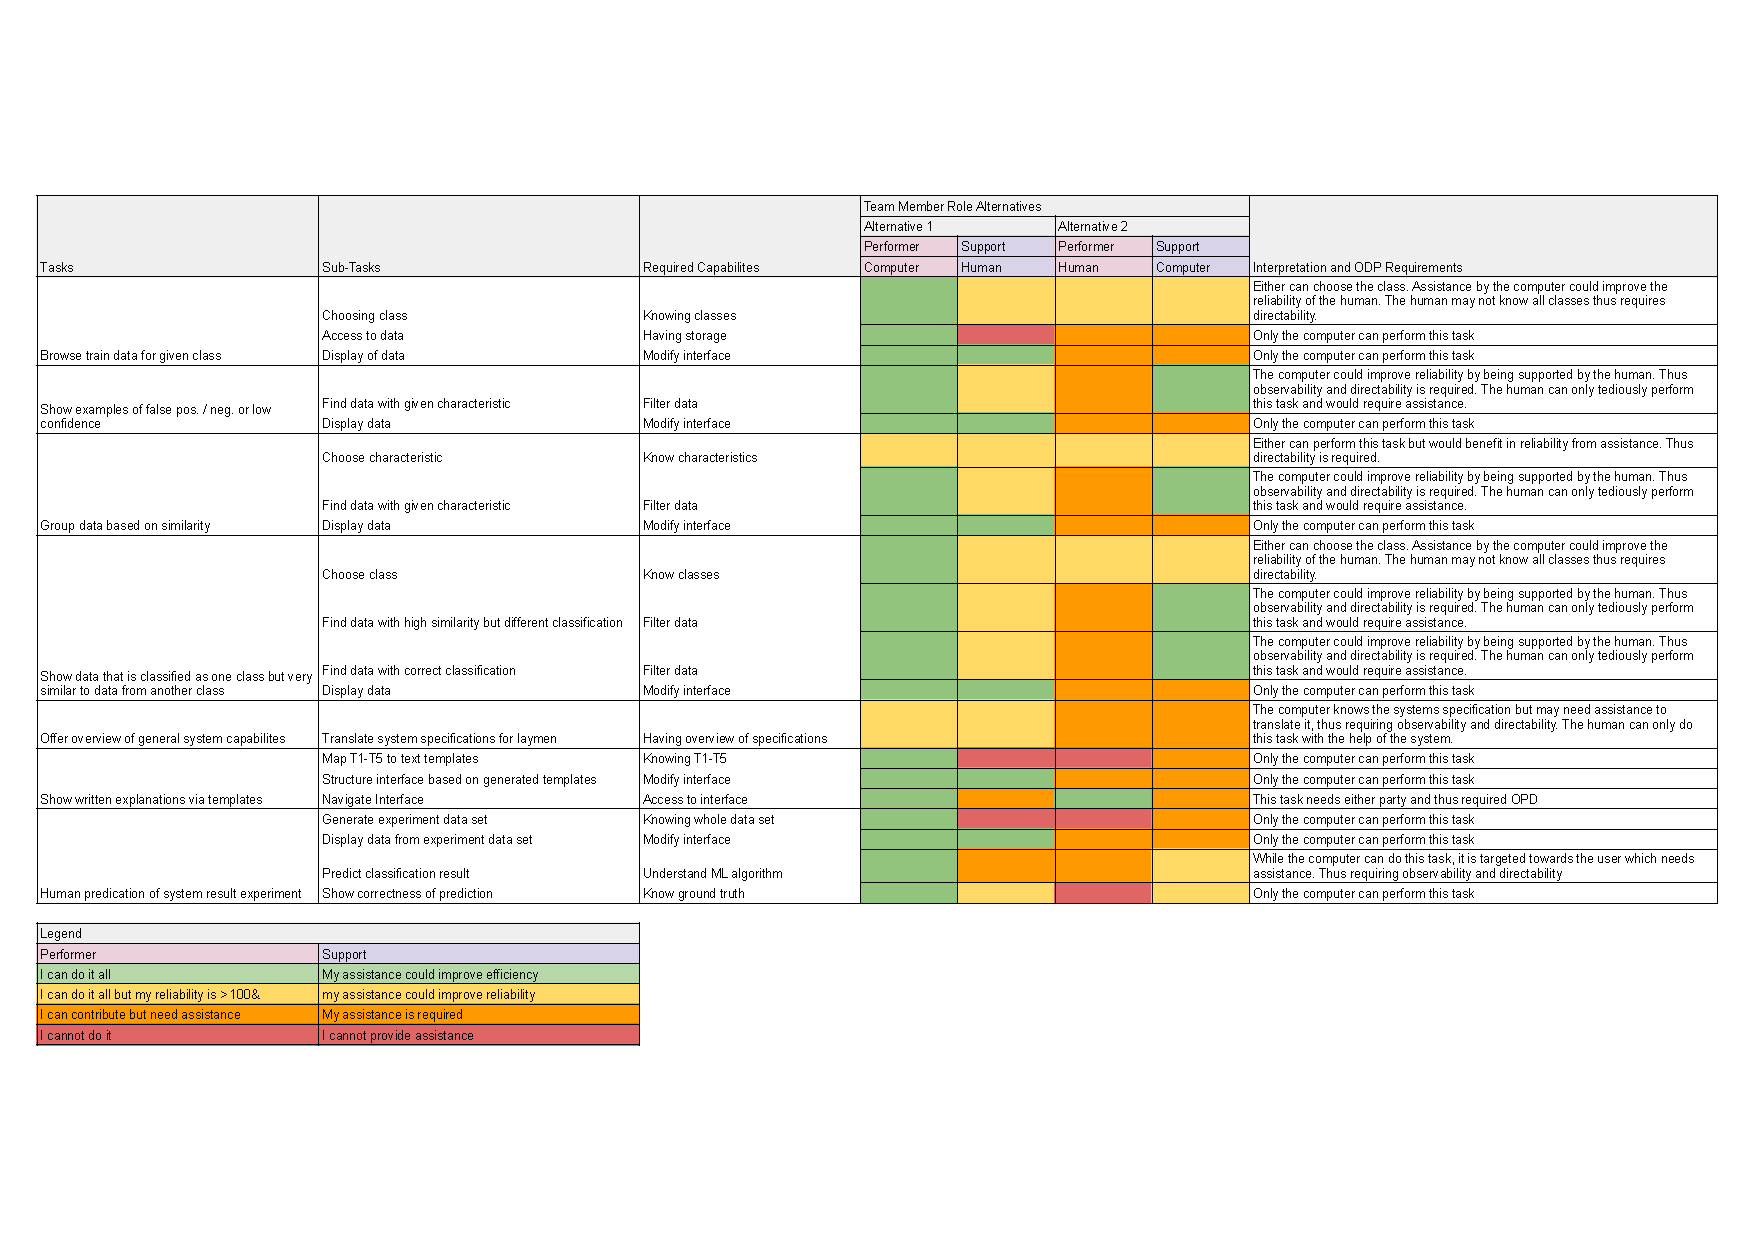
\includegraphics[height=\textwidth, angle=90]{img/figures/Interdependency_Analysis_Table.pdf}
    \caption{Interdependency Analysis Table}
    \label{table:interdependency_analysis_table}
\end{table}

\subsection{Explanation Techniques}\label{subsection:explanation_techniques}
Three groups of explanation techniques are created as possible ways to implement the required functionalities (\autoref{table:function_specification}). The groups are divided by their style of interaction and information deliverance. Most of the presented techniques have a direct mapping to the functionalities to be provided by the assessment system, especially \textit{General Description, Metrics, Data Browsing and Experiment}. The visual explanation techniques though, do overlap significantly in their practicality. While they differ drastically in their mode of operation and technical background, they do cater to the same interaction: Showing image regions that are significant to the result of the AI. Because of this and the limited time and resource frame, only one of the three proposed visual explanation types will be implemented.
\subsubsection*{Textual}
\begin{description}[font=\normalfont\itshape]
    \item[General Description:] General descriptions of the system capabilities aim to explain the system on a level, that is accessible to machine learning laymen, such as medical professionals. As described by \textcite{people_ai_google_website} it is beneficial for building trust when the system capabilities are explained instead of the technology itself. This helps the user to build a better mental model \parencite[p.3]{hoffman_metrics_2019}, especially when dealing with hyper-complex structures, such as DNNs. The general descriptions shall contain a textual explanations of the model capabilities to ensure a good introduction and appropriate expectations.
    \item[Metrics:] Standard metrics are also used to describe the machine learning model. The metrics used are \textit{Accuracy, Precision, Recall \& F1}. Those metrics were chosen, because they are often used to describe ML applications and in the medical context and should therefore be interpretable by medical professionals or data scientists \parencite{sokolova_beyond_2006,hicks_evaluation_2021}. 
\end{description}

\subsubsection*{Interactive}
\begin{description}[font=\normalfont\itshape]
    \item[Data Browsing:] The ability to browse the training data of a machine learning model was universally requested by the interviewed professionals. The browsing ability is extended by different filters for the specific functionality. The user shall be able to explore the training data based on the class of the image. Furthermore the data will be algorithmically grouped based on similarities to potentially expose patterns. Additionally the user shall be able to explore data points that belong to the edge cases of the models capabilities, such as false negative and false positives.
    \item[Experiment:] Comparing the machine learning models predictions to the human expertise also was a key aspect of AI interaction in the medical domain as shown by the interviews. Therefore a input-output-experiment shall be implemented, where the user is able to test the AI against its own expertise.
\end{description}

\subsubsection*{Visual}
\begin{description}[font=\normalfont\itshape]
    \item[Occlusion Sensitivity:] A perturbation based approach to compute attribution, involving replacing each contiguous rectangular region with a given baseline, and computing the difference in output. Occlusion Sensitivity is most useful in cases such as images, where pixels in a contiguous rectangular region are likely to be highly correlated \parencite{captum_website,zeiler_visualizing_2013}.
    \item[Anchors:] The algorithm provides model-agnostic and human interpretable explanations suitable for classification models applied to images, text and tabular data. The idea behind anchors is to explain the behaviour of complex models with high-precision rules called anchors. These anchors are locally sufficient conditions to ensure a certain prediction with a high degree of confidence \parencite{ribeiro_anchors_2018}.
    \item[LRP:] The Layerwise Relevance Propagation (LRP) algorithm explains a classifier's prediction specific to a given data point by attributing (positive \& negative) relevance scores to important components of the input by using the topology of the learned model itself \parencite{lapuschkin_unmasking_2019}.
\end{description}
Referencing the \autoref{chapter:analysis}, the main goal of a visual explanation shall be the validation of the AI model's behavior. Therefore a simple technique, such as Occlusion, which only highlights image regions with a high importance to a result, is reasonable and easy to implement for any DNN. While LRP does have certain benefits because of its ability to assess positive and negative influences of pixels to the model output, it also comes with a high complexity that manifests as a lot of hyperparameters, making it hard to implement and use properly. Anchors work differently to the other two methods, since it is able to find a hyperpixel that is most influential to a AI's classification and thereby highlight image areas that are sufficient for the classifier's decision. Although all visual methods seem fitting for the explanation task, only Occlusion Sensitivity shall be implemented as to provide a simple to interpret visual explanation technique with a manageable implementation complexity. Additionally implementing and showing the user multiple visual explanation techniques could lead to contradicting explanations and a negative impact on the user in this context.

\section{System Architecture}\label{section:system_architecture}
The goal is to create an interactive software application, therefore a suitable system architecture has to be constructed to suite the needs of the users and the usage context. Although, implementing the functionalities from \autoref{section:functionalities} is possible in many different ways. It is possible to realize the assessment system as a classical, offline software application or by leveraging web based tool sets for a possibly distributed cloud solution. Also it is conceivable to implement the system on a middle ground of those two, by creating a software that is build to be ran locally in common web browsers. These three options will be shortly evaluated against each other based on the requirements set by the functionalities while staying hardware and software agnostic. 

The common requirements are the ability to store machine learning models and training data for the assessment to be computed. In addition the user has to be presented with a graphical user interface (\textbf{GUI}) to interact with. Having these two components in a close relation can drastically reduce the overhead of implementing the communication between the computational and data storage component with the GUI component. On the other hand such a close relation in an offline system can significantly reduce the flexibility of the implementation regarding GUI and interaction design. Furthermore a single offline application has to take many different execution environments (operating systems) into account, which might be a big downside depending on the actual context of usage. Separating the system into a multi-tier application allows for more modularity and freedom in choosing the actual implementation technology. A multi-tier web application allows for a very specialized choice of tools for the respective component at the cost of a higher complexity and implementation cost. Such web applications have the advantage of being relatively easy to transform into a local application without the need of hosting a server environment. This can be the middle ground between the offline local and the web based distributed application.

Referencing the usage context of the application it is not needed to implement a highly complex distributed application, although Clearbox has shown that it is very much possible to implement a robust cloud based solution. To reduce the scope of implementation for this thesis a middle ground is the most reasonable: Leveraging modern web based tools that are mostly environment agnostic to build a flexible application that could be ran in either the cloud or locally on a single machine. \autoref{fig:system_architecture} shows a possible system architecture for a two-tiered application, where the GUI is separated from the logic and the data store. Such a separation of concerns on the macro level enables the usage of specialized tools for each component. While it is conceivable to move the data store into a separate tier (making it a three-tiered architecture), there are no concrete requirements for using a individual data store technology, such as a dedicated database.

The \textit{frontend} component encompasses the user interface, which will probably be realized with web-based tools as mentioned before. This web-based component facilitates the flexibility of the implementation, as the user will remain mostly hardware and software independent by leveraging common browser technologies. The \textit{backend} will be decoupled from the GUI and therefore can benefit from other technological stacks, optimized for the tasks of machine learning and data science. Additionally the backend will envelop the data and the AI model itself, for providing its services to the frontend. This split allows for a distributed, hardware and software agnostic architecture which can be run either locally or remotely, whereas leveraging the optimal tools for each task.

The communication between the two components will be realized through an \textbf{API}. The protocol used for such a communication will be the standardized \textit{Hypertext Transfer Protocol}, which allows for systems
to be built independently of the data being transferred \parencite{rfc2616}.

\begin{figure}[htbp]
    \centering
    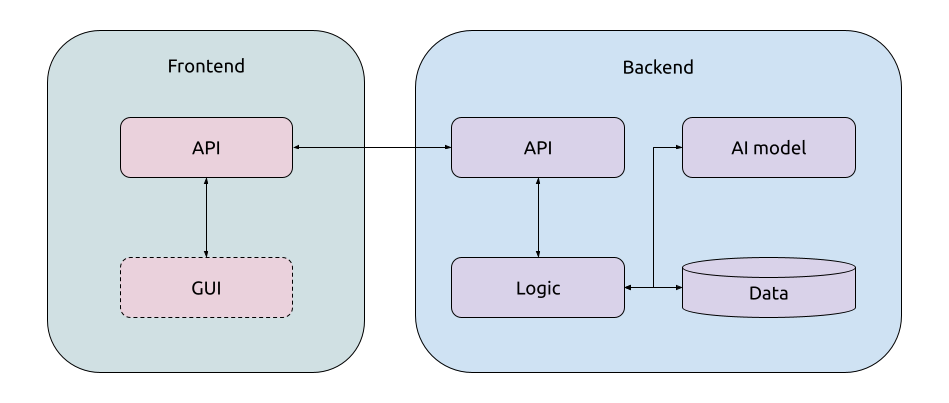
\includegraphics[width=\textwidth]{img/figures/architecture.png}
    \caption{Multi Tier System Architecture}
    \label{fig:system_architecture}
\end{figure}

\section{Interaction Design}\label{section:interaction_design}
The interaction design is a key aspect of HCI, as it defines how the user will actually interact with the system and how information will be made accessible to the user. Considering the human factors in the design process is very important as described by \textcite{wickens_2016_engineering} - for this builds upon the insights of the previous chapters, namely the definition of interaction (sub-)tasks and the interdependency analysis, which in turn are based on the general objectives and user needs as described in \autoref{chapter:analysis}.

The conception of functionalities and interaction design was the main topic of the previously mentioned expert workshop, which was conducted with colleagues from the university of Lübeck and Clearbox. The goal was to present, validate and discuss the scope of functionalities and the interaction design which utilizes scaffolding and guidance for the main user group. Guidance in HCI, as described by \textcite{trigg_guided_1988}, aims to help the user with navigating and effectively utilizing a software artifact by providing predefined paths through the contents of an application, possibly based on the user's interests or intentions. The workshop yielded good feedback on the scope of functionalities and the guidance concept. The focus of the discussion was the type of guidance which was then resolved to a semantic signal manifested by an intention query that defines which functionalities are displayed. Other relevant results of the workshop were: (1) The identification of a possible contradiction between different visual explanation techniques, which were described in \autoref{subsection:explanation_techniques}. This reinforces the idea to limit the visual explanations to one to avoid unnecessary confusion of the user. (2) Feedback from Clearbox's own tests showed the tendency towards a more sequentially user experience in contrast to a dashboard centered application. (3) Pre-computation of computationally expensive explanation methods to eliminate performance bottlenecks and increase the response time of the application.

A central consideration of the interaction design is to adapt the system to the abilities and needs of the actual users. Referencing \autoref{subsection:interviews}, a main user group has low expertise in machine learning, which in turn means special requirements for the interaction design of an AI assessment system. Therefore the design approach will revolve around a guided interaction version and a unguided interaction version: The guided interaction will leverage a more streamlined approach which facilitates the intentions of the user by asking and then presenting the respective functionality. \textcite{trigg_guided_1988} already proposes local guidance of the user by the author of a system, by using intention queries to determine a suitable path through the content of an application. This mode of interaction aims to relieve the user of mental workload by scaffolding the application and thus avoiding the presentation of all functionalities, and therefore aiding the learning process for machine learning topics \parencite{soloway_learner_1994}. The other mode of interaction will be unguided, as in there will be no intention query and the user will be able to freely explore the whole lot of functionalities offered by the application, which is hypothesize to be beneficial for users with more expertise in machine learning. The baseline for both ways of interaction is the whole array of functionalities as specified in \autoref{table:function_specification}.

To further explore and concretize the interaction design two methods were applied: \textit{Interaction Dialogues} and \textit{Interaction Flowcharts}. Interaction dialogues aim to creatively explore different ways of implementing the functionalities as defined in \autoref{section:functionalities}. Additionally they enable the exploration of other perspectives based on a natural interaction mode (spoken dialogue). The result is then the baseline for the interaction flowcharts, which specify the concrete flow of information in a standardized manner.

\subsection{Interaction Dialogues}\label{subsection:interaction_dialogues}
Using dialogues as the mode of interaction and communication between human and computer leverages a representation of the user and use context as a fixed set of well defined goals, tasks or needs \parencite[p.4]{wright_user_2005}. \todo{check citation} The goal was to explore different variations of interaction based on the functionalities as defined in \autoref{table:function_specification}. An example dialogue (with H for human and C for computer) for task 1 will be presented:
\begin{displayquote}
    H: I would like to see your training data.\\
    C: Do you want to see all data or just data for a specific class?\\
    H: I want to only see data for class X.\\
    C: Here you go! Do you want to see data of another class, too?\\
    H: Yes please, but give me some time.\\
    C: Of course!
\end{displayquote}

Using the dialogue technique allows for easy exploration of alternative information flows as shown by the next example:
\begin{displayquote}
    H: I would like to see your training data.\\
    C: Here take a look!\\
    H: Wow, that is really a lot!\\
    C: Do you want to filter for a specific class?\\
    H: Yes, please show me only data for class X.\\
    C: There you go.\\
    H: Thank you, and now please show me all data for class Y.\\
    C: Sure, here!
\end{displayquote}

These examples clearly show different ways of interacting in order to accomplish the same task (browsing the training data). This process was applied to all tasks from \autoref{table:interdependency_analysis_table} to gather a lot of different interaction variations, to be then used as a baseline for the following interaction flowcharts. The key takeaways from this process, was that there are various possibilities to realize an interaction. With multiple alternatives per task, some comparisons could be made: Often it seems beneficial for a streamlined interaction design, to present the user with a set of options from the beginning, instead of presenting everything and then reducing the amount of information. Furthermore situations with exhaustive searches can be avoided by presenting the user a limited amount of information. Most tasks had two to three alternatives which were compared against each other in order to find the best dialogue, which was then chosen to be the baseline for the standardized flowcharts.

\subsection{Interaction Flowcharts}\label{subsection:interaction_flowcharts}
Flowcharts were used to formalize the functionalities (see \autoref{section:functionalities}) with the insights of \autoref{subsection:interaction_dialogues}. The type of flowchart is defined in \textit{DIN 66001} \parencite{hering_programmablaufplan_1984}. The flowcharts are essential as a reference for the implementation, as they define the details of the information flow between the two parties. The goal is to have interactions that have a clear start and end point, with no dead ends, while also identifying loops. Flowcharts allow for the validation of these goals. Another goal was to separate the application into small, manageable interactions, each defined by its own flowchart. \autoref{fig:flowchart_browse_data} shows a flowchart that defines the flow of interaction for the process of browsing classified images (task 1 from \autoref{table:function_specification}), with the background of the presented interaction dialogue. For each of the tasks defined in \autoref{table:function_specification} and \autoref{table:interdependency_analysis_table} such a flowchart was developed as seen in \nameref{appendix:interaction_flowcharts}.
\begin{figure}[htbp]
    \centering
    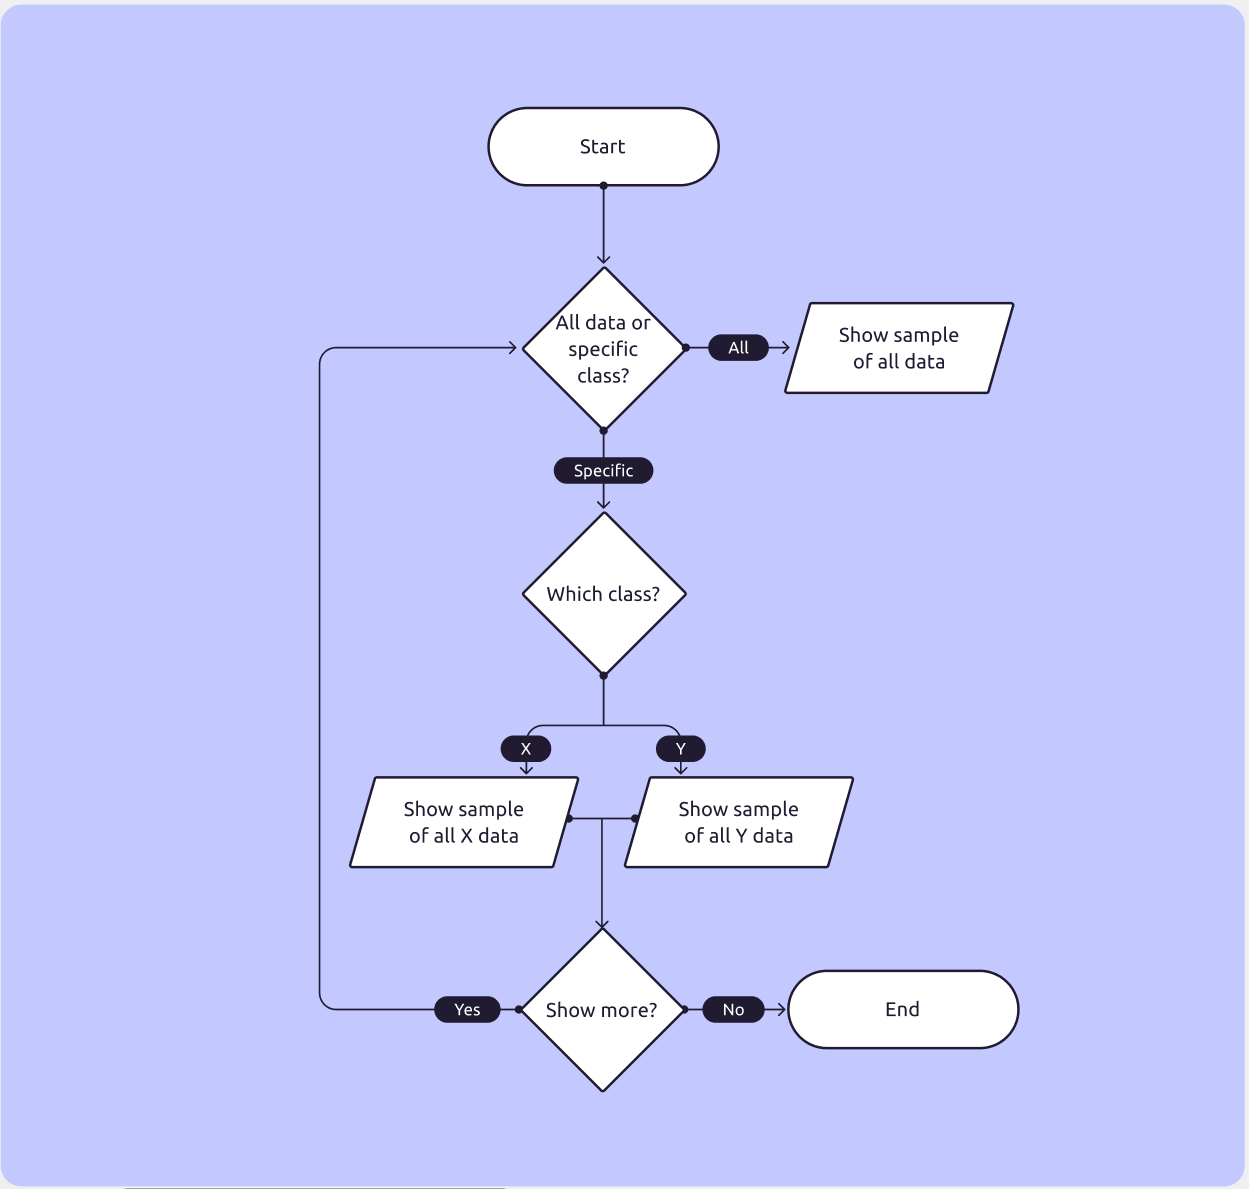
\includegraphics[width=\textwidth]{img/figures/flowcharts/browse_train_data_for_chosen_class.png}
    \caption{Flowchart - Browse Training Data for a given Class}
    \label{fig:flowchart_browse_data}
\end{figure}

\section{Interface Design}\label{section:interface_design}
Based on the functional specification and the interaction design an interface design was developed to encompass the whole array of functionality into a single application. Similar to the flowcharts, the application interface can be differentiated into single elements of interaction as defined by the tasks and interaction flowcharts. This separation allows for a better overview and a more flexible layout. Additionally inspiration was drawn from the state-of-the-art application from Clearbox as seen in \autoref{section:state_of_the_art}, where a similar approach was chosen. The concept of splitting the application into smaller pieces also facilitates the usability of the whole application, as the user will not be overburdened with all functionalities simultaneously \parencite[p.159]{demerouti_psychische_2012}. Instead the user will be able to choose which functionality he wants to utilize. Additionally, the functional elements shall be included in boarders to visually group GUI elements that belong together \parencite{kohler_gestalt_1967}. This layout goes hand in hand with the guidance concept, as every functionality will be represented as its own part of the user interface. This is an important aspect to consider, especially regarding the reusability of software components. Furthermore, preventing multiple implementations of the same functionality helps with the comparability of the guided versus non-guided version of the application.

The interface design is optimized for devices with relatively big screen sizes, such as desktop computers, laptops or tablets as there was no use case found for a smartphone application (see \autoref{chapter:analysis}). Additionally the screen size is needed for the user to properly view the image content. As such the layout of the application will be vertically scrollable, supporting landscape and portrait orientations to match the devices and the use case.

\autoref{fig:mockup_part_1}, \autoref{fig:mockup_part_2} and \autoref{fig:mockup_part_3} show a mockup of the application, designed as a single page layout with all functionalities present. The layout presented here corresponds to the unguided version. On the top of the application (\autoref{fig:mockup_part_1}) general information about the model, its capabilities and standard metrics are shown. Further down (\autoref{fig:mockup_part_2}) the data browsing functionalities are depicted. Lastly the the similarities and the experiment functionalities are shown at the bottom of the application (\autoref{fig:mockup_part_3}). Furthermore the order of the components is determined by the level of involvement needed of the user: The beginning is limited to higher level information, which then transforms into a deeper insight into the training data, model limitations and clustering of data, and concludes in the input-output experiment where the user can test its mental model against the actual AI.

The general design of the application revolves around a simple modern layered design in the form of cards with rounded corners. This aims to make the single components easily distinguishable while preventing the introduction of unnecessary visual separations. The color theme of the application is chosen to be neutral with high contrast between text and background while utilizing highlighting colors for important interface components for good readability and easy orientation. Although this mockup heavily references Clearbox' design language, a additional dark mode with inverted colors is considered depending on the user preferences and image content.

\begin{figure}[htbp]
    \centering
    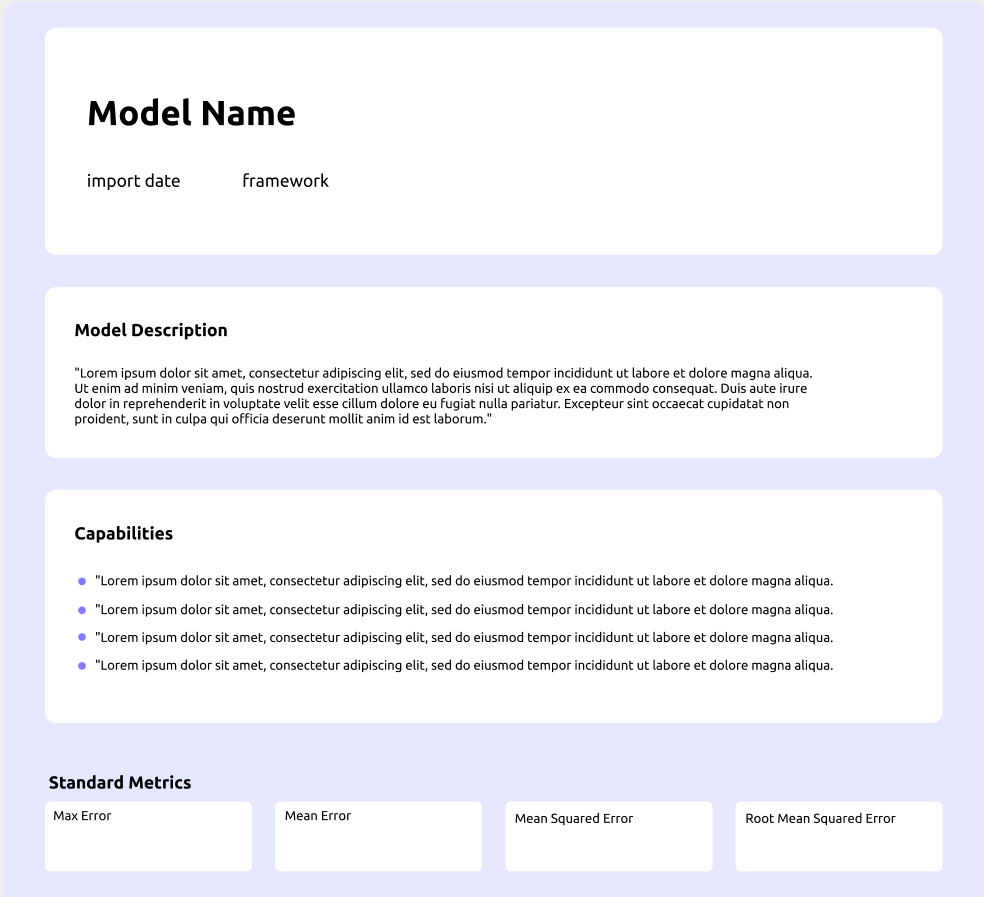
\includegraphics[width=\textwidth]{img/figures/mockups/mockup_1.png}
    \caption{Mockup Part 1}
    \label{fig:mockup_part_1}
\end{figure}

\begin{figure}[htbp]
    \centering
    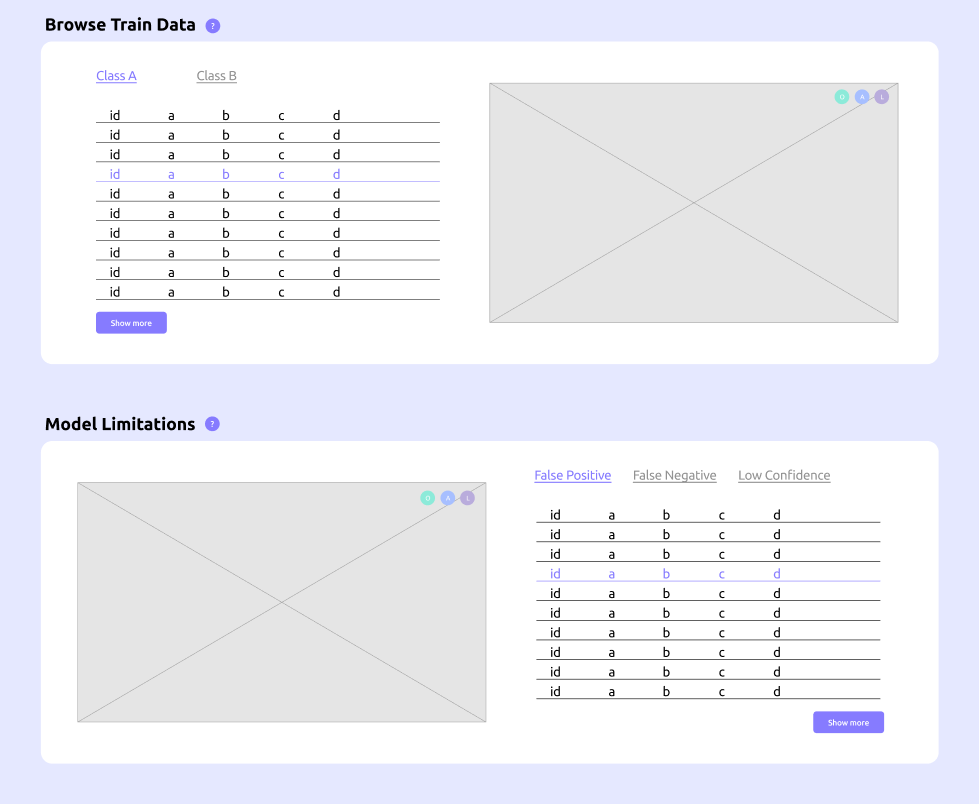
\includegraphics[width=\textwidth]{img/figures/mockups/mockup_2.png}
    \caption{Mockup Part 2}
    \label{fig:mockup_part_2}
\end{figure}

\begin{figure}[htbp]
    \centering
    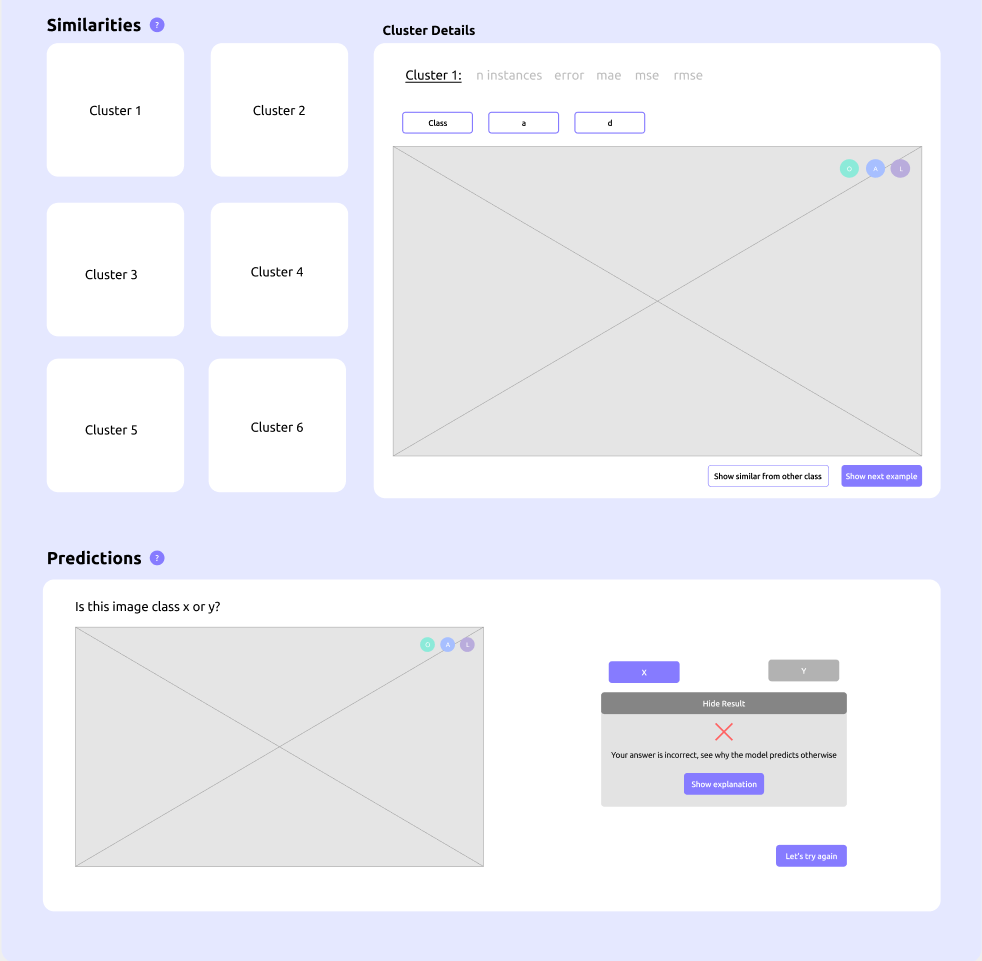
\includegraphics[width=\textwidth]{img/figures/mockups/mockup_3.png}
    \caption{Mockup Part 3}
    \label{fig:mockup_part_3}
\end{figure}

\section{Conclusion on the Conception}
Through the use of functional specifications, interaction and interface designs, possible solutions were conceptualized to meet the requirements of the user, the usage context and the overall goals. By referencing the concrete use cases and user requirements seven functionalities were derived (see \autoref{table:function_specification}), which were then analysed for interdependencies in a HCI scenario, resulting in a specification of tasks, sub tasks and capabilities required to perform those for either party of the interaction (see \autoref{table:interdependency_analysis_table}). The used explanation methods are described in detail in \autoref{subsection:explanation_techniques} and insights were collected about the mapping of the functionalities to the explanation techniques, while providing a semantic grouping for those techniques. Although many explanations techniques have a direct mapping, the visual explanation was overrepresented and Occlusion Sensitivity was chosen to be the only visual method to be implemented to avoid multiple possibly contradicting visual explanations. Complementing the functional specification, a technical system architecture (see \autoref{fig:system_architecture}) was conceptualized, which is constructed with flexibility in mind, leveraging modern web based technologies while meeting the requirements of an AI assessment system. A conceptional iteration via an expert workshop helped validating and improving concepts, such as guidance, and the functional scope. Interaction dialogues (see \autoref{subsection:interaction_dialogues}) for the seven tasks allowed for the exploration of interaction variations per task. Furthermore interaction flowcharts (see \autoref{subsection:interaction_flowcharts}) were defined to specify the concrete flow of information between the interacting parties and as the main reference for the implementation logic. The functional components manifested in an interface design mockup (see \autoref{section:interface_design}), which leverages the interaction design and the idea of guided versus non guided interaction styles to provide a GUI for users with various expertise in machine learning. The interaction and interface concept aims to provide two separate GUIs that build on the same flexible components, each encompassing one functionality, to be later evaluated against each other.

\newpage
\chapter{Implementation}\label{chapter:implementation}
The AI assessment system will be implemented based on the insights and conclusions from \autoref{chapter:conception}. The system to be build has to realise many tasks from the data science and machine learning domains while it also needs to provide a GUI for user interaction, as described by \autoref{section:system_architecture}: Implementing the AI assessment system prototype as a flexible, hardware agnostic application is a main goal of the system architecture and implementation, while also meeting the interaction and design requirements as described in \autoref{section:interaction_design} and \autoref{section:interface_design}.

Taking these aspects into account, a \textit{Python} based backend implementation is preferable, as the programming language is widely used for data science and machine learning tasks, while also providing tools for web application building. Furthermore Python ranks the most popular programming language as of november 2021 and provides some of the most used and curated software libraries for data science and machine learning among all alternatives \parencite{toibe_index_python_website,numpy_github,pandas_github,pytorch_website}. The flexibility provided by Python allows the backend to be completely implemented in said language and making no compromises on the tools needed.

Being decoupled from the machine learning domain, the possible frontend implementation tool set is much more diverse: Popular frameworks for browser based GUIs are \textit{React}, \textit{Angular} and \textit{Vue} (amongst others), all providing the required functionalities in either \textit{JavaScript} or \textit{TypeScript} in combination with the classic \textit{HTML} and \textit{CSS} technologies.

Referencing \autoref{subsection:existing_apps} and Clearbox, a Python based application leveraging \textit{Streamlit} will be used for implementing the AI assessment system \parencite{streamlit_website}. While there are many different possible alternatives to implement such a flexible distributed system (for example \textit{Django} or \textit{Flask} in combination with \textit{React}), Streamlit comes with a big advantage: The ability to directly transform Python scripts into deployment ready web applications including a GUI. This ability completely invalidates the disadvantage of building a flexible web based application, as it avoids the additional effort of implementing the communication between the presentational and the logic layer of a multi-tier application. Although strictly speaking a Streamlit-based application will not be multi-tiered in its implementation as it only consists of singular python scripts leveraging the Streamlit platform, which in turn hides most of the complexity of implementing a distributed, web based application. Additionally some flexibility in implementing the actual frontend of the application is lost by using such a omnipotent library, as there is no need for a specialized GUI technology. However it is reasonable to limit the implementation complexity of an AI assessment system prototype in the scope of this thesis by leveraging the Streamlit framework.

Also in this conjuncture, it makes sense to limit the implementation complexity of a AI model to be used in the assessment system. Instead of developing a own model, a pre-trained model was chosen. The model used for the implementation of the assessment system prototype is the \texttt{densenet121-res224-rsna} model from \textcite{cohen_torchxrayvision_2021}. The model is part of an open source software library called \textit{TorchXRayVision} for working with chest X-ray data sets and deep learning models. It provides a common interface and common pre-processing chain for a wide set of publicly available chest X-ray data sets. This concrete model was trained to classify X-ray images and therefore detect a pneumonia disease. Additionally the fitting and also publicly available \textit{RSNA Pneumonia Detection Challenge} data set was used \parencite{rsna_kaggle_website}. Leveraging a pre-trained model and a curated data set is an important aspect in the implementation of an AI assessment system, as it perfectly resembles an application scenario for the medical domain and therefore supports the implementation of the actual assessment system in the context of this thesis. However, for a complete assessment system implementation, a functionality for importing any machine learning model and data set would be needed - this was omitted, as it is not essential for the evaluation of AI explanation method effects on users.

The whole source code of the AI assessment system prototype can be found digitally on DVD in \nameref{appendix:dvd_contents} or online on Gitlab\todo{make repo available}. The following sections will reference parts of the source code when needed.

\section{System Architecture Implementation}
Using the Streamlit platform implies some changes to the originally conceived system architecture (see \autoref{fig:system_architecture}). The Streamlit platform allows building a whole web-based application with just Python code, and therefore eliminates the need to implement a separate frontend and the communication between the frontend and the backend. Based on the platform's focus on data science tasks, all functionalities (\autoref{table:function_specification}) can be implemented with the provided GUI elements. \autoref{fig:architecture_implementation} showcases the adapted system architecture, which leverages the Streamlit platform: The frontend shrunk to a thin client, which runs in the browser. The frontend consequently only consumes the service provided by the backend and is responsible for displaying the GUI elements to the user. Furthermore the actual implementation of the GUI elements is already provided by Streamlit: Based on the Python scripts in the backend, GUI elements are generated by Streamlit for the browser to display (see \autoref{section:interface_implementation} for details). The backend is now embedded in the Streamlit platform and makes use of its API to generate a multi-tier web application by using the provided tools. The internal structure of the backend has not changed and still includes a logic component, the AI model and a data store. The communication between the frontend and the backend is realized via the HTTP protocol as described in \autoref{section:system_architecture}.

\begin{figure}[htbp]
    \centering
    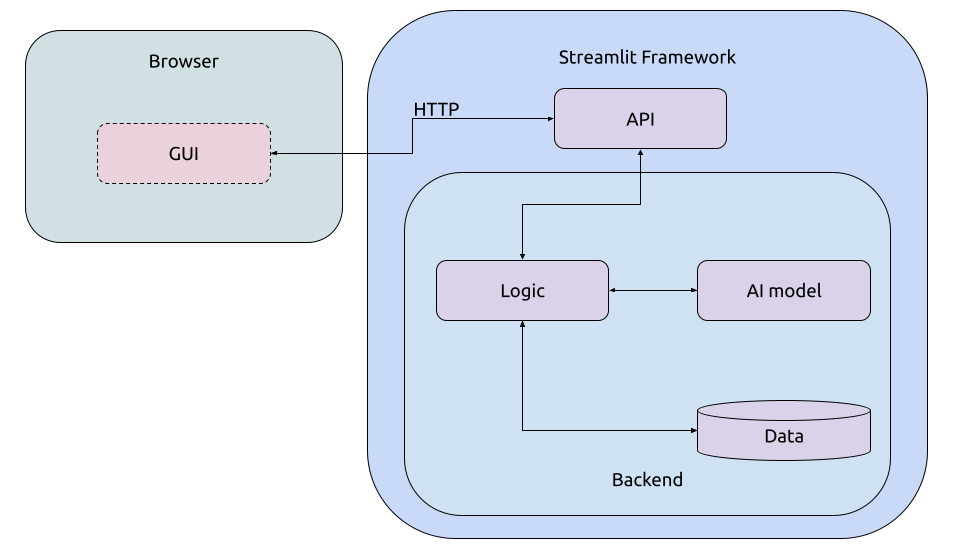
\includegraphics[width=\textwidth]{img/figures/architecture_implementation.png}
    \caption{System Architecture Implementation with Streamlit}
    \label{fig:architecture_implementation}
\end{figure}

The implementation was split up into two modules, the logic component which handles the user interaction and uses the Streamlit API and the data component which outsources some common functionality regarding data acquisition, transformation and provision. For a basic separation of concerns, these modules were split into two files, where the logic component makes use of the data component, which in turn makes use of the \textit{scikit-learn} and \textit{TorchXRayVision} libraries. Because of the heavy usage of the Streamlit platform, the total system architecture implementation is simple in comparison to a complete multi-tiered solution built on separate technological stacks.

\autoref{listing:main.py_initialization} and \autoref{listing:data_module_usage} show the utilization of the \textit{TorchXRayVision} library and the interaction of the logic module with the data module to load the AI model and RSNA data set for the assessment system to use. Take note of the \python{@st.cache} annotation, which makes use of the Streamlit API to identify data that can be cached for improved performance. This is especially useful for CSV data, that is readily displayed in the GUI. \autoref{listing:main.py_initialization} and \autoref{listing:data_module_usage} are the foundation for the backend component, which builds on top of the AI model, loaded data and Streamlit API. \autoref{table:software_versions} shows the primary software used for the implementation of the whole system.

\begin{listing}[htpb]
    \begin{minted}{python}
        model_specifier = 'densenet121-res224-rsna'
        model = xrv.models.DenseNet(weights=model_specifier)
        d_rsna = load_rsna_dataset()
        detailed_class_info = load_detailed_rsna_class_info()
        classes = detailed_class_info['class'].unique()
    \end{minted}
    \caption{Initialization of the Model and Data Set}
    \label{listing:main.py_initialization}
\end{listing}

\begin{listing}[htpb]
    \begin{minted}{python}
        @st.cache
        def load_rsna_dataset():
            d_rsna = xrv.datasets.RSNA_Pneumonia_Dataset(
                imgpath='./data/kaggle-pneumonia-jpg/stage_2_train_images_jpg',
                views=["PA", "AP"],
                unique_patients=True,
                transform=transform)
            return d_rsna

        @st.cache
        def load_detailed_rsna_class_info():
            return pd.read_csv('./data/kaggle-pneumonia-jpg/stage_2_detailed_class_info.csv')
    \end{minted}
    \caption{Functions for Image and Meta Data Acquisition}
    \label{listing:data_module_usage}
\end{listing}

\begin{table}[htbp]
    \centering
    \begin{tabularx}{0.3\textwidth}{ l l }
        \toprule
        software & version \\
        \midrule
        Python & 3.9.6 \\
        captum & 0.4.1 \\
        numpy & 1.21.2 \\
        pandas & 1.3.3 \\
        scikit-learn & 1.0.1 \\
        streamlit & 1.2.0 \\
        torch & 1.9.1 \\
        torchxrayvision & 0.0.32 \\
        \bottomrule
    \end{tabularx}
    \caption{Used Software and Versions}
    \label{table:software_versions}
\end{table}

\section{Interface Implementation}\label{section:interface_implementation}
Based on the concepts of \autoref{section:interaction_design} and \autoref{section:interface_design} the interface was implemented using the tools and GUI elements of the Streamlit platform \parencite{streamlit_github}. The mainly used GUI elements were: \texttt{expanders}, \texttt{columns}, \texttt{tables}, \texttt{images}, \texttt{buttons}, \texttt{checkboxes} and \texttt{selectboxes} - all of which are readily provided. To aid the visual impression of the system, specifically for the display of Xray images, a dark interface mode was made the default, while the user still had the option to change to a bright mode.

As conceived in the conception, all functionalities were implemented as differentiated GUI components by using the \texttt{expander} element. \autoref{listing:overview_element} showcases the implementation of such an component, which makes use of the \texttt{expander} element in combination with the \texttt{columns} horizontal layout functionality. Specifying the GUI elements with Streamlit builds upon a very structured and sequential convention: Items are presented in the same order, as they are declared in the Python code (with the exception of column layouts). There are very few possibilities to specify complex layout concepts, which automatically results in a very clean and structured GUI. \autoref{fig:overview_element} shows the rendered GUI element which was specified in \autoref{listing:overview_element}. The special feature of an \texttt{expander} element allows for easy hiding or showing of the encapsulated functionality. \autoref{fig:descriptive_elements} and \autoref{listing:descriptive_elements} show this exact feature: Multiple functionalities are declared successively with the \texttt{expander} element, but only one item is chosen to be presented by the user by clicking on it.

Managing the state of the application is an important aspect, as it allows for the individualization of the user experience. This is particularly relevant for the implementation of the intention query as conceived in \autoref{section:interaction_design}. The GUI components provided by Streamlit are inherently stateful, data-driven and have a simple life cycle that refreshes on every interaction, which leads to a simple development process that is backed by the underlying data. However it is more complicated to manage state, that is not tied to specific elements and therefore exceeds the life cycle of the element. An example for this is the random choice of image samples to be displayed to the user: The random data points are sampled for each user of the application and shall only be regenerated if the user whishes to do so (see \autoref{figure:flowchart_browse_data}). Because of the simple life cycle of Streamlit GUI elements, which resets on every interaction, a separate state for some GUI elements has to be managed as seen in \autoref{listing:managing_state}. Streamlit provides a functionality to persist session state per user, which is then saved on the frontend side - this allows a interactive, stateful user experience which is backed by a common data store.

Another important aspect of the interface implementation is the use of the AI model and visual explanation techniques as conceived in \autoref{subsection:explanation_techniques}. To implement the \texttt{densenet121-res224-rsna} model the \textit{torch} library was used. Loading the AI model with this library allows for direct interaction with it, for example the input-output experiment as described in \autoref{section:functionalities}. Furthermore the usage of the \textit{captum} library allowed for the computation of visual explanations (attribution by occlusion) for the data set at hand. To increase the performance of the GUI, the explanations were generated beforehand and saved separately to the original image data including the same unique identifier. \autoref{listing:occlusion} shows the computation of occlusion samples, where each sample results in an image similar to \autoref{fig:occlusion}. The computed images reveal high value super-pixels that indicate a high relevance for the AI model. These samples are then used alongside the original Xray images in the assessment system, where the user can choose to display the context-bound visual explanation.

\begin{listing}[htpb]
    \begin{minted}{python}
        with st.expander('Overview'):
            st.subheader(f'{model_specifier}'.upper())
            overview_l, overview_r = st.columns(2)
            overview_l.text(f'Import Date: {datetime.date.today()}')
            overview_r.text('Framework: Pytorch')
    \end{minted}
    \caption{Overview GUI Element}
    \label{listing:overview_element}
\end{listing}

\begin{listing}[htpb]
    \begin{minted}{python}
        with st.expander('Overview'):
            # [...]

        with st.expander('Model Description'):
            # [...]

        with st.expander('Capabilities'):
            # [...]

        with st.expander('Standard Metrics'):
            st.subheader('Standard Metrics')
            metrics1, metrics2, metrics3, metrics4 = st.columns(4)
            metrics1.metric(label='Accuracy', value=str(metrics['accuracy'].round(2)))
            metrics2.metric(label='Precision', value=str(metrics['precision'].round(2)))
            metrics3.metric(label='Sensitivity', value=str(metrics['recall'].round(2)))
            metrics4.metric(label='F1', value=str(metrics['f1'].round(2)))
    \end{minted}
    \caption{Descriptive GUI Elements}
    \label{listing:descriptive_elements}
\end{listing}

\begin{figure}[htbp]
    \centering
    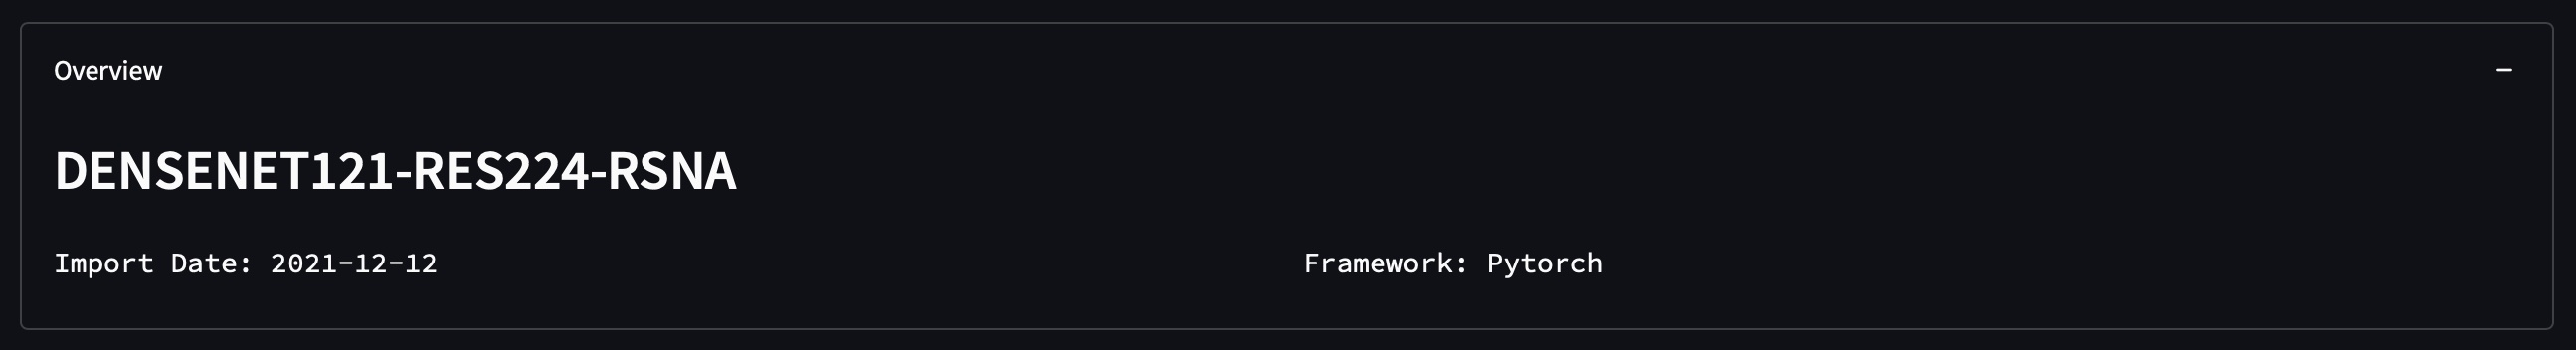
\includegraphics[width=\textwidth]{img/screenshots/overview_element.jpg}
    \caption{Overview GUI Element}
    \label{fig:overview_element}
\end{figure}

\begin{figure}[htbp]
    \centering
    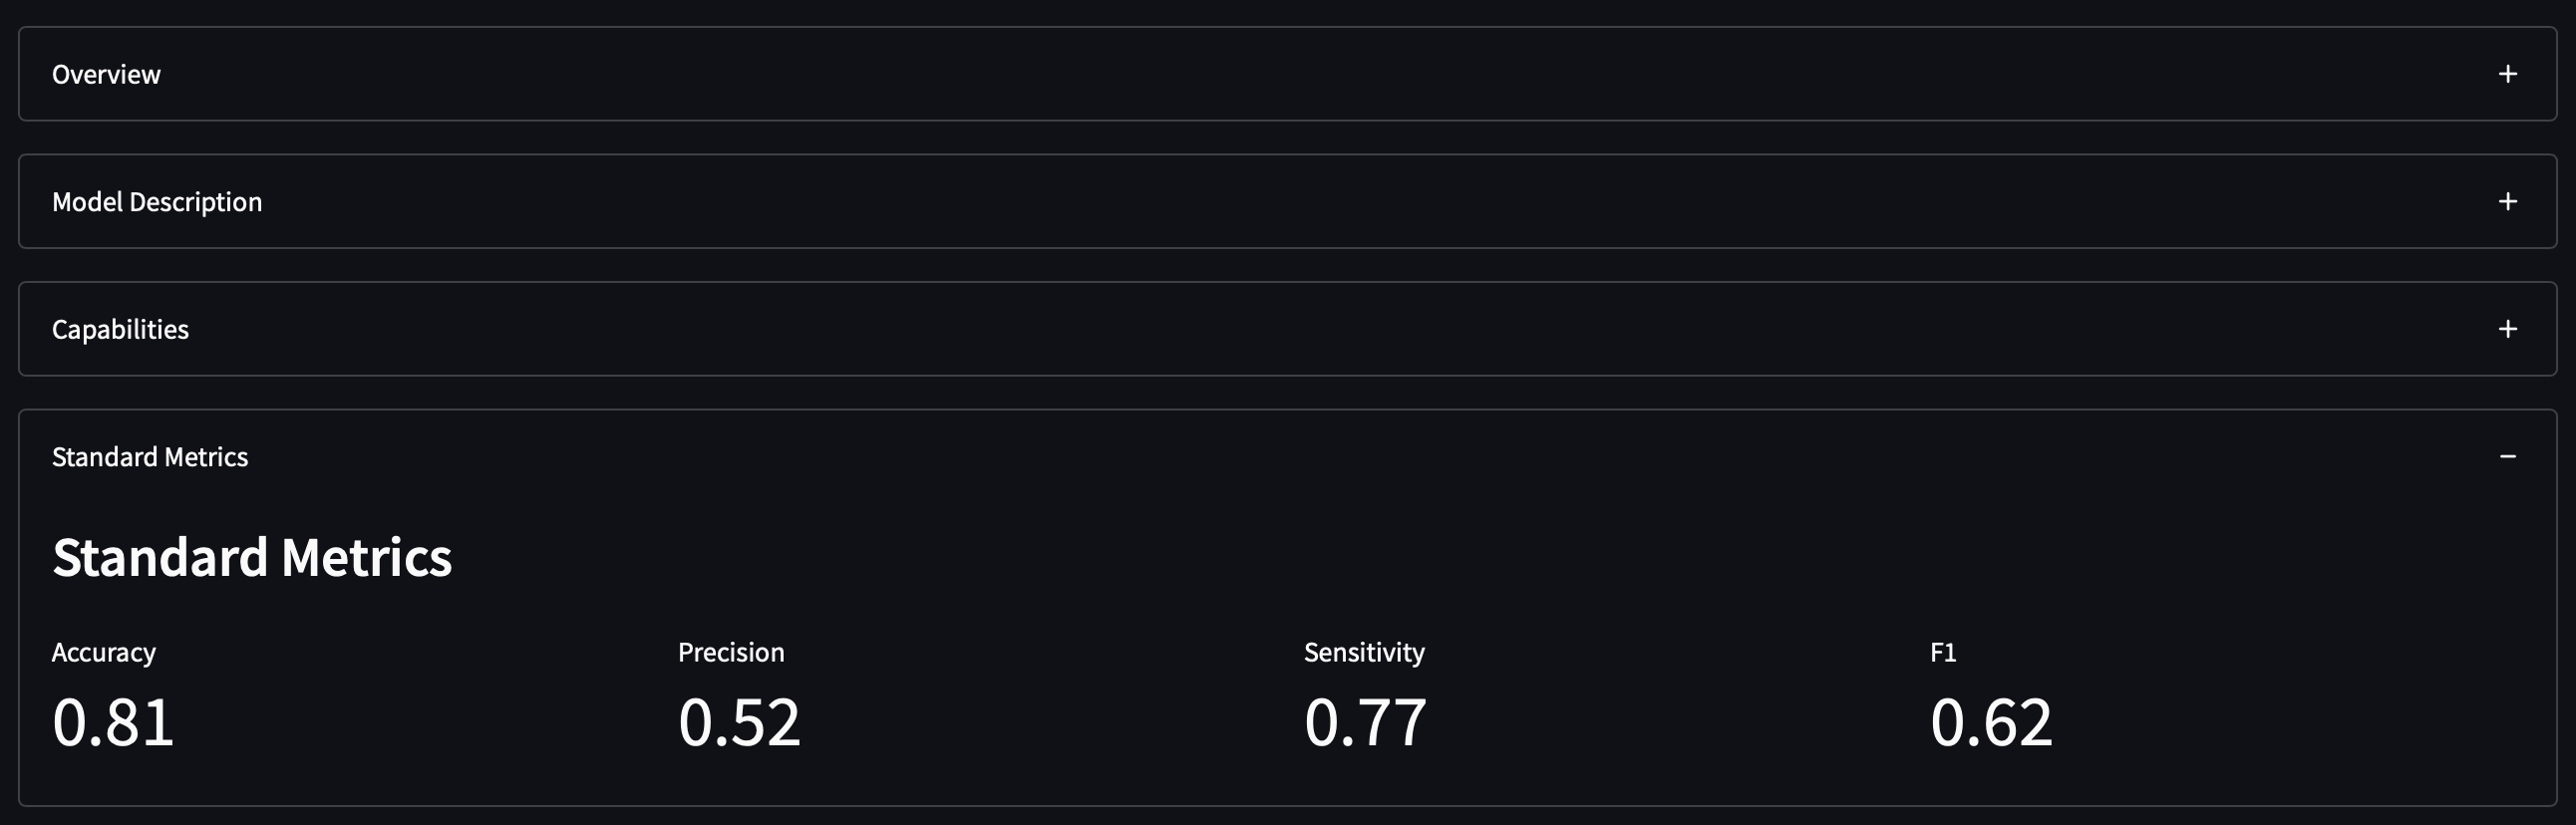
\includegraphics[width=\textwidth]{img/screenshots/descriptive_elements.jpg}
    \caption{Descriptive GUI Elements}
    \label{fig:descriptive_elements}
\end{figure}

\begin{listing}[htpb]
    \begin{minted}{python}
        def set_browse_indices(high):
            st.session_state.indices = np.random.randint(low=0, high=high, size=10)
        # [...]
        if 'indices' not in st.session_state:
            set_browse_indices(len(dataset.index))
        index_list = st.session_state.indices
        df_samples = dataset.loc[index_list]
    \end{minted}
    \caption{Managing State}
    \label{listing:managing_state}
\end{listing}

\begin{listing}[htpb]
    \begin{minted}{python}
        occlusion = Occlusion(model)

        for index, row in df_predictions.iterrows():
            patient_id = row['patientid']

            patient_index = d_rsna.csv[d_rsna.csv['patientid'] == patient_id].index.values[0]
            print(patient_index)

            model_input = d_rsna[patient_index]['img']
            model_input = np.expand_dims(model_input, axis=0)
            model_input = torch.from_numpy(model_input).float()

            pred_label_idx = model(model_input).argmax()

            attr = occlusion.attribute(model_input,
                                    strides=(1, 30, 30),
                                    target=pred_label_idx,
                                    sliding_window_shapes=(1, 30, 30),
                                    baselines=0,
                                    show_progress=True
                                    )

            plt.imshow(model_input[0, 0, :, :])
            plt.contourf(attr[0, 0, :, :], alpha=0.5)
            plt.colorbar()
            plt.savefig(f'./data/kaggle-pneumonia-jpg/occlusion/{patient_id}.jpg', bbox_inches='tight', dpi=150)
            plt.clf()
    \end{minted}
    \caption{Computing Attribution through Occlusion}
    \label{listing:occlusion}
\end{listing}

\begin{figure}[htbp]
    \centering
    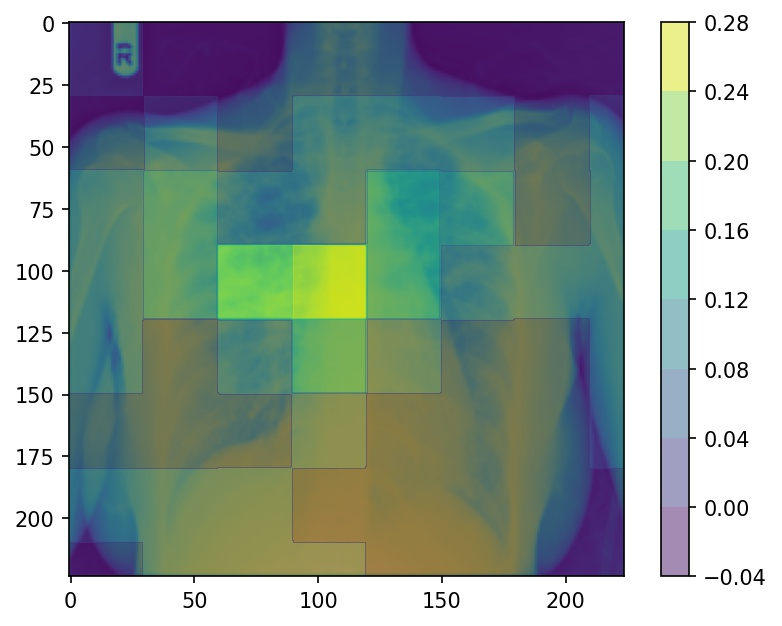
\includegraphics[width=\textwidth]{img/occlusion.jpg}
    \caption{Attribution through Occlusion}
    \label{fig:occlusion}
\end{figure}

\section{Conclusion on the Implementation}
Many of the concepts presented in \autoref{chapter:conception} were realized in the prototype, while some aspects grew to be differently than originally conceived, due to technical compromises of using Streamlit \parencite{streamlit_website}. The previous chapter gives insights on developing a flexible, multi-tier web-based application for the medical AI assessment context. The technologies used for this implementation are mainly Python and the Streamlit framework, which offer a exceptionally well match for the task at hand (see \autoref{table:software_versions}). By leveraging the data-science oriented framework, a GUI for common web browsers could be realized directly from the Python scripts working on the AI model and data. The complexities of developing a distributed web application were largely avoided - this is also reflected in the adjusted system architecture (see \autoref{fig:architecture_implementation}). However, some flexibility in implementing the conceived GUI design was lost, due to the readily provided GUI elements of Streamlit. Instead of developing custom GUI elements with a specialized frontend technology, the prepackaged elements were used. The functionalities from \autoref{section:functionalities} could all be implemented with the exception of functionality \#3. This functionality is omitted because of the failure to find a suitable algorithm to compare commonalities of X-ray images to be applied to this data set.

\newpage
\chapter{Dialogue Samples}\label{chapter:dialogue_samples}
Based on the main use case (see \autoref{section:use_cases}), the realized application will be presented in the following chapter. Leveraging a common use case, allows for an exemplary tour through the AI assessment system. The baseline is the unguided version, which gets supplemented by the guided version. Additionally mobile versions (smartphone \& tablet) will be showcased exemplarily. The application was implemented in english (shown here) and German (used for the evaluation). All versions of the application (english / German / guided / unguided) can be found digitally in \nameref{appendix:dvd_contents} or the Github repository.

\autoref{fig:samples_l_all} shows the starting point for the interaction. Opening the application in the browser leads to this landing page. The page presents the user with all functionalities in the unguided version. Alternatively the guided user gets a slightly different starting point as shown in \autoref{fig:samples_l_overview_guided}, as the guided version hides the functionalities behind the intention query on top. Following the unguided interaction flow, the user is now free to explore all functionalities by clicking on an expander GUI element. A typical starting point for the user are the first three elements as shown in \autoref{fig:samples_l_overview}. \autoref{fig:samples_l_browse} shows a possible next interaction, where the user decides to browse the AI training data. The figure highlights the focus on class-based filtering and a small sample size, that can be regenerated. The user is able to select a data point and view the image data. Additionally the user can supplement the displayed information with metadata as shown in \autoref{fig:samples_l_browse_metadata}. By opening or closing the expander elements, the user has the freedom to shape the vertical layout of the application. Closing the other elements allows for a better overview and navigation as shown in \autoref{fig:samples_l_experiment}, while focusing on the current functionality. The input-output experiment may be a interesting next interaction point for the user, because it was commonly requested as described in \autoref{section:user_analysis}. To further deepen the understanding of the AI, the user might want to see how the AI came to its results. \autoref{fig:samples_l_experiment_occlusion} shows the visual explanation method (see \autoref{subsection:explanation_techniques}), which the user can use to gain additional information about the AI's reasoning. \autoref{fig:samples_l_experiment_guided} shows the alternative guided experiment functionality for comparison. Finally the user might want to explore some more detailed information about the data set and therefore go to the data clustering functionality as depicted by \autoref{fig:samples_l_data_cluster}, where the user can gain insights about statistical patterns recognized in the meta data. Although not all functionalities were used, such can be a exemplary user scenario. Furthermore the application is designed to be responsive in regards to the used device. \autoref{fig:samples_m_limits} shows the previously omitted model limitations functionality on a medium sized device, such as a tablet. Using such a device has the advantage of a possible vertical screen orientation and therefore being able to present more information vertically. \autoref{fig:samples_m_experiment} supports this statement, where the user can interact with the whole experiment functionality in contrast to \autoref{fig:samples_l_experiment}. However further reducing the screen size leads to a cluttered interface: \autoref{fig:samples_s_overview_metrics} and \autoref{fig:samples_s_experiment_browse} show the overview, metrics, browse and experiment functionality on a smartphone.

\begin{figure}[htbp]
    \centering
    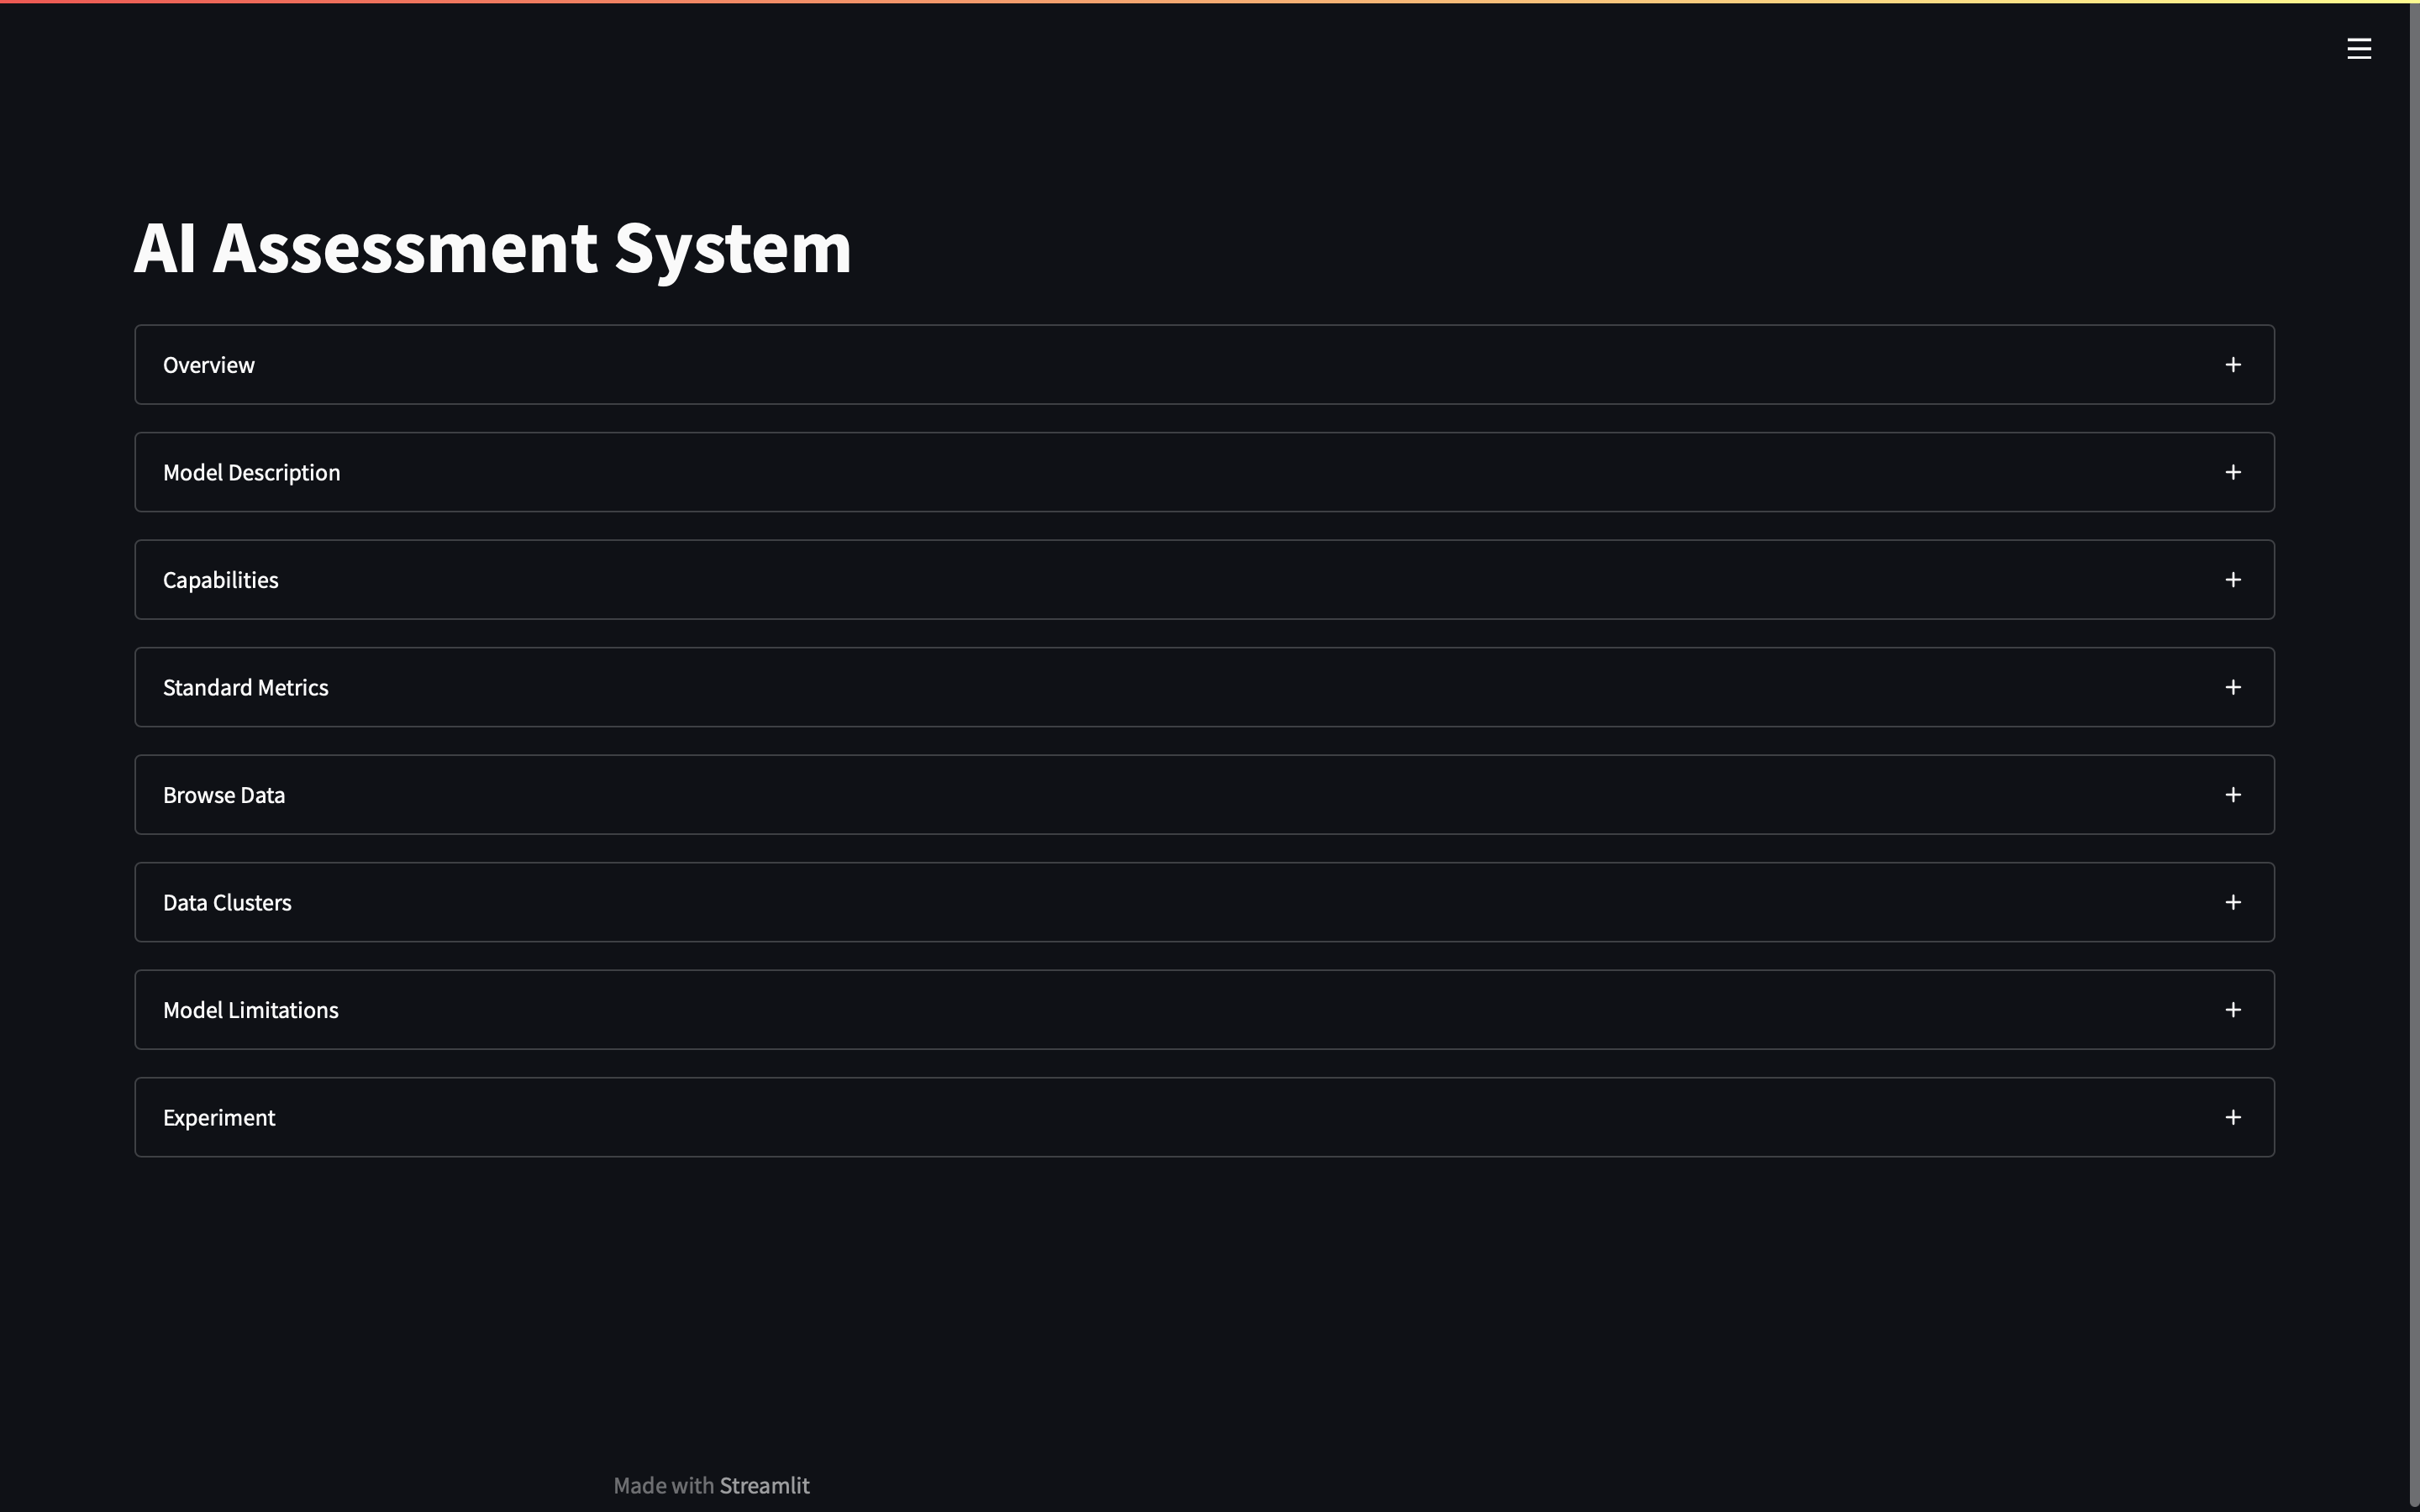
\includegraphics[width=\textwidth]{img/screenshots/samples/large/l_all.png}
    \caption{Dialogue Sample - All Functionalities (large display)}
    \label{fig:samples_l_all}
\end{figure}

\begin{figure}[htbp]
    \centering
    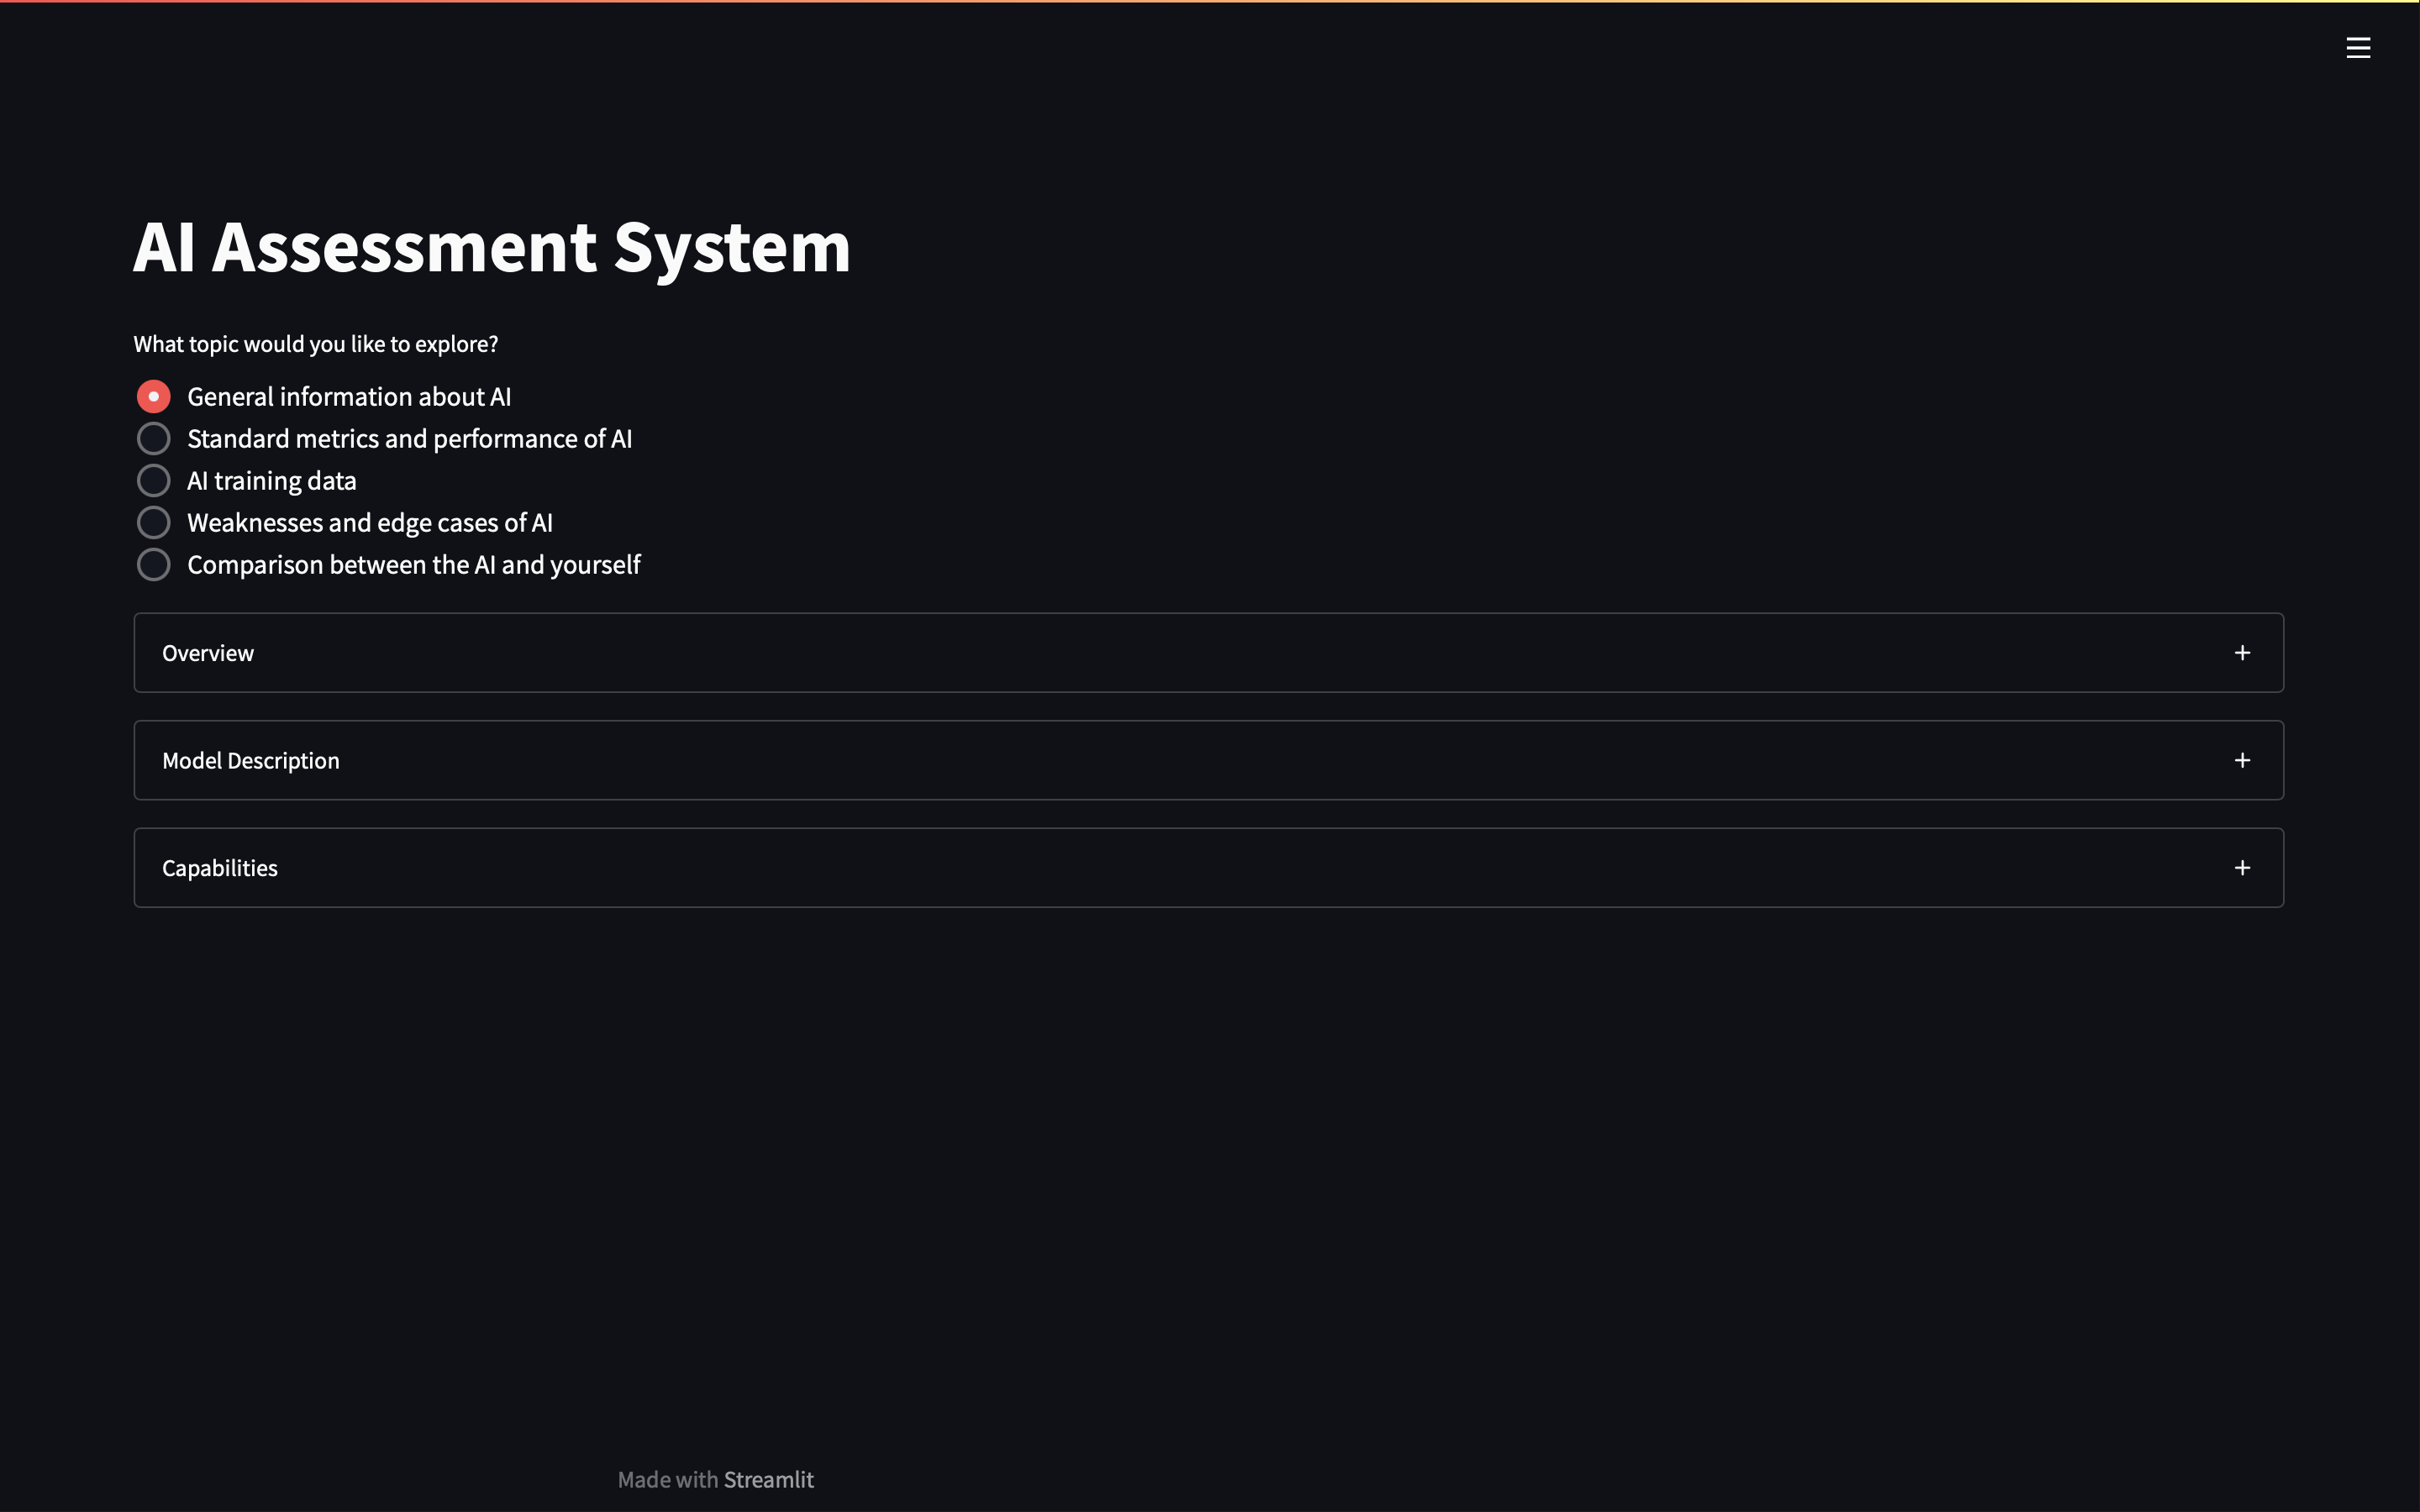
\includegraphics[width=\textwidth]{img/screenshots/samples/large/l_overview_guided.png}
    \caption{Dialogue Sample - Guided Overview Functionalities (large display)}
    \label{fig:samples_l_overview_guided}
\end{figure}

\begin{figure}[htbp]
    \centering
    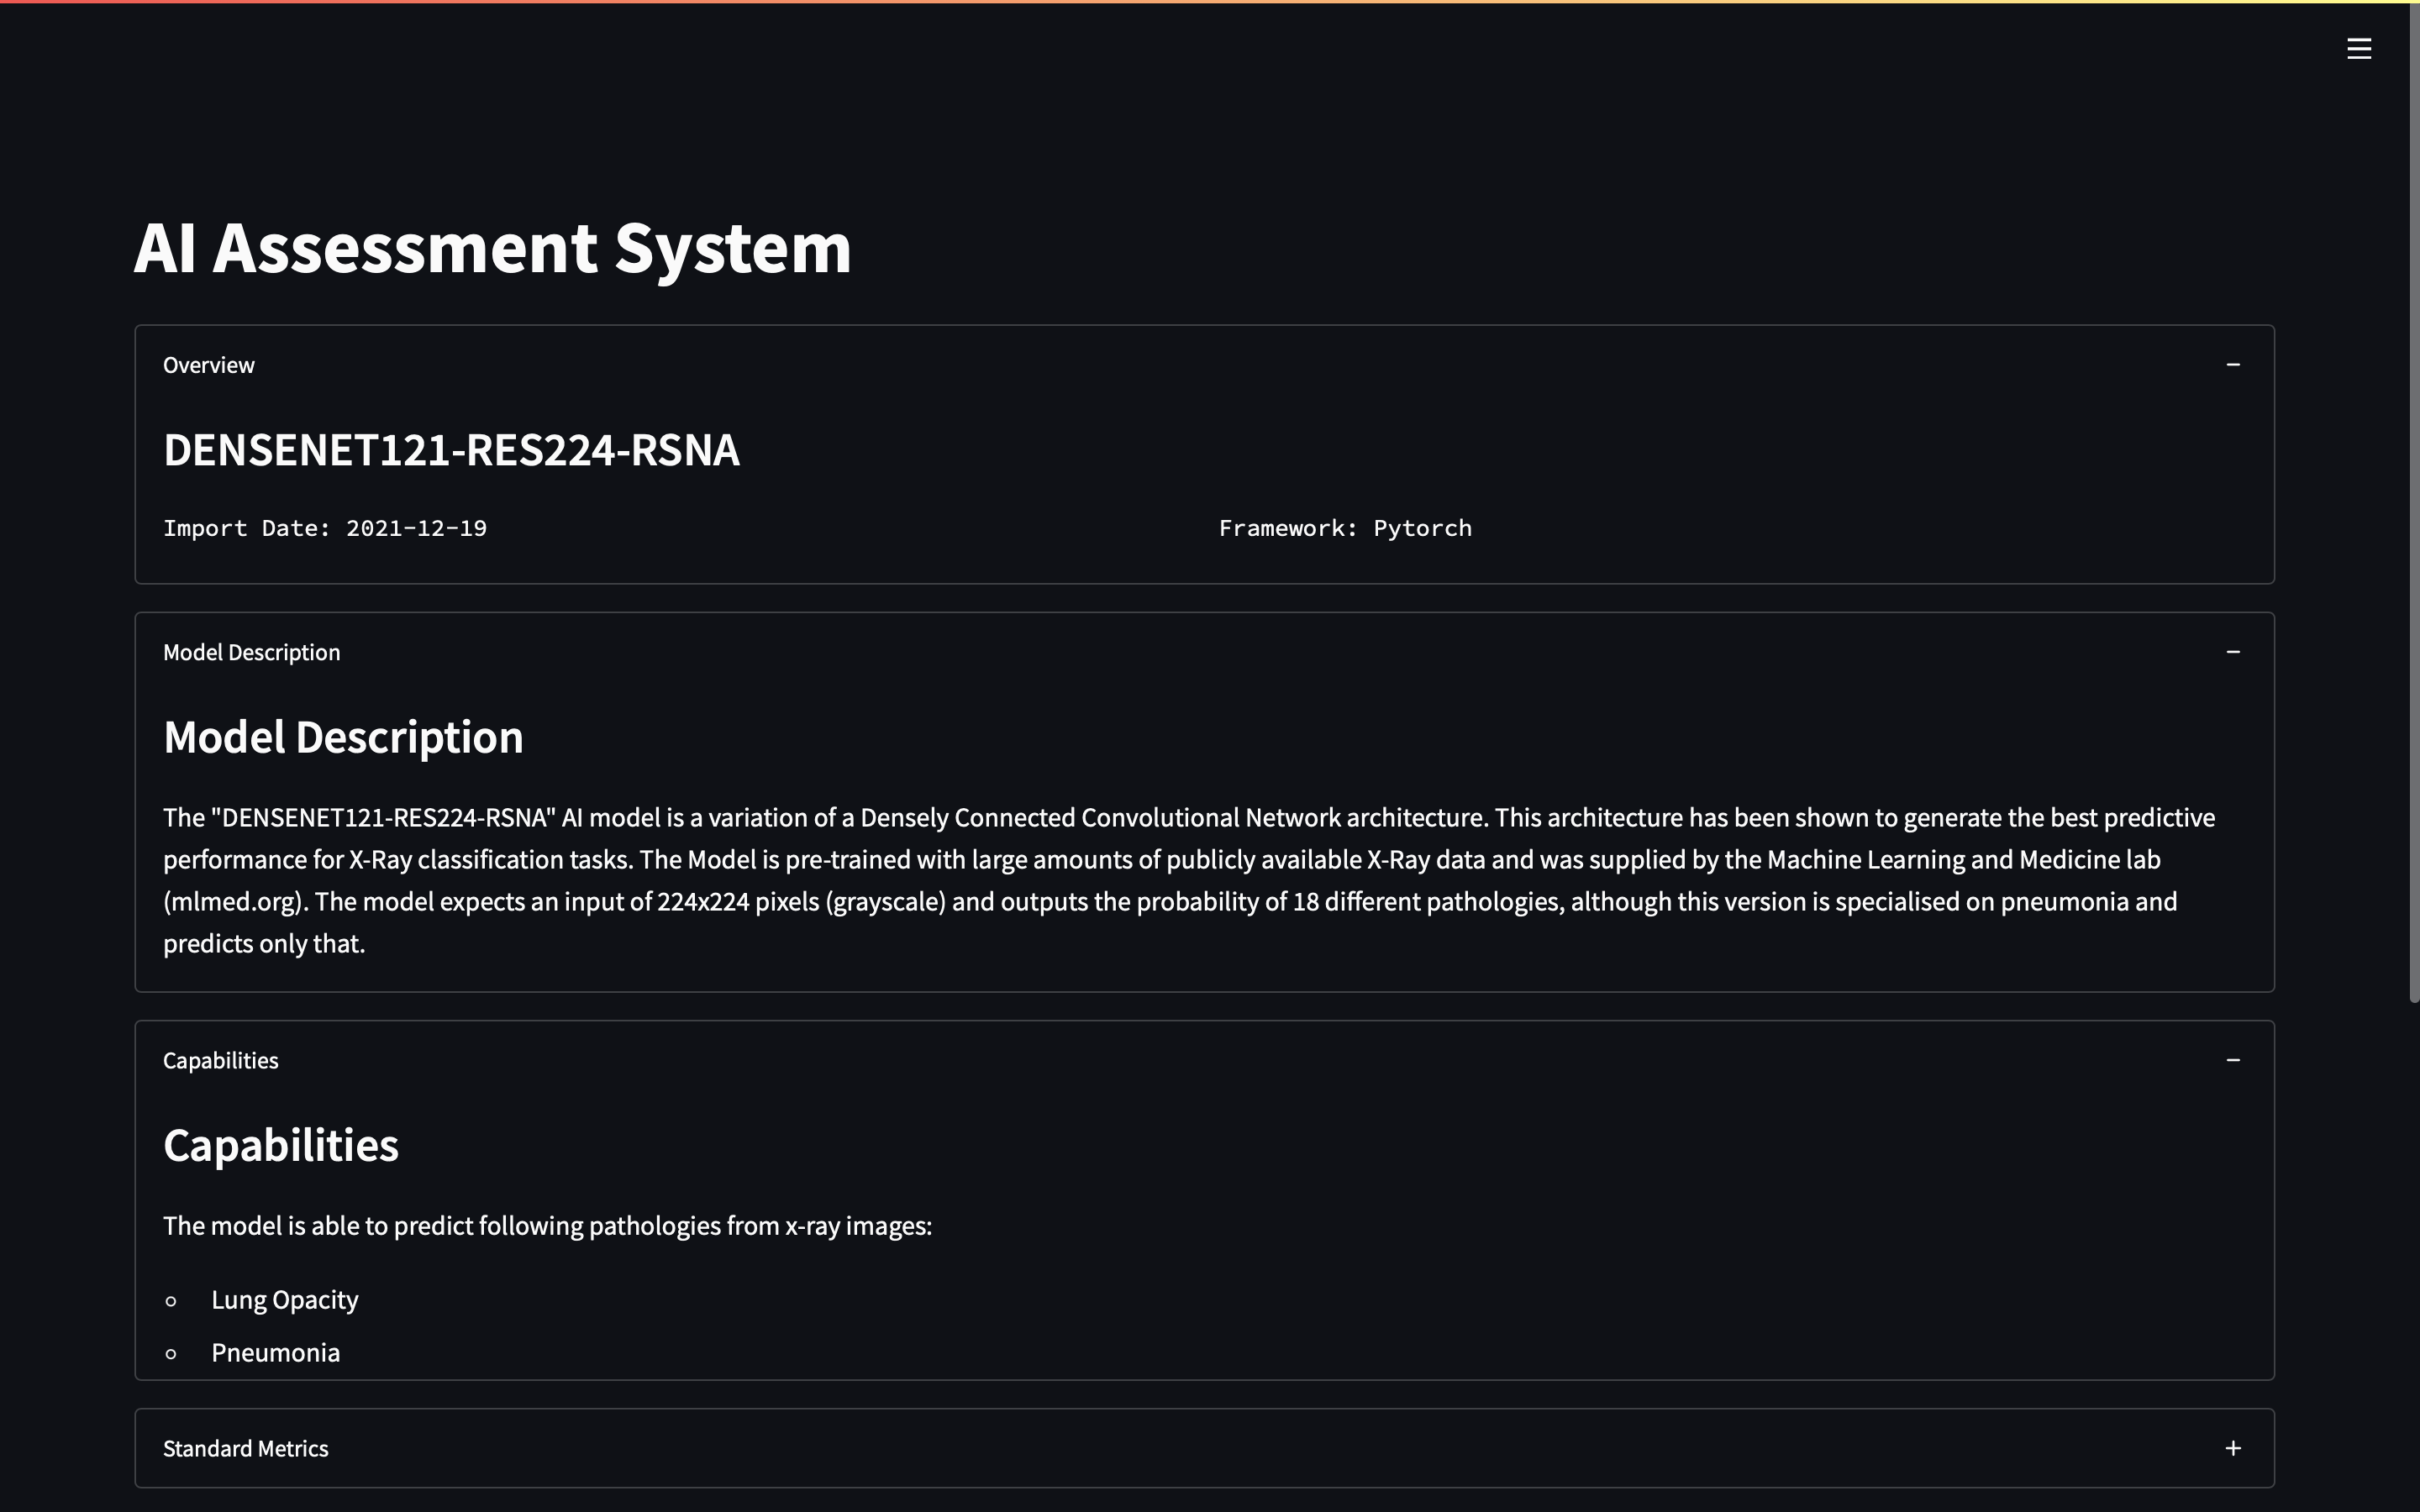
\includegraphics[width=\textwidth]{img/screenshots/samples/large/l_overview.png}
    \caption{Dialogue Sample - Overview Functionalities (large display)}
    \label{fig:samples_l_overview}
\end{figure}

\begin{figure}[htbp]
    \centering
    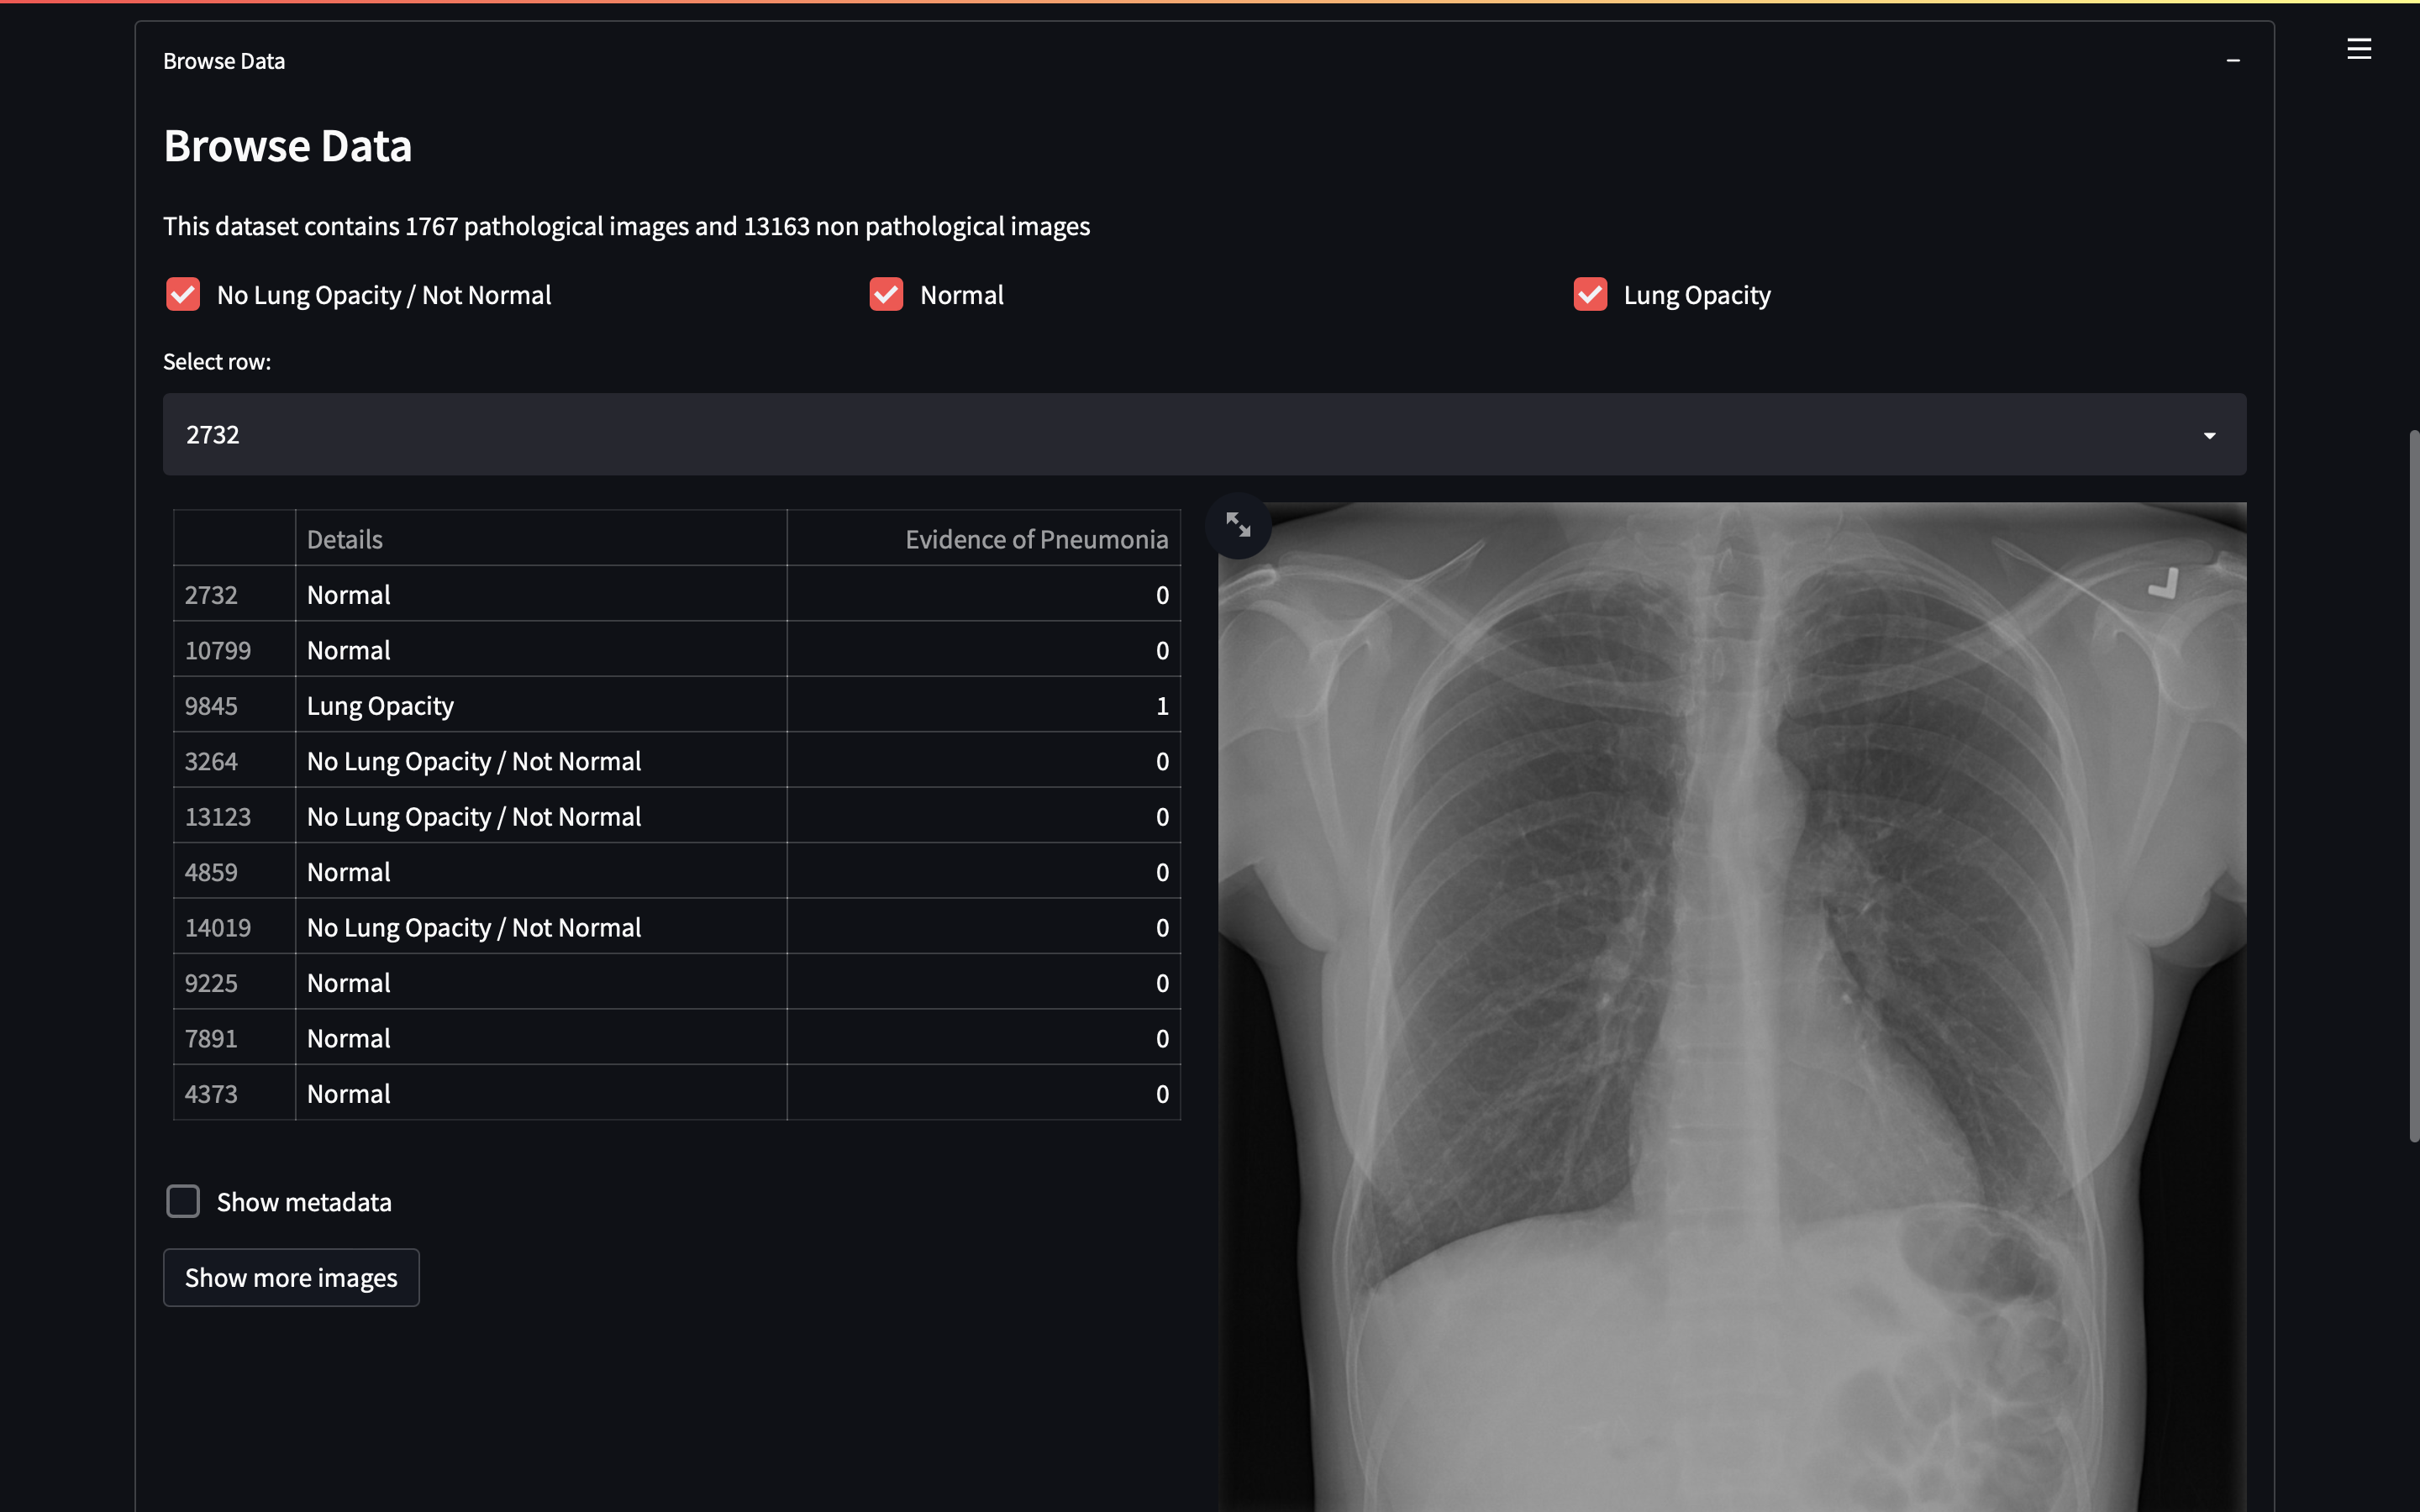
\includegraphics[width=\textwidth]{img/screenshots/samples/large/l_browse.png}
    \caption{Dialogue Sample - Browse Functionality (large display)}
    \label{fig:samples_l_browse}
\end{figure}

\begin{figure}[htbp]
    \centering
    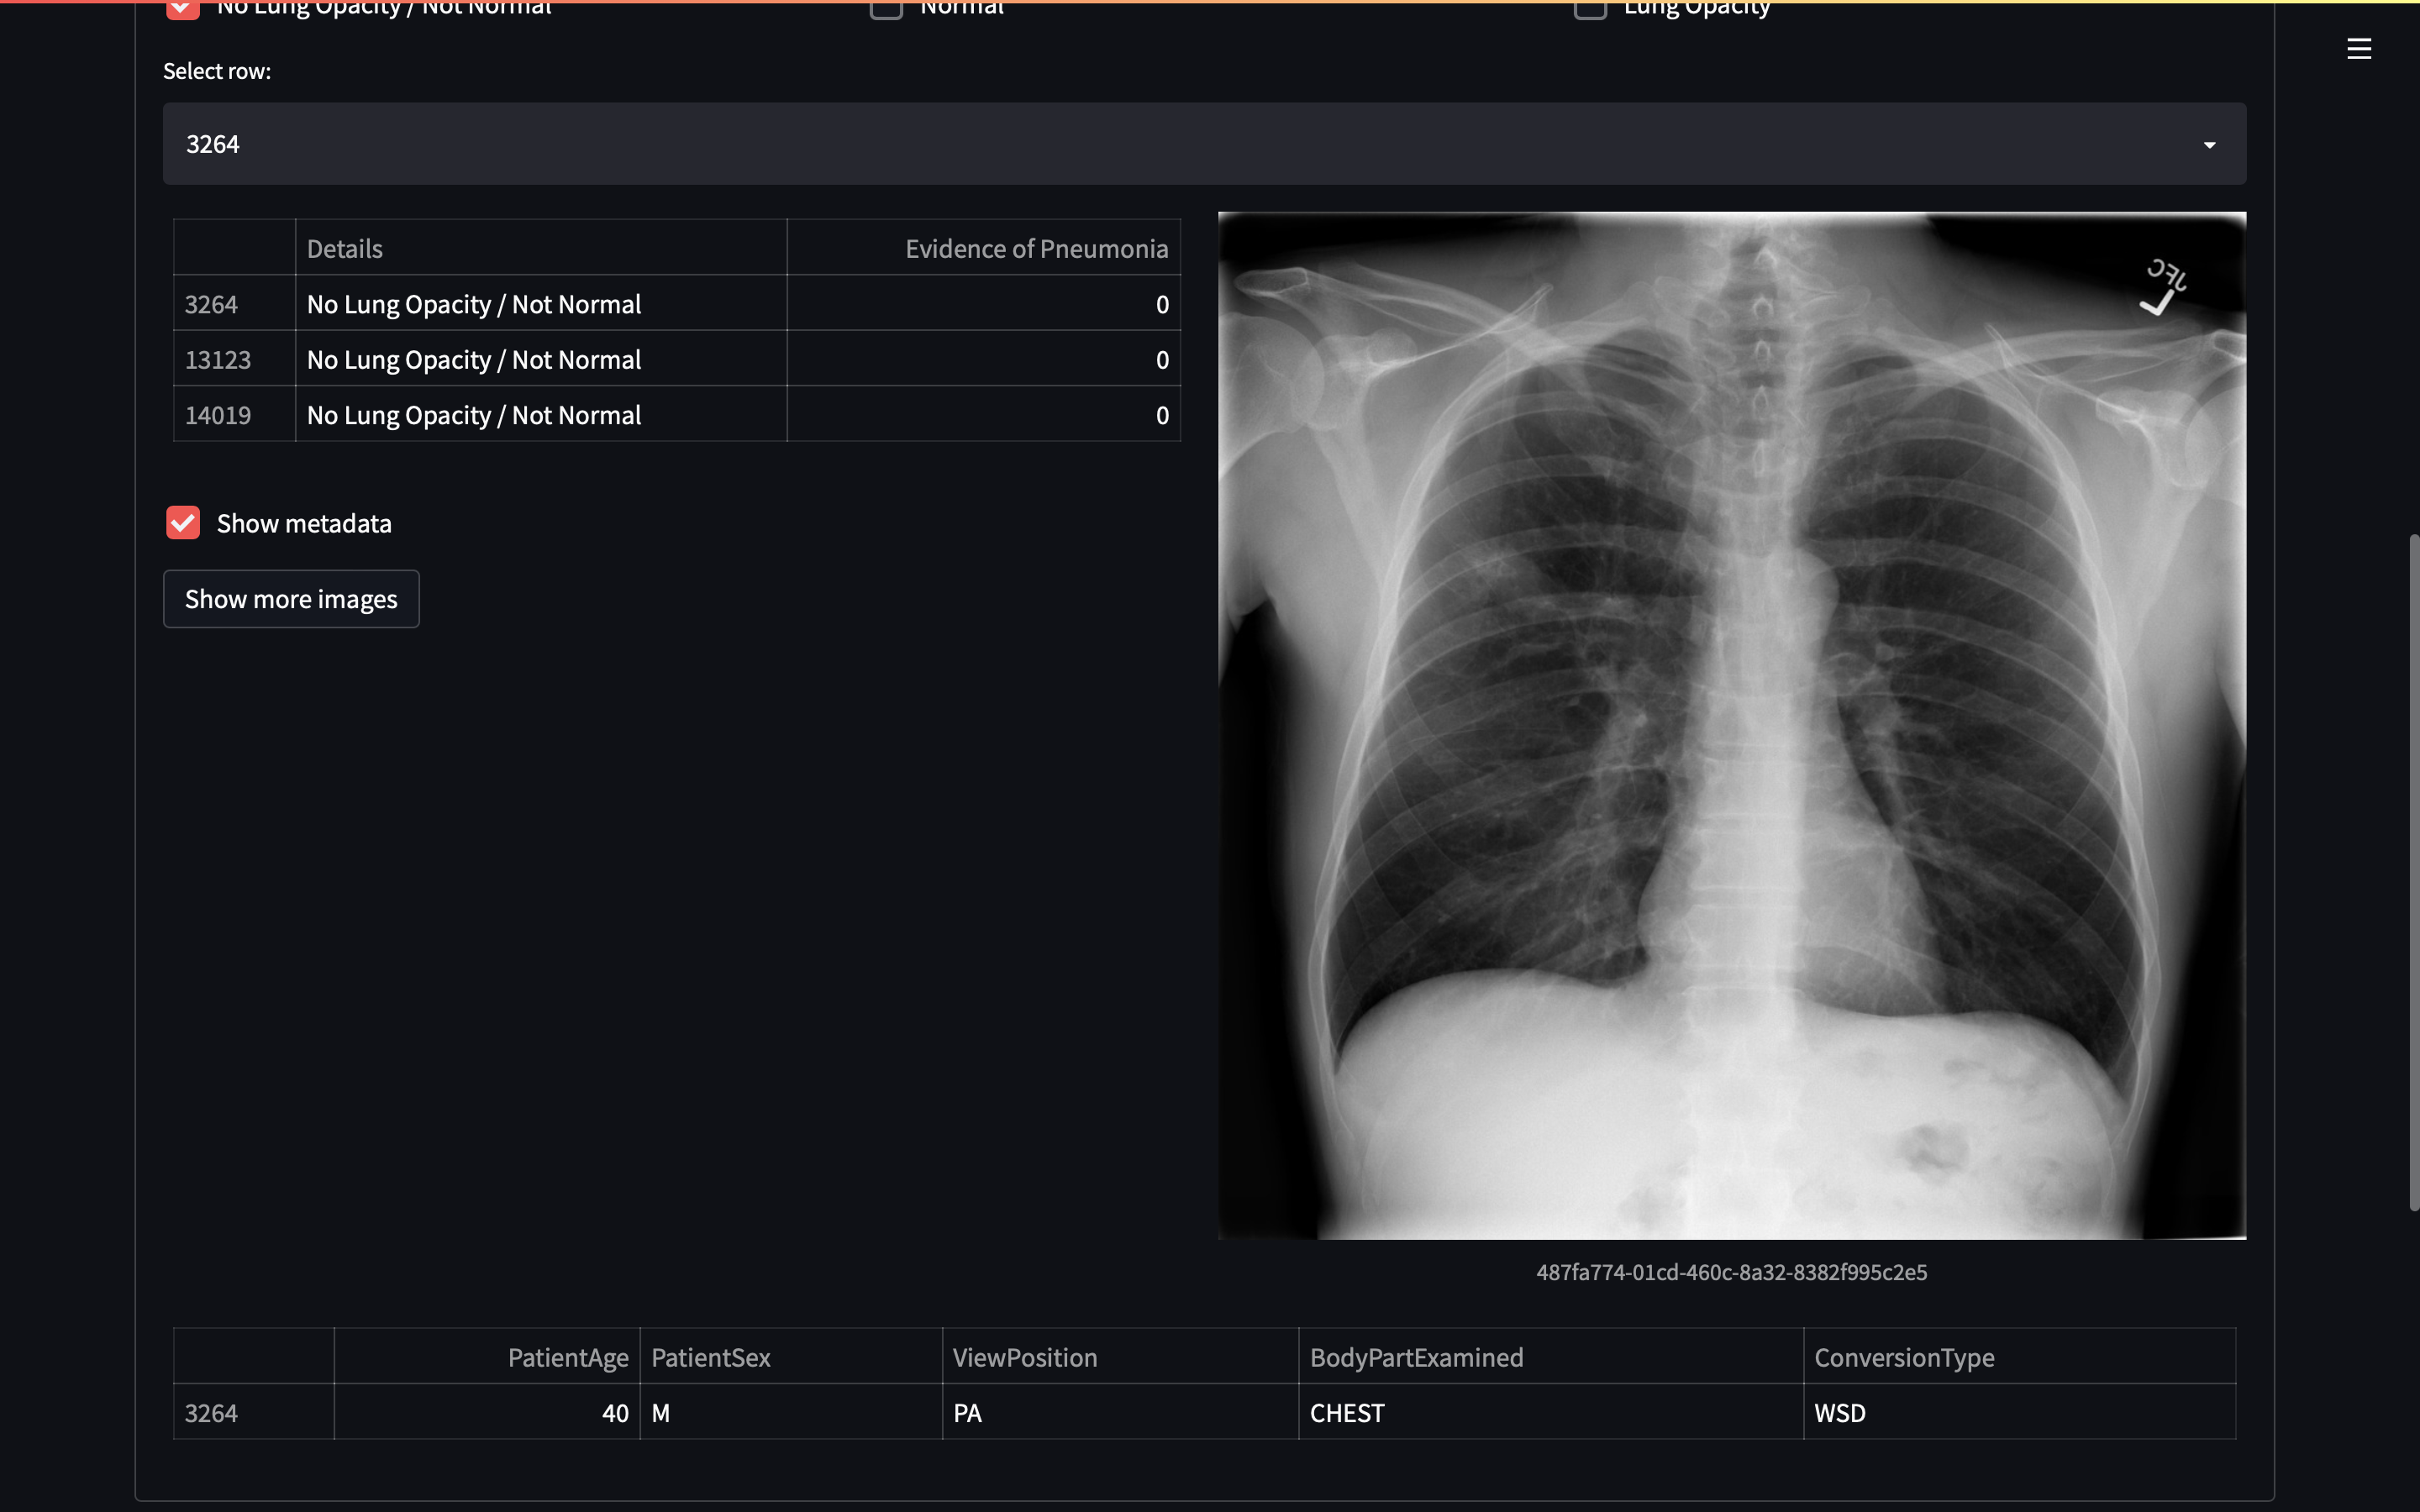
\includegraphics[width=\textwidth]{img/screenshots/samples/large/l_browse_metadata.png}
    \caption{Dialogue Sample - Browse Functionality with Metadata (large display)}
    \label{fig:samples_l_browse_metadata}
\end{figure}

\begin{figure}[htbp]
    \centering
    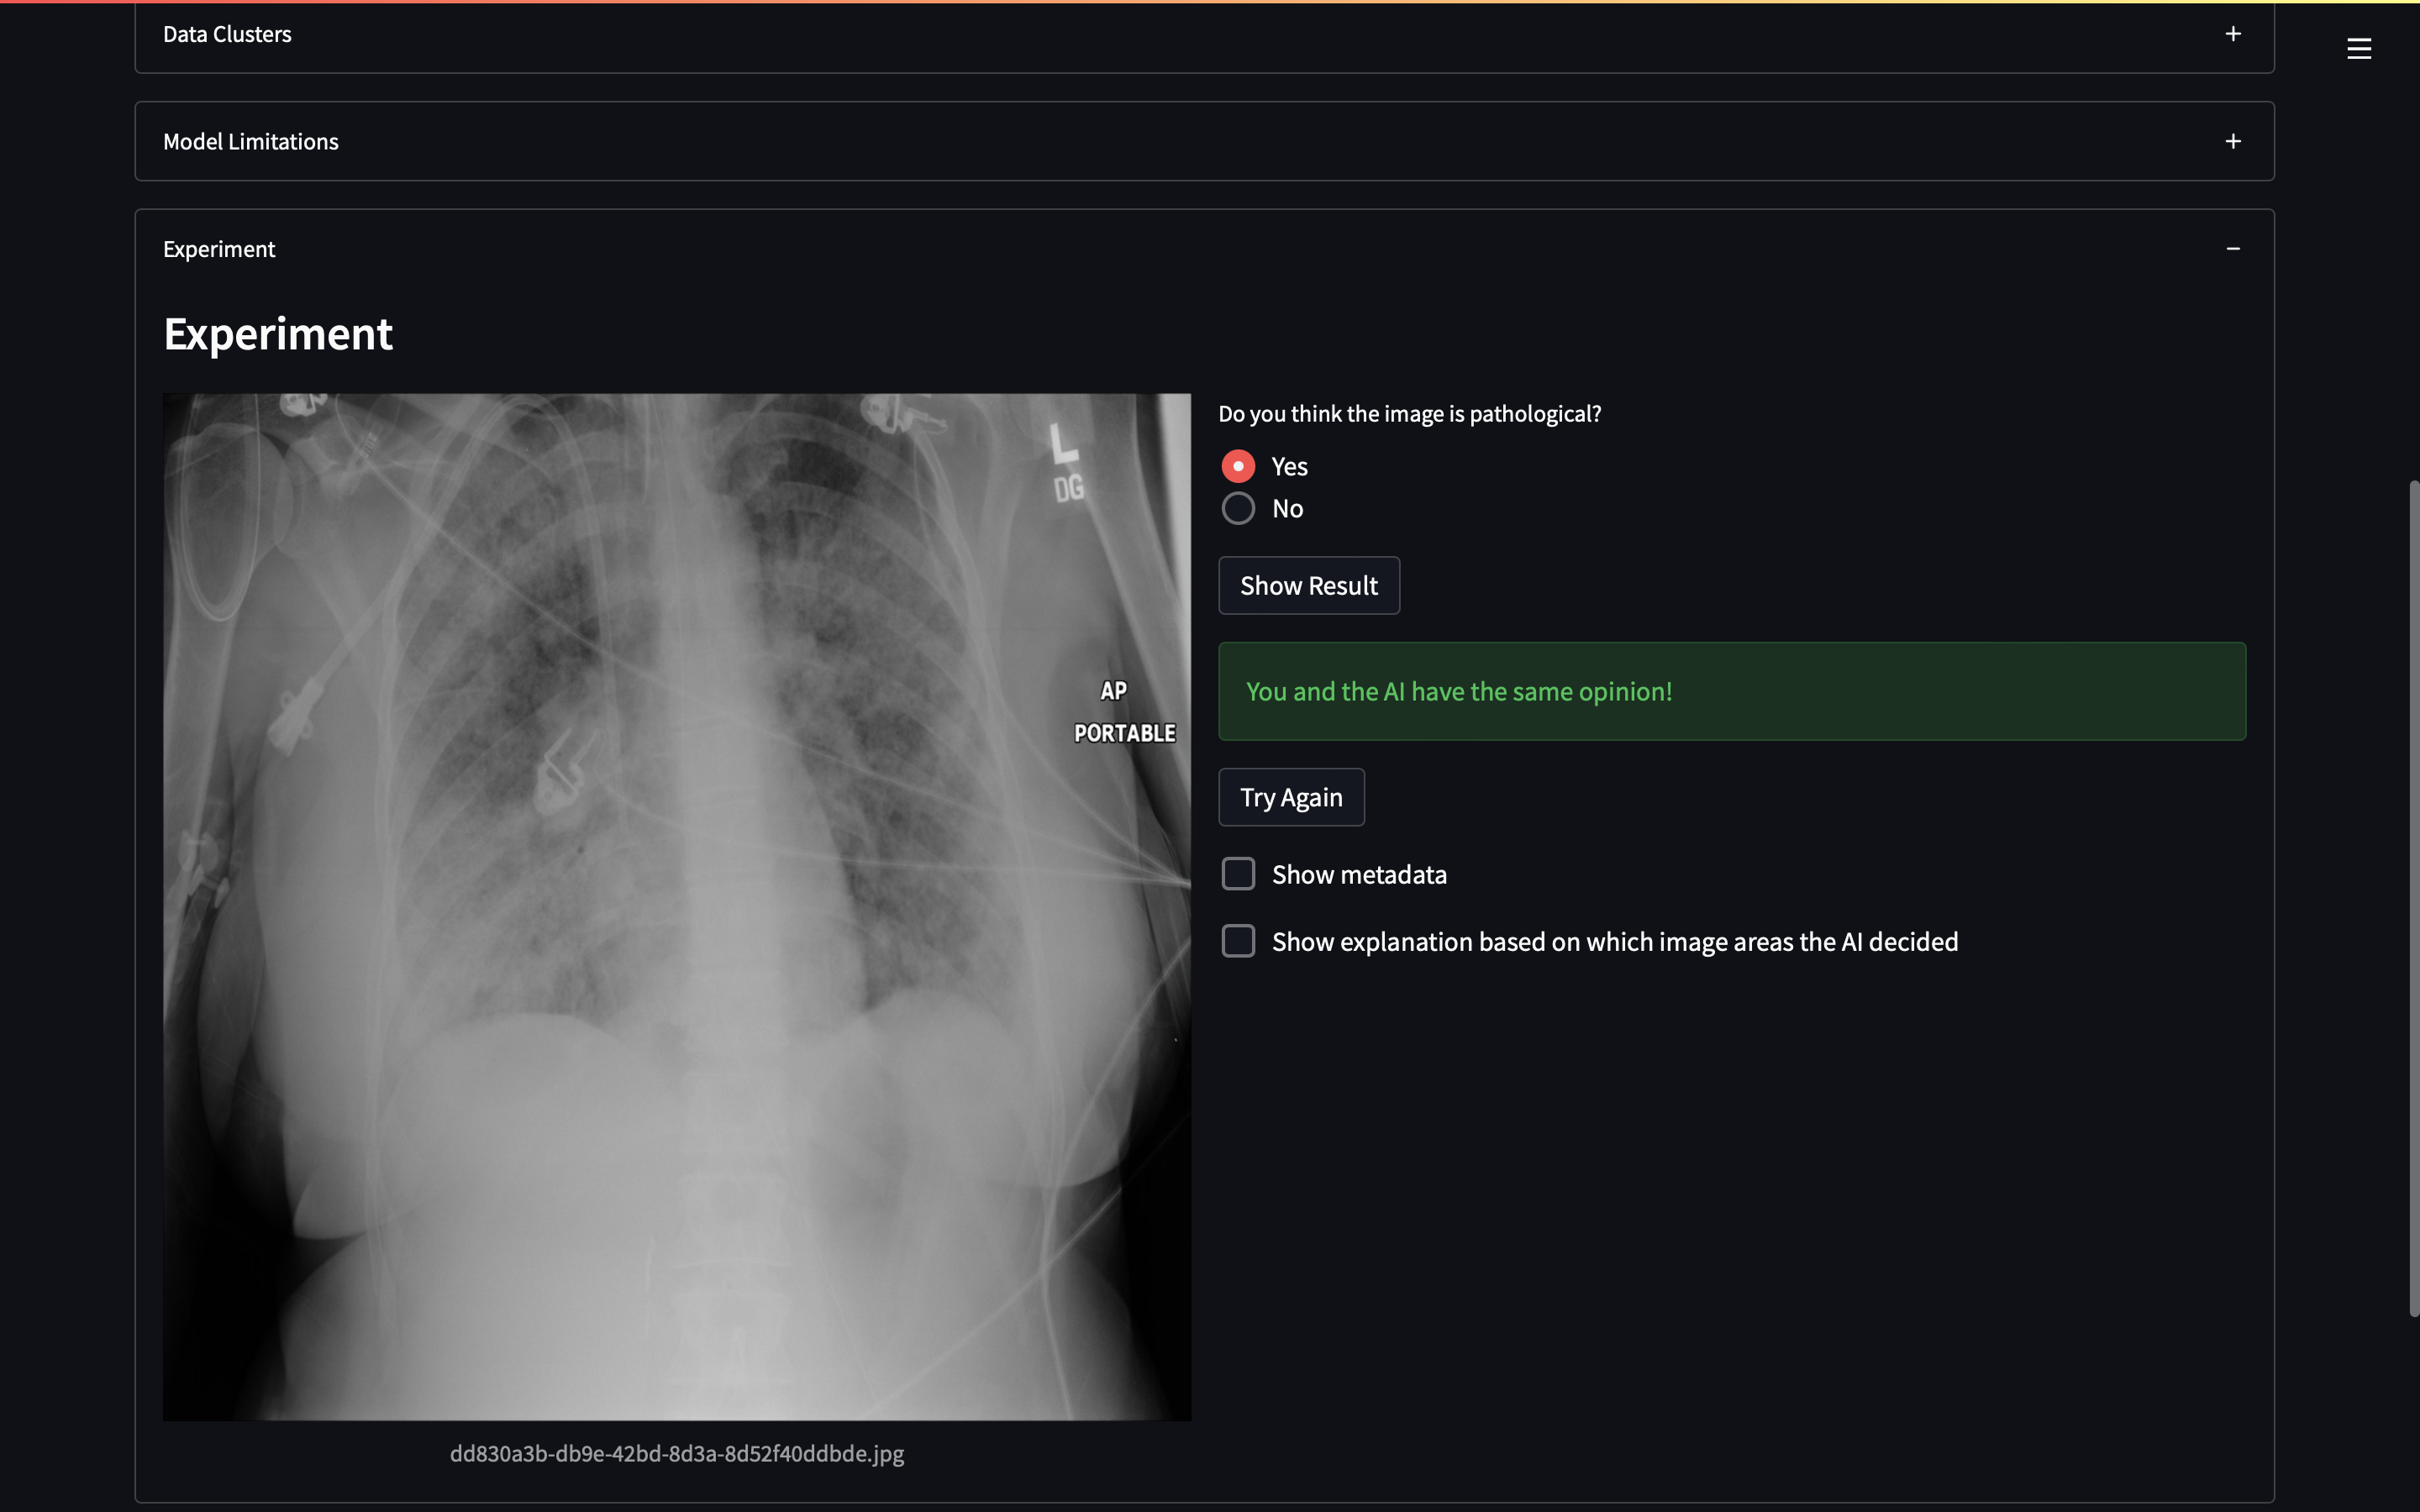
\includegraphics[width=\textwidth]{img/screenshots/samples/large/l_experiment.png}
    \caption{Dialogue Sample - Experiment Functionality (large display)}
    \label{fig:samples_l_experiment}
\end{figure}

\begin{figure}[htbp]
    \centering
    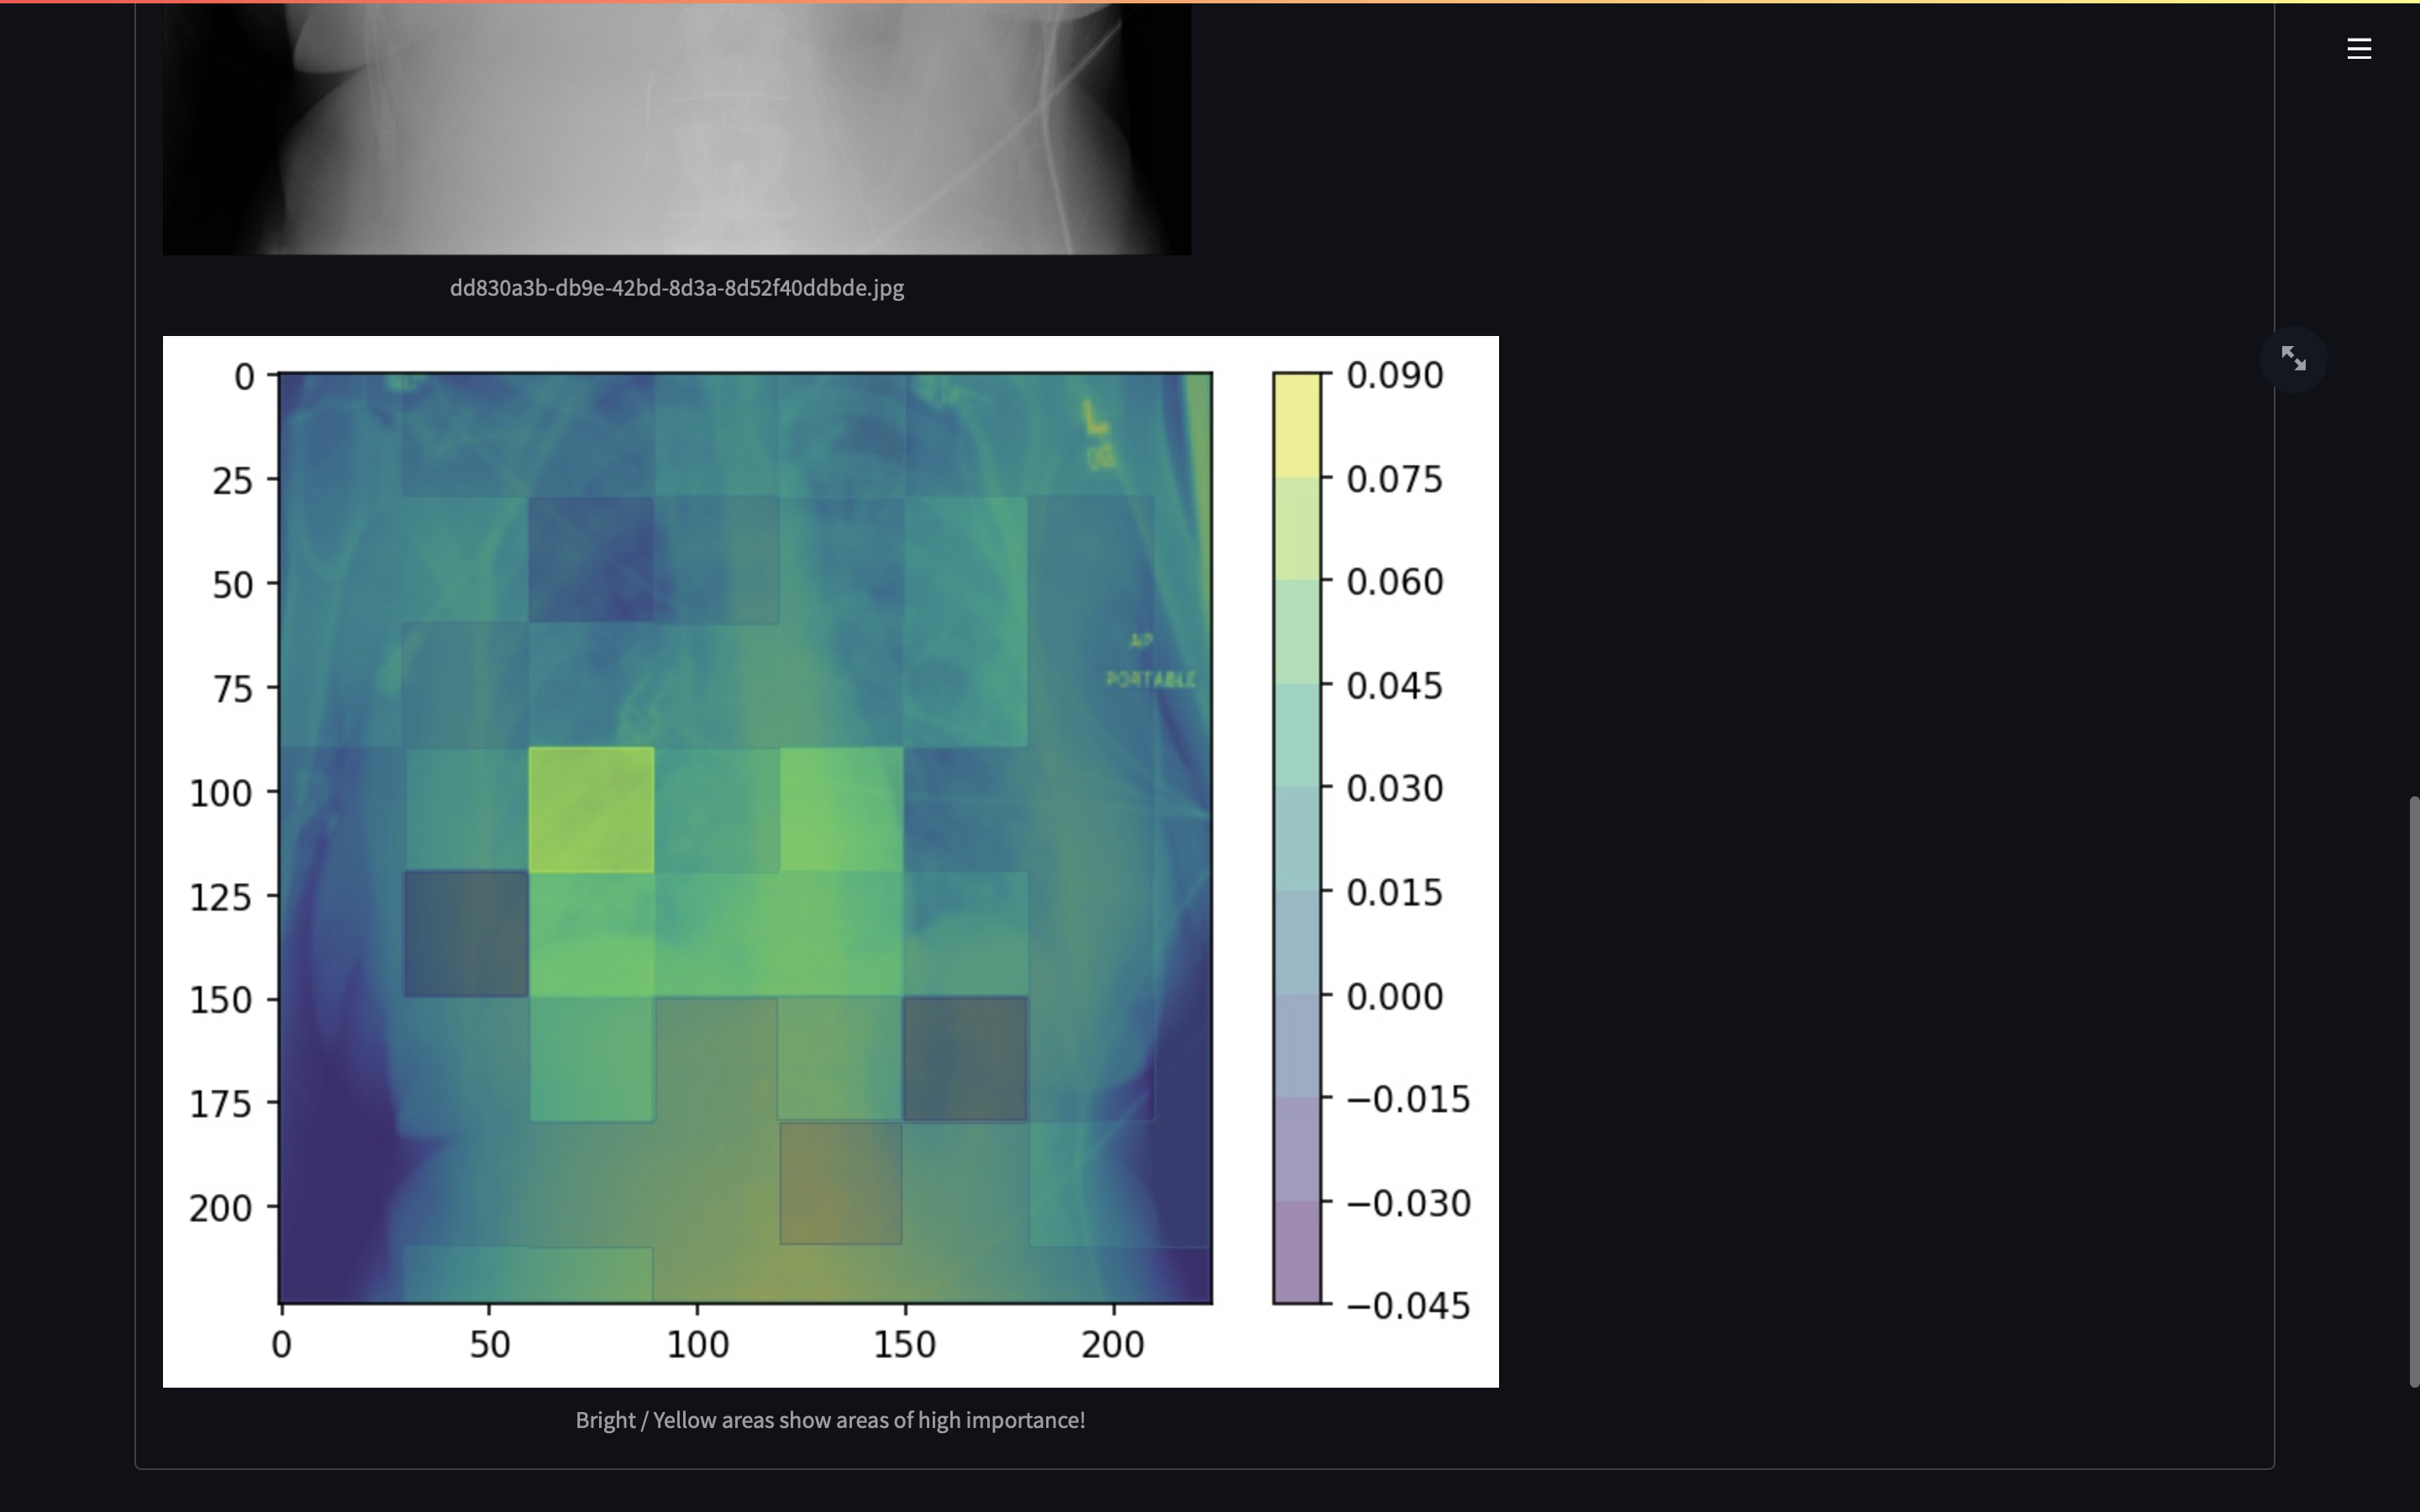
\includegraphics[width=\textwidth]{img/screenshots/samples/large/l_experiment_occlusion.png}
    \caption{Dialogue Sample - Experiment Functionality with Attribution by Occlusion (large display)}
    \label{fig:samples_l_experiment_occlusion}
\end{figure}

\begin{figure}[htbp]
    \centering
    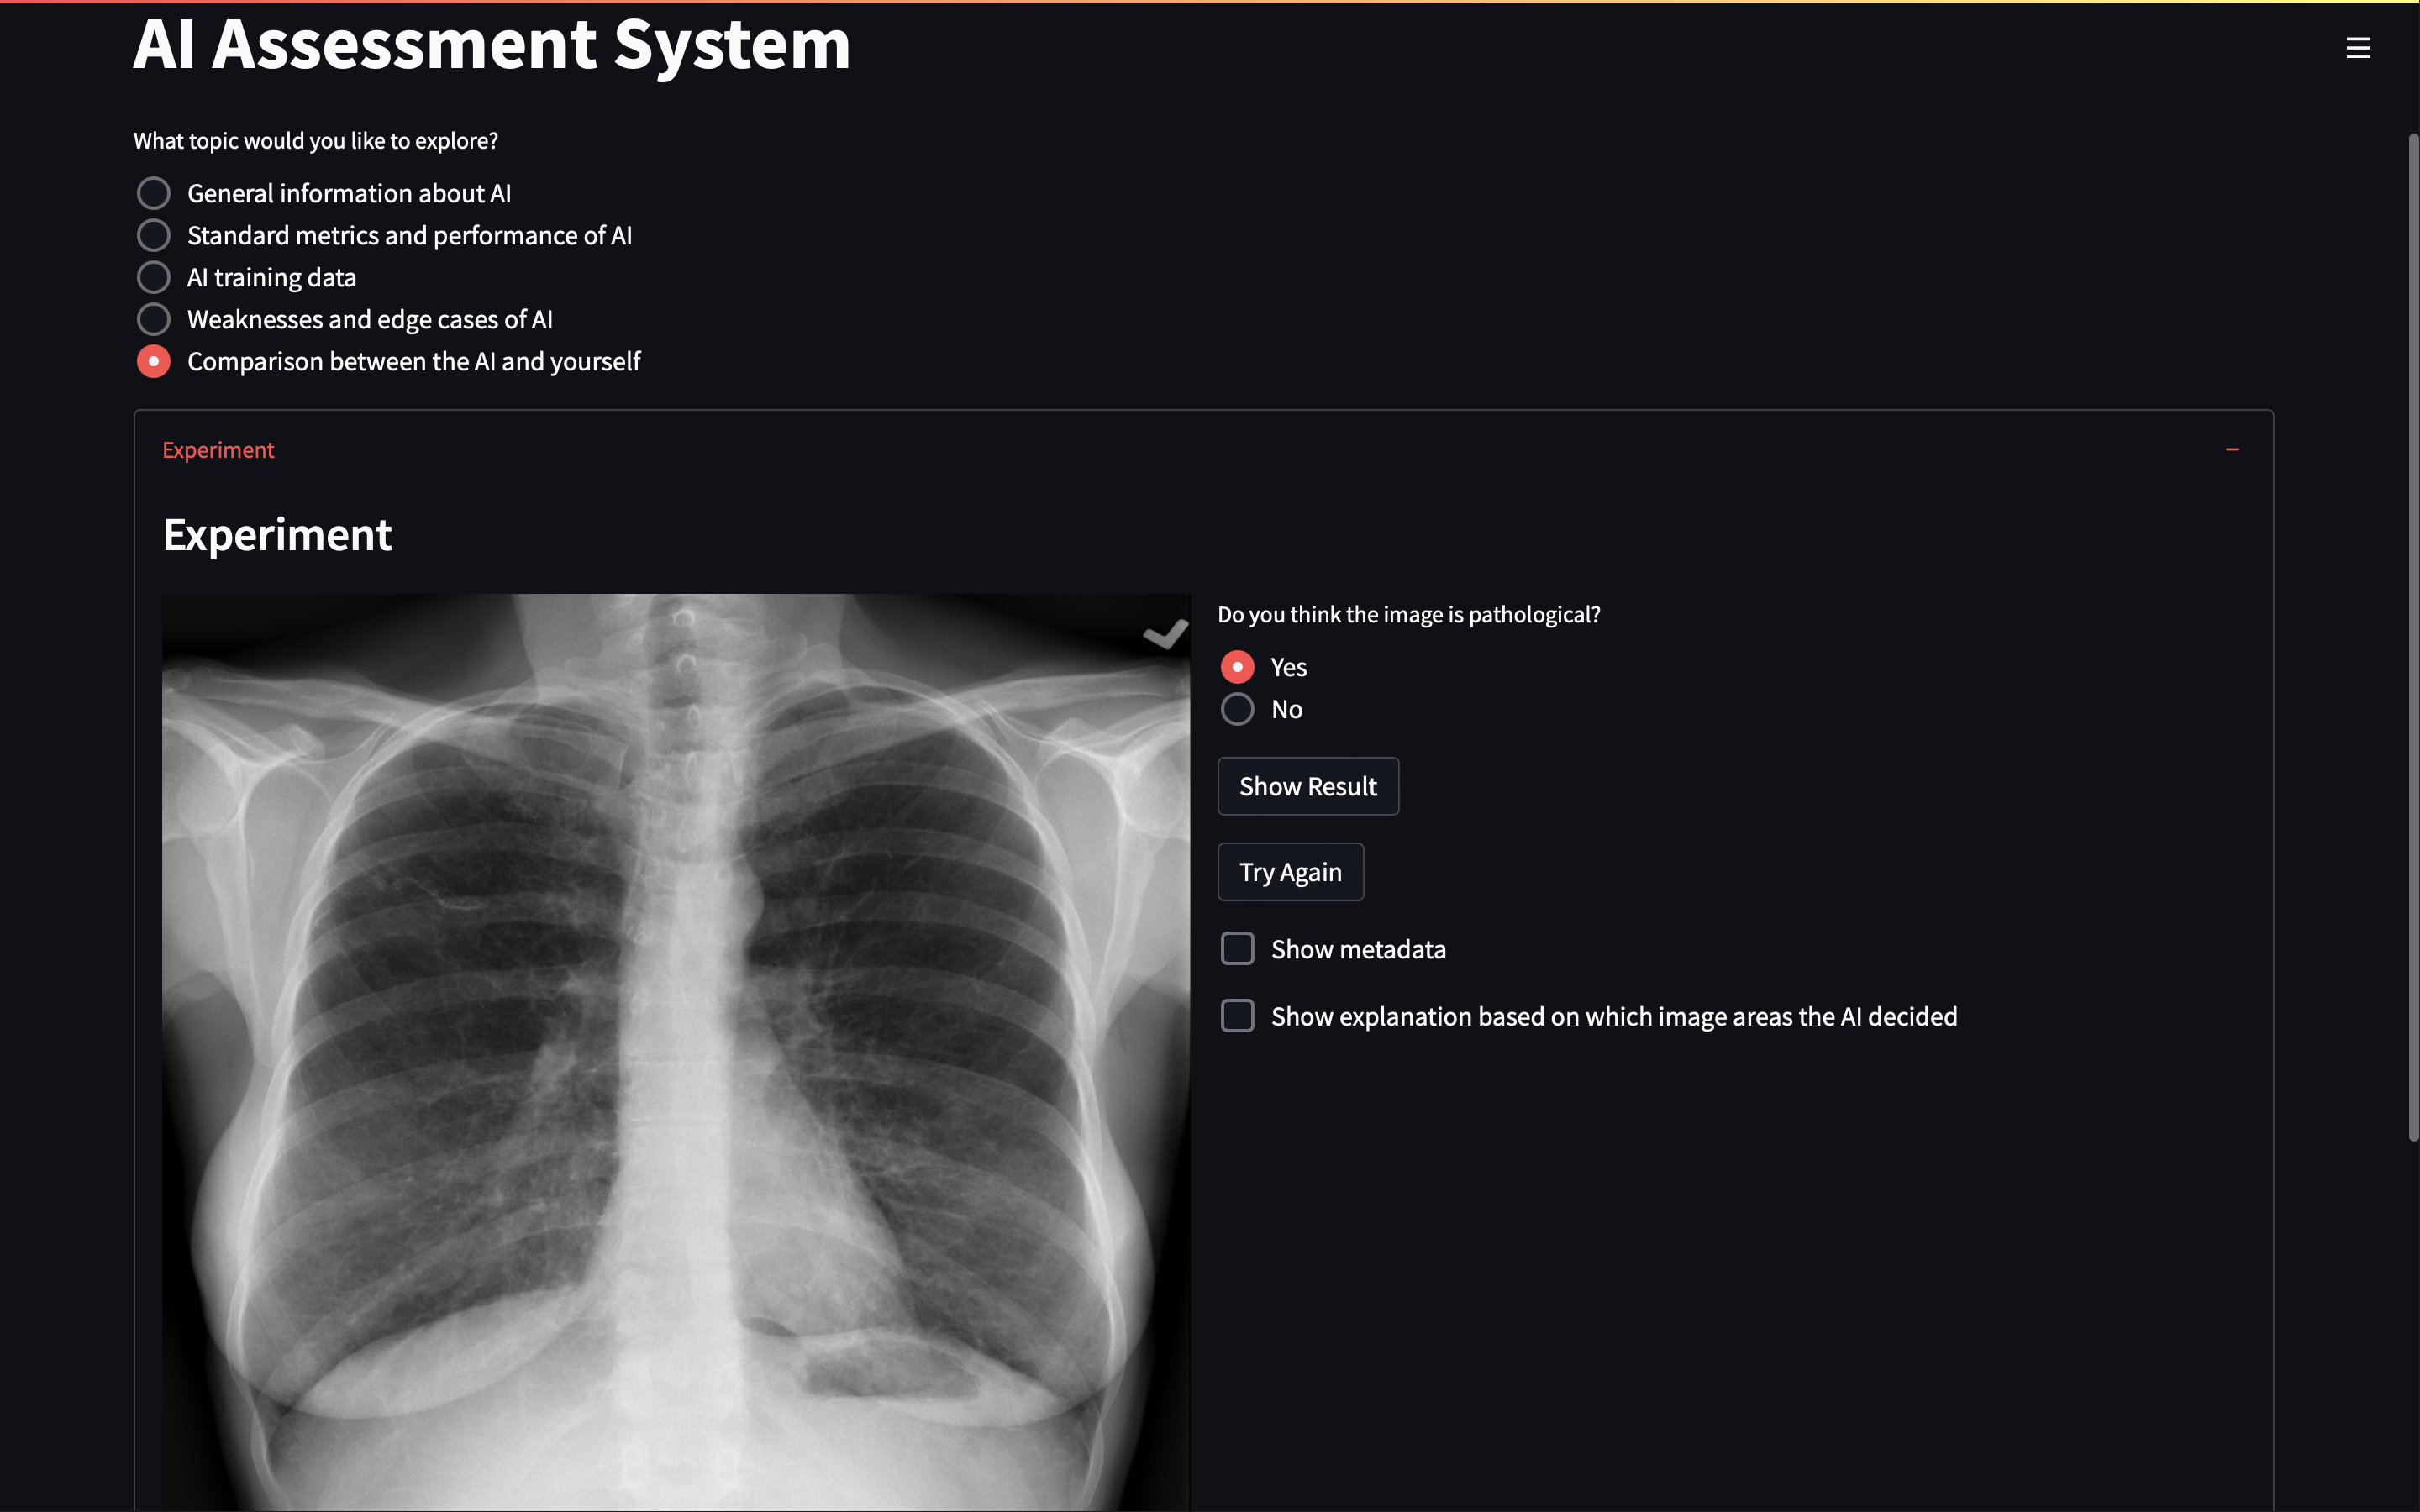
\includegraphics[width=\textwidth]{img/screenshots/samples/large/l_experiment_guided_active.png}
    \caption{Dialogue Sample - Guided Experiment Functionality (large display)}
    \label{fig:samples_l_experiment_guided}
\end{figure}

\begin{figure}[htbp]
    \centering
    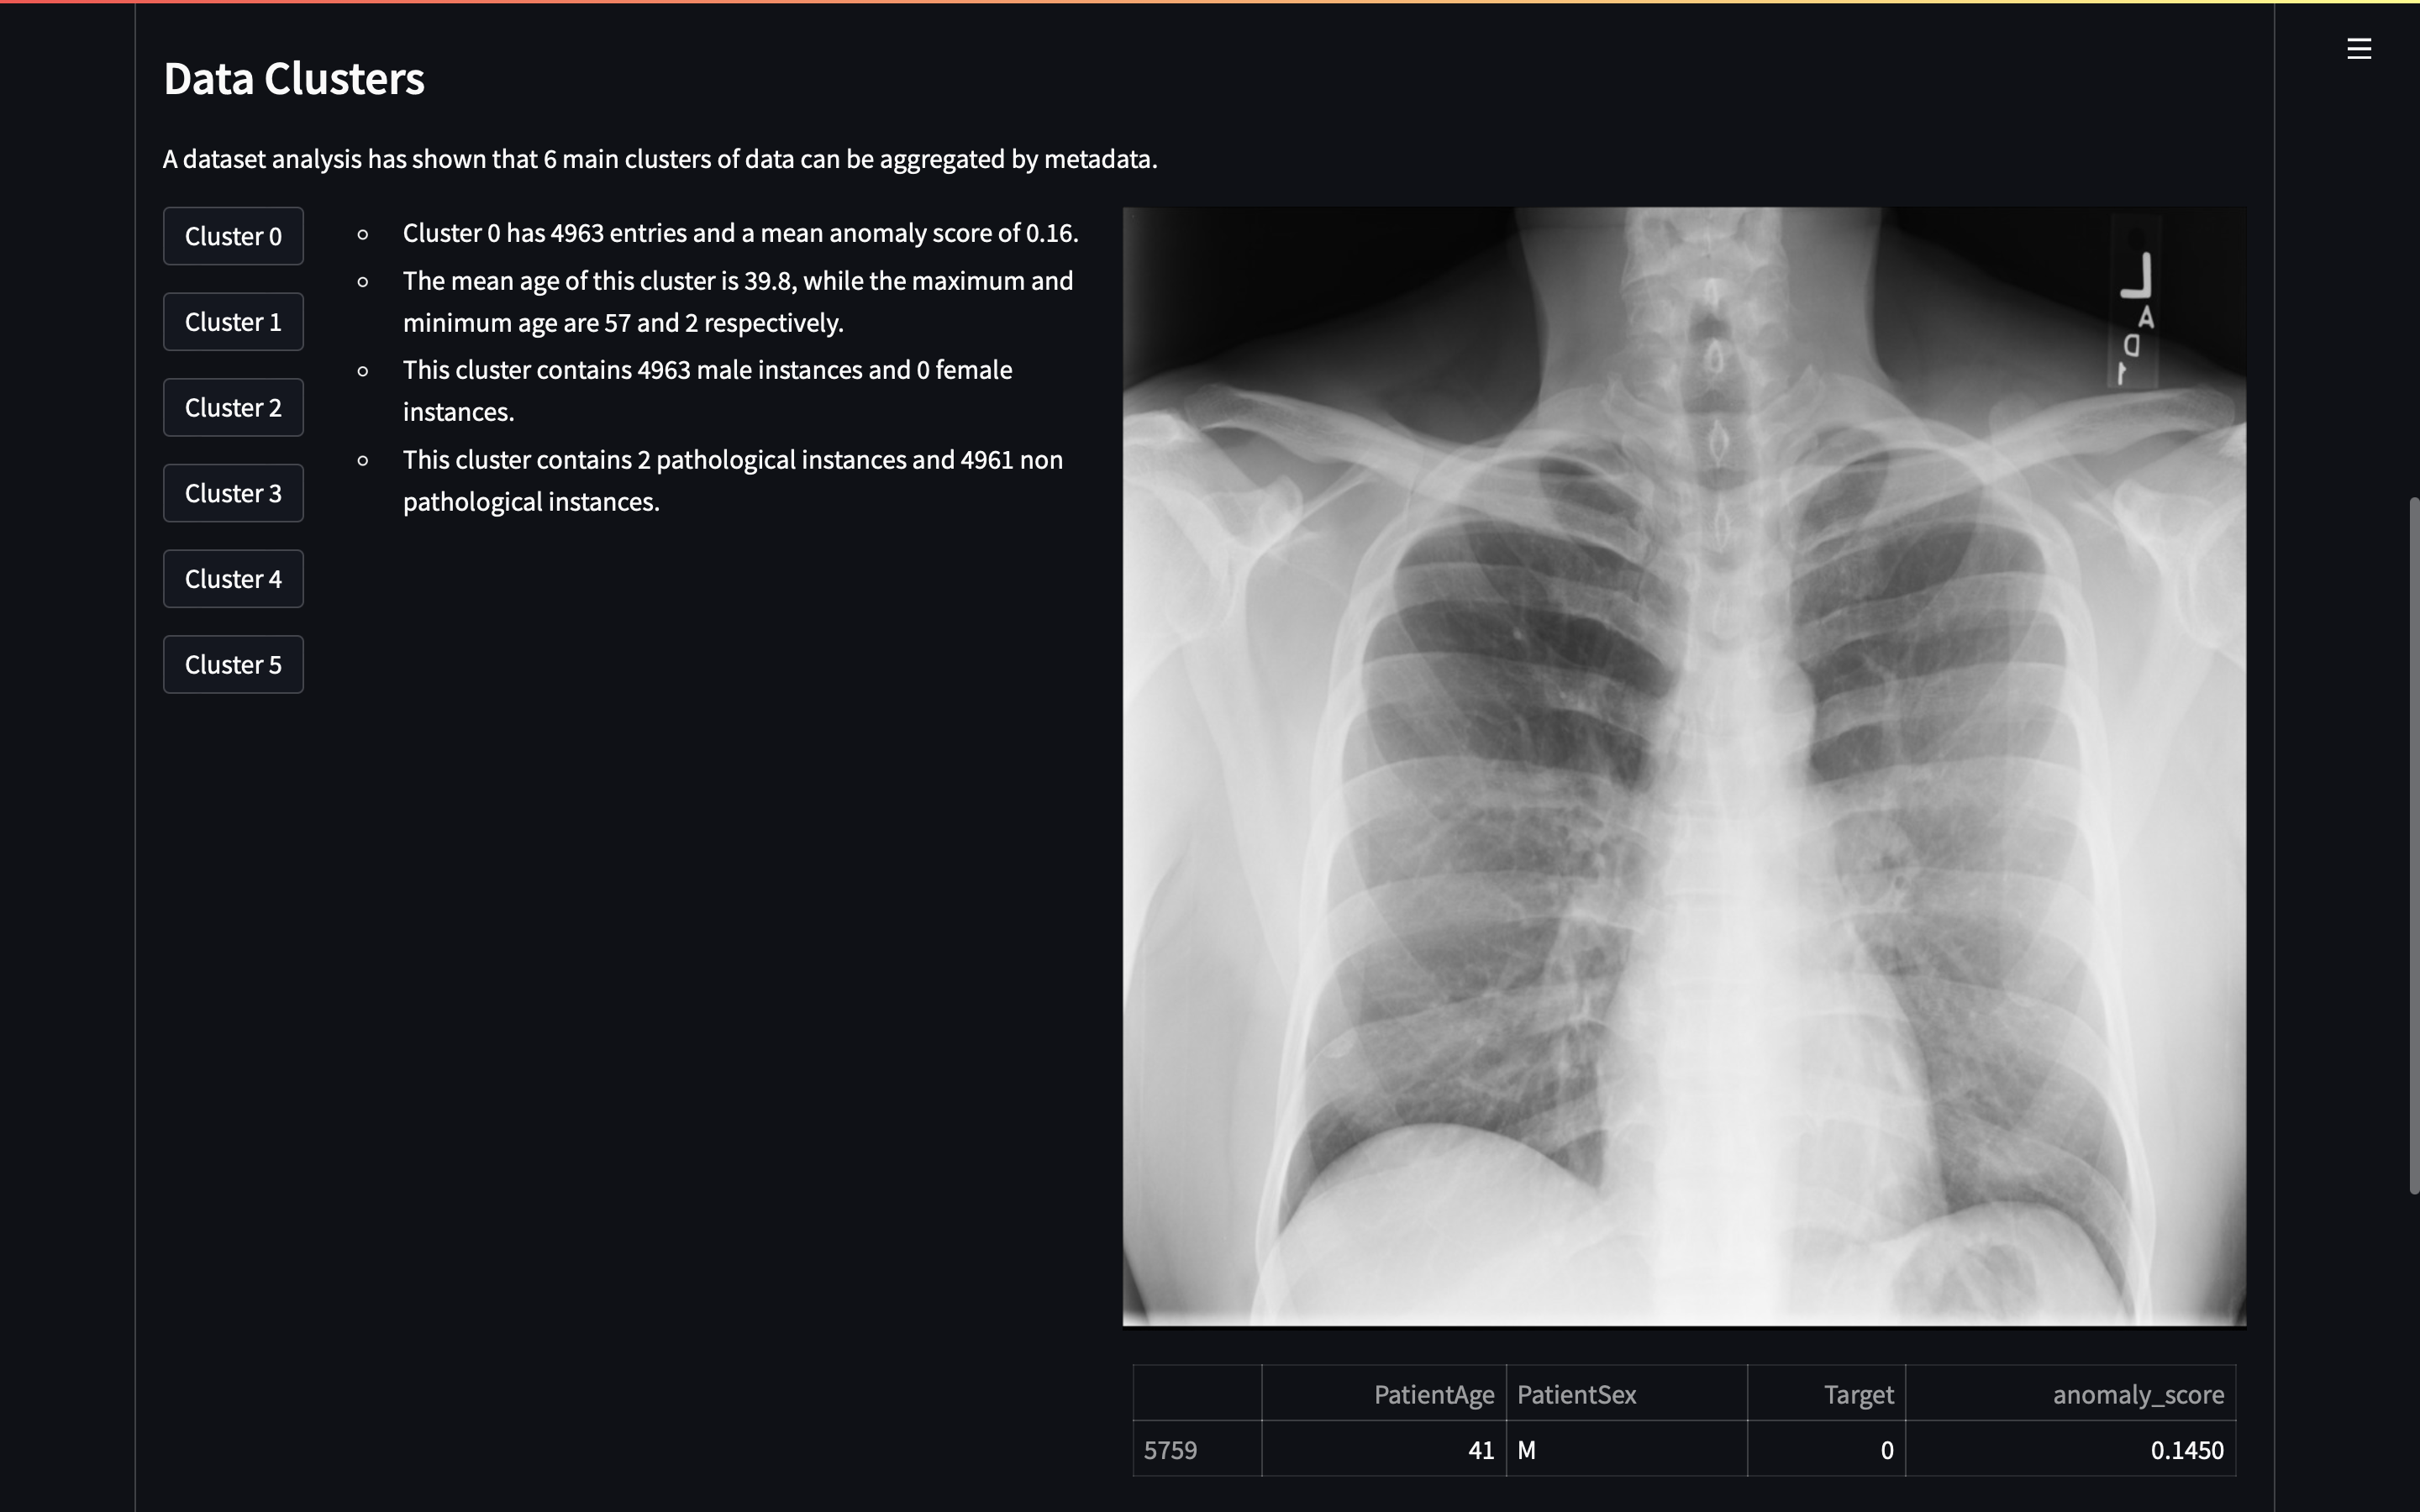
\includegraphics[width=\textwidth]{img/screenshots/samples/large/l_data_clusters.png}
    \caption{Dialogue Sample - Data Clustering Functionality (large display)}
    \label{fig:samples_l_data_cluster}
\end{figure}

\begin{figure}[htbp]
    \centering
    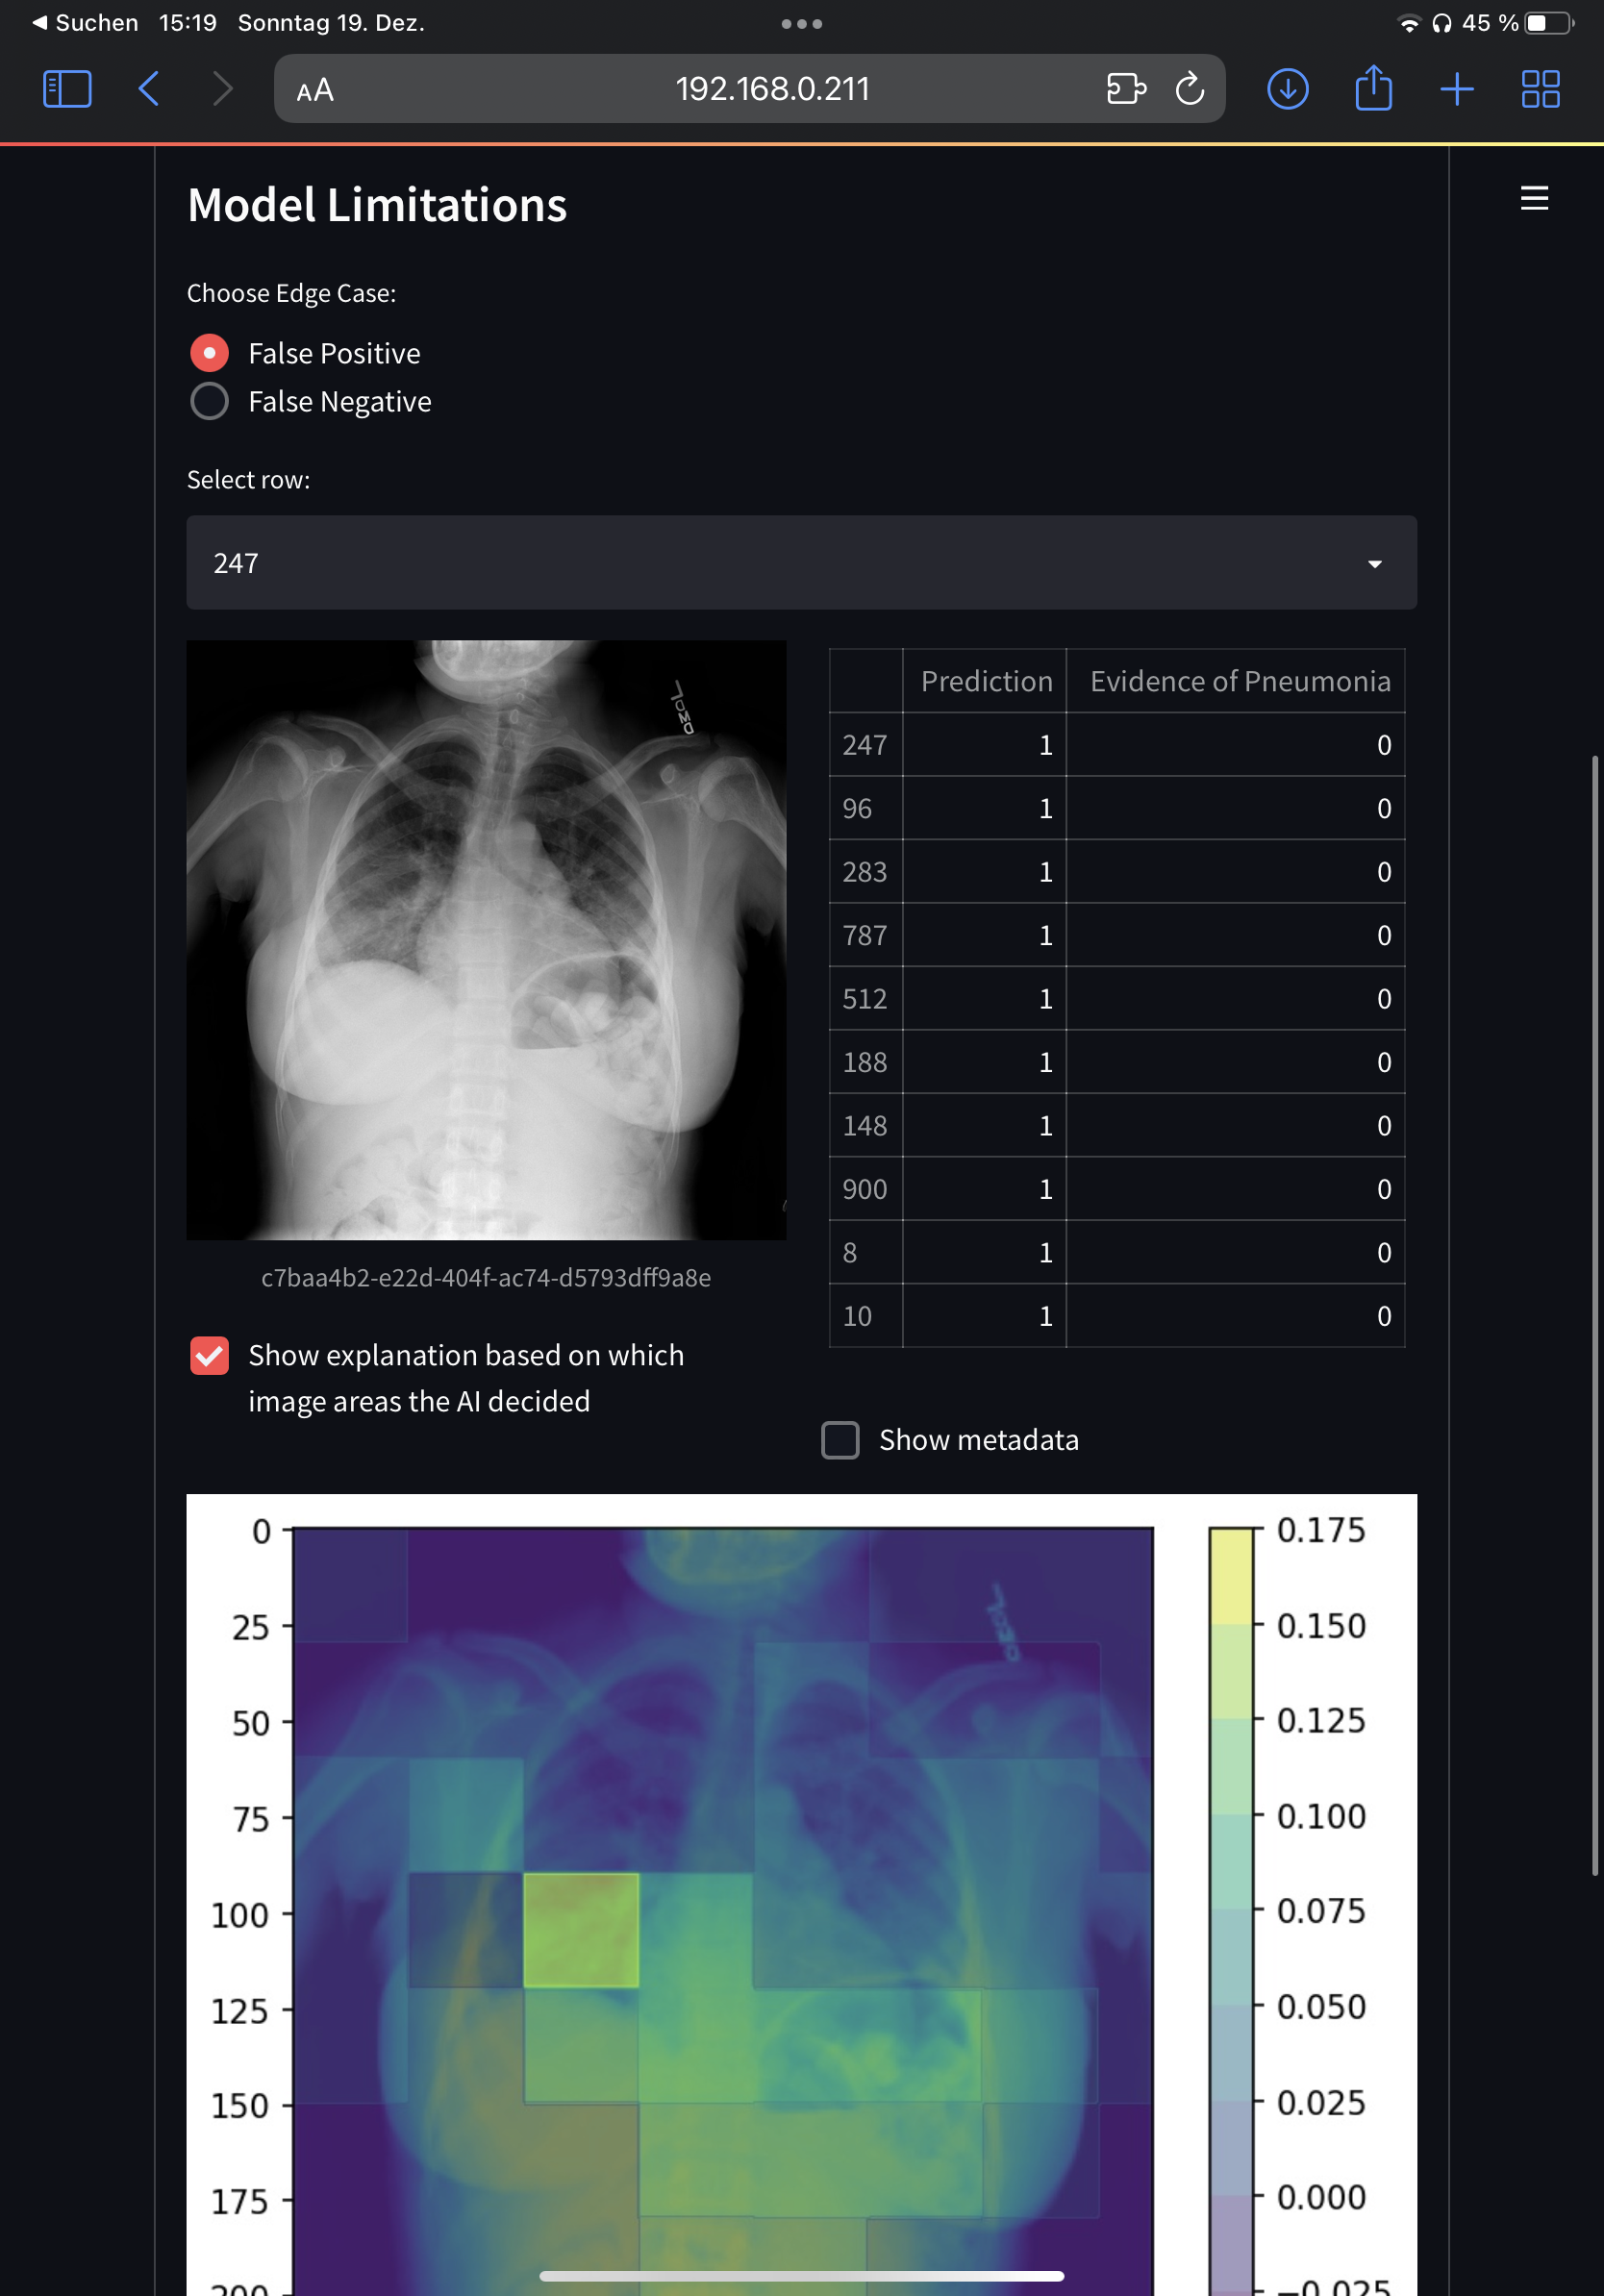
\includegraphics[width=\textwidth]{img/screenshots/samples/medium/m_limits.PNG}
    \caption{Dialogue Sample - Data Clustering Functionality (medium display)}
    \label{fig:samples_m_limits}
\end{figure}

\begin{figure}[htbp]
    \centering
    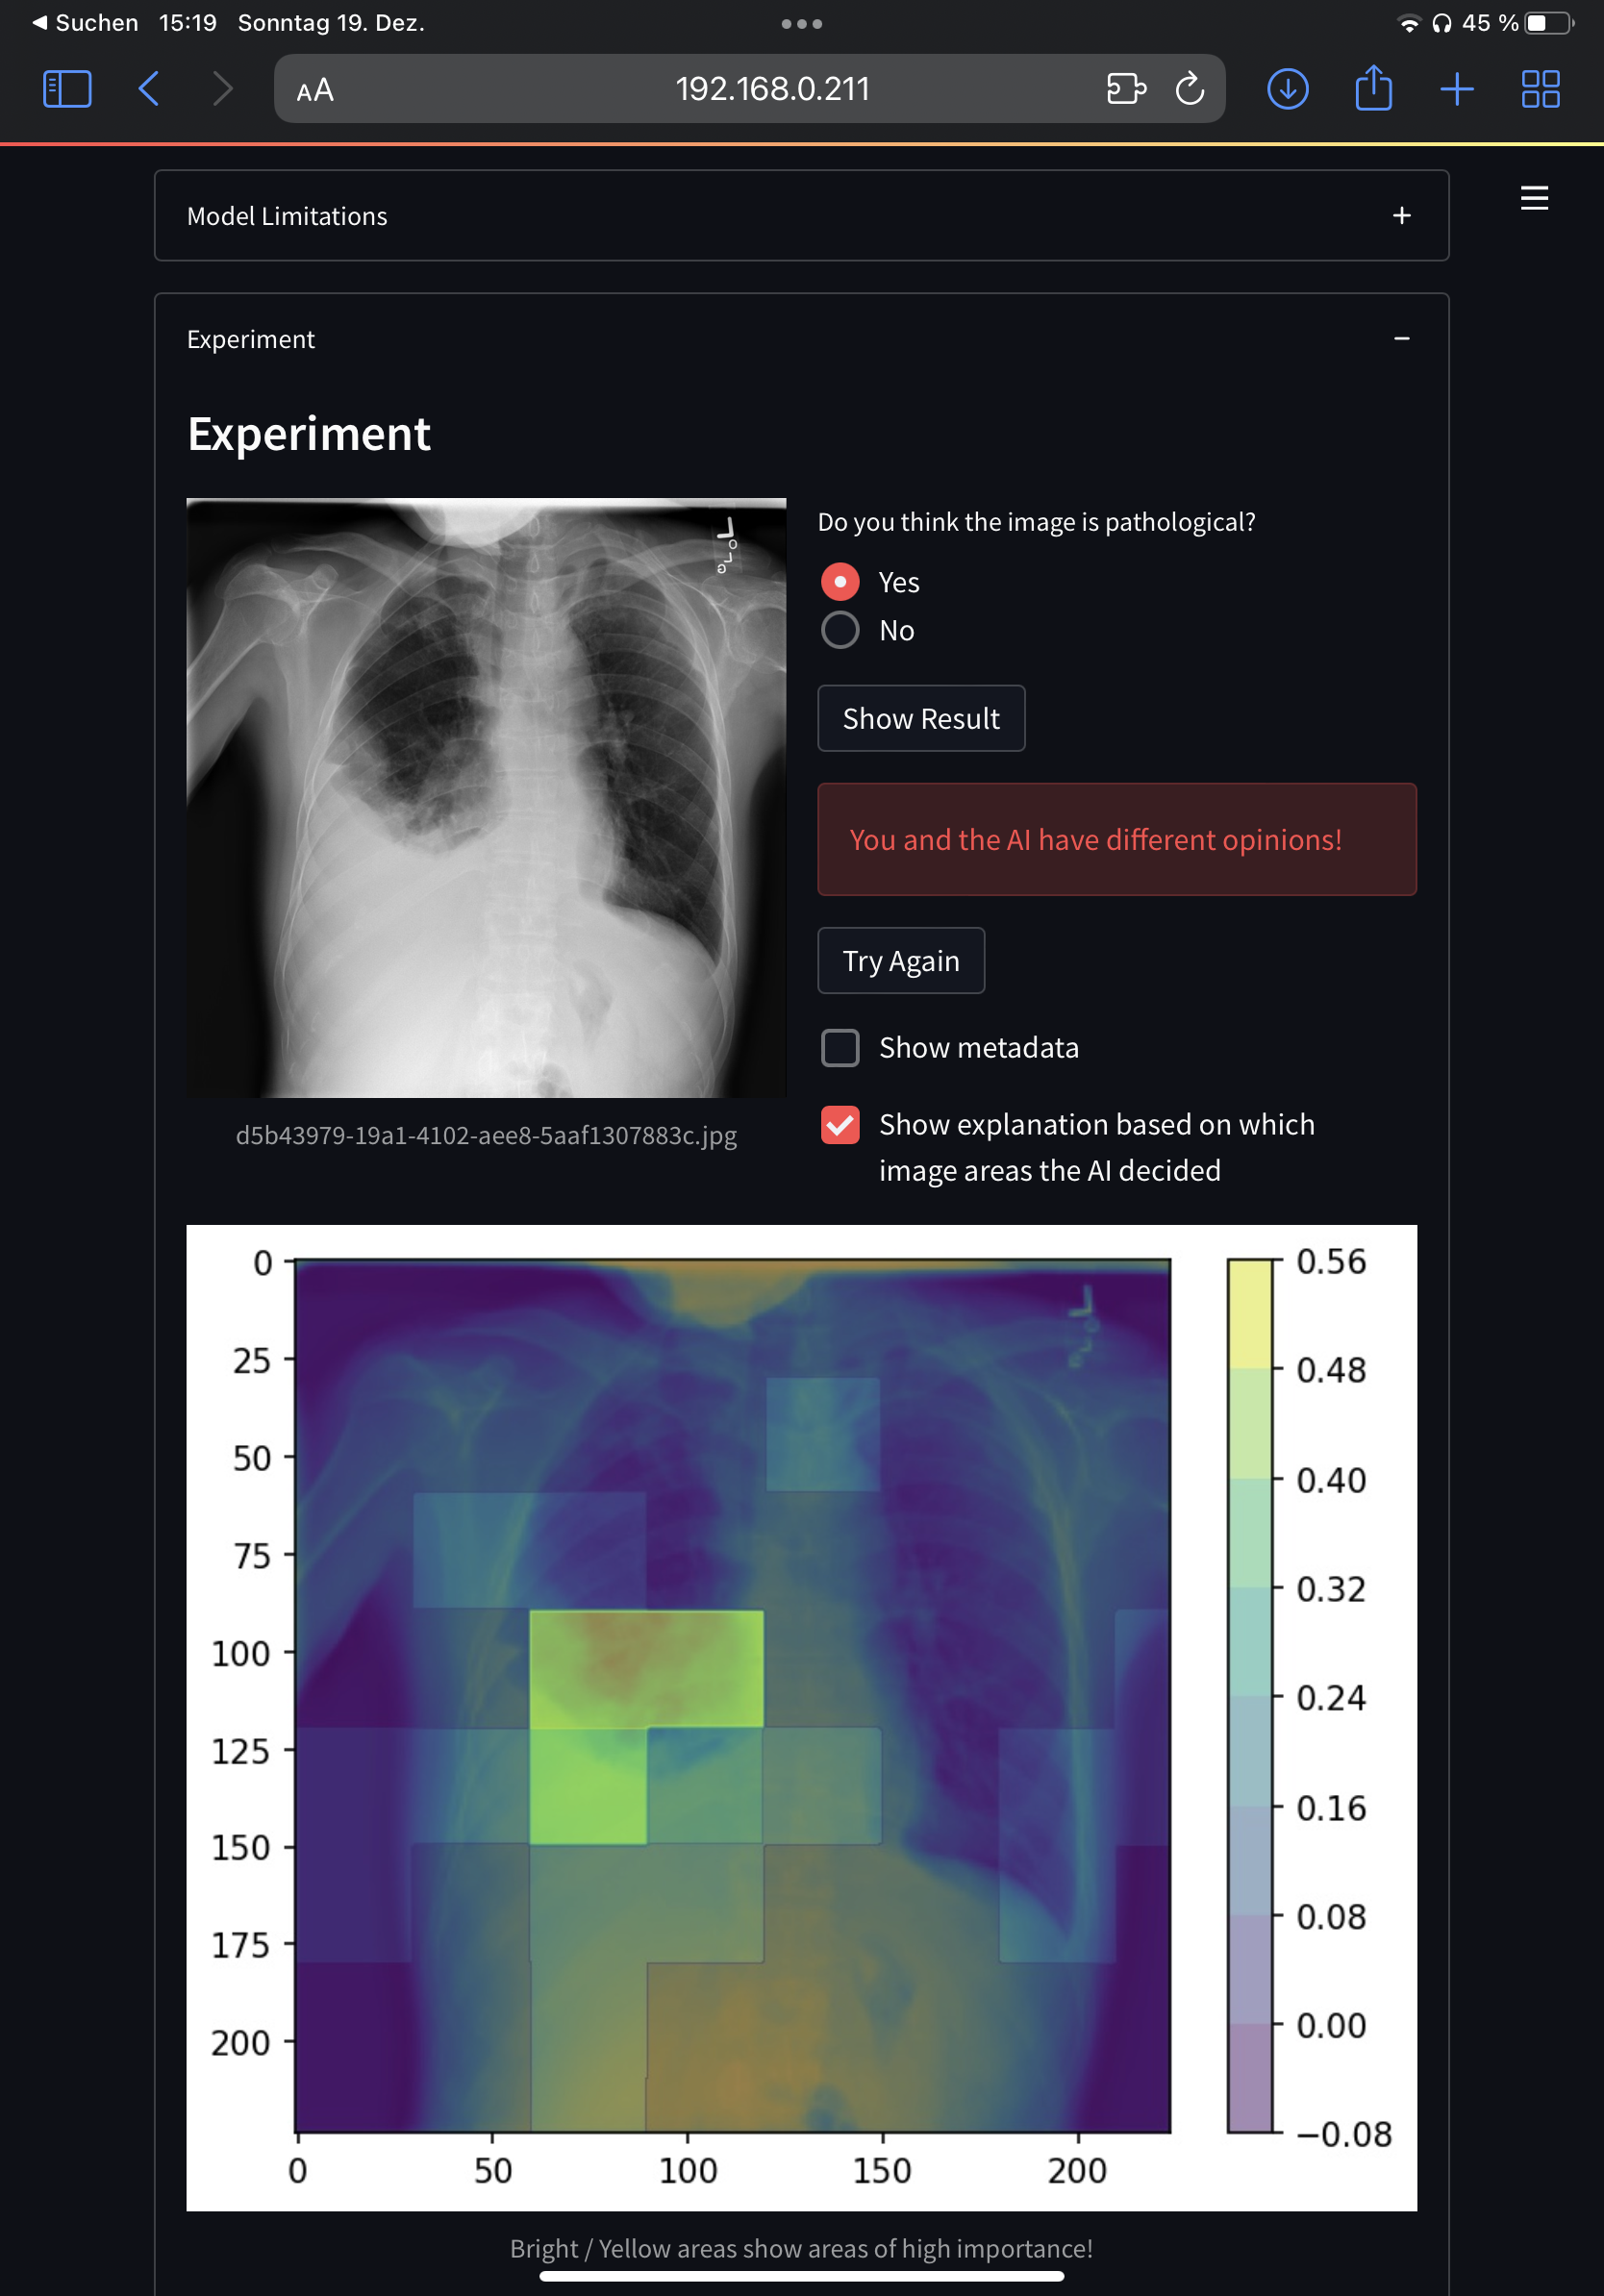
\includegraphics[width=\textwidth]{img/screenshots/samples/medium/m_occlusion.PNG}
    \caption{Dialogue Sample - Experiment Functionality (medium display)}
    \label{fig:samples_m_experiment}
\end{figure}

\begin{figure}
    \centering
    \subfigure[]{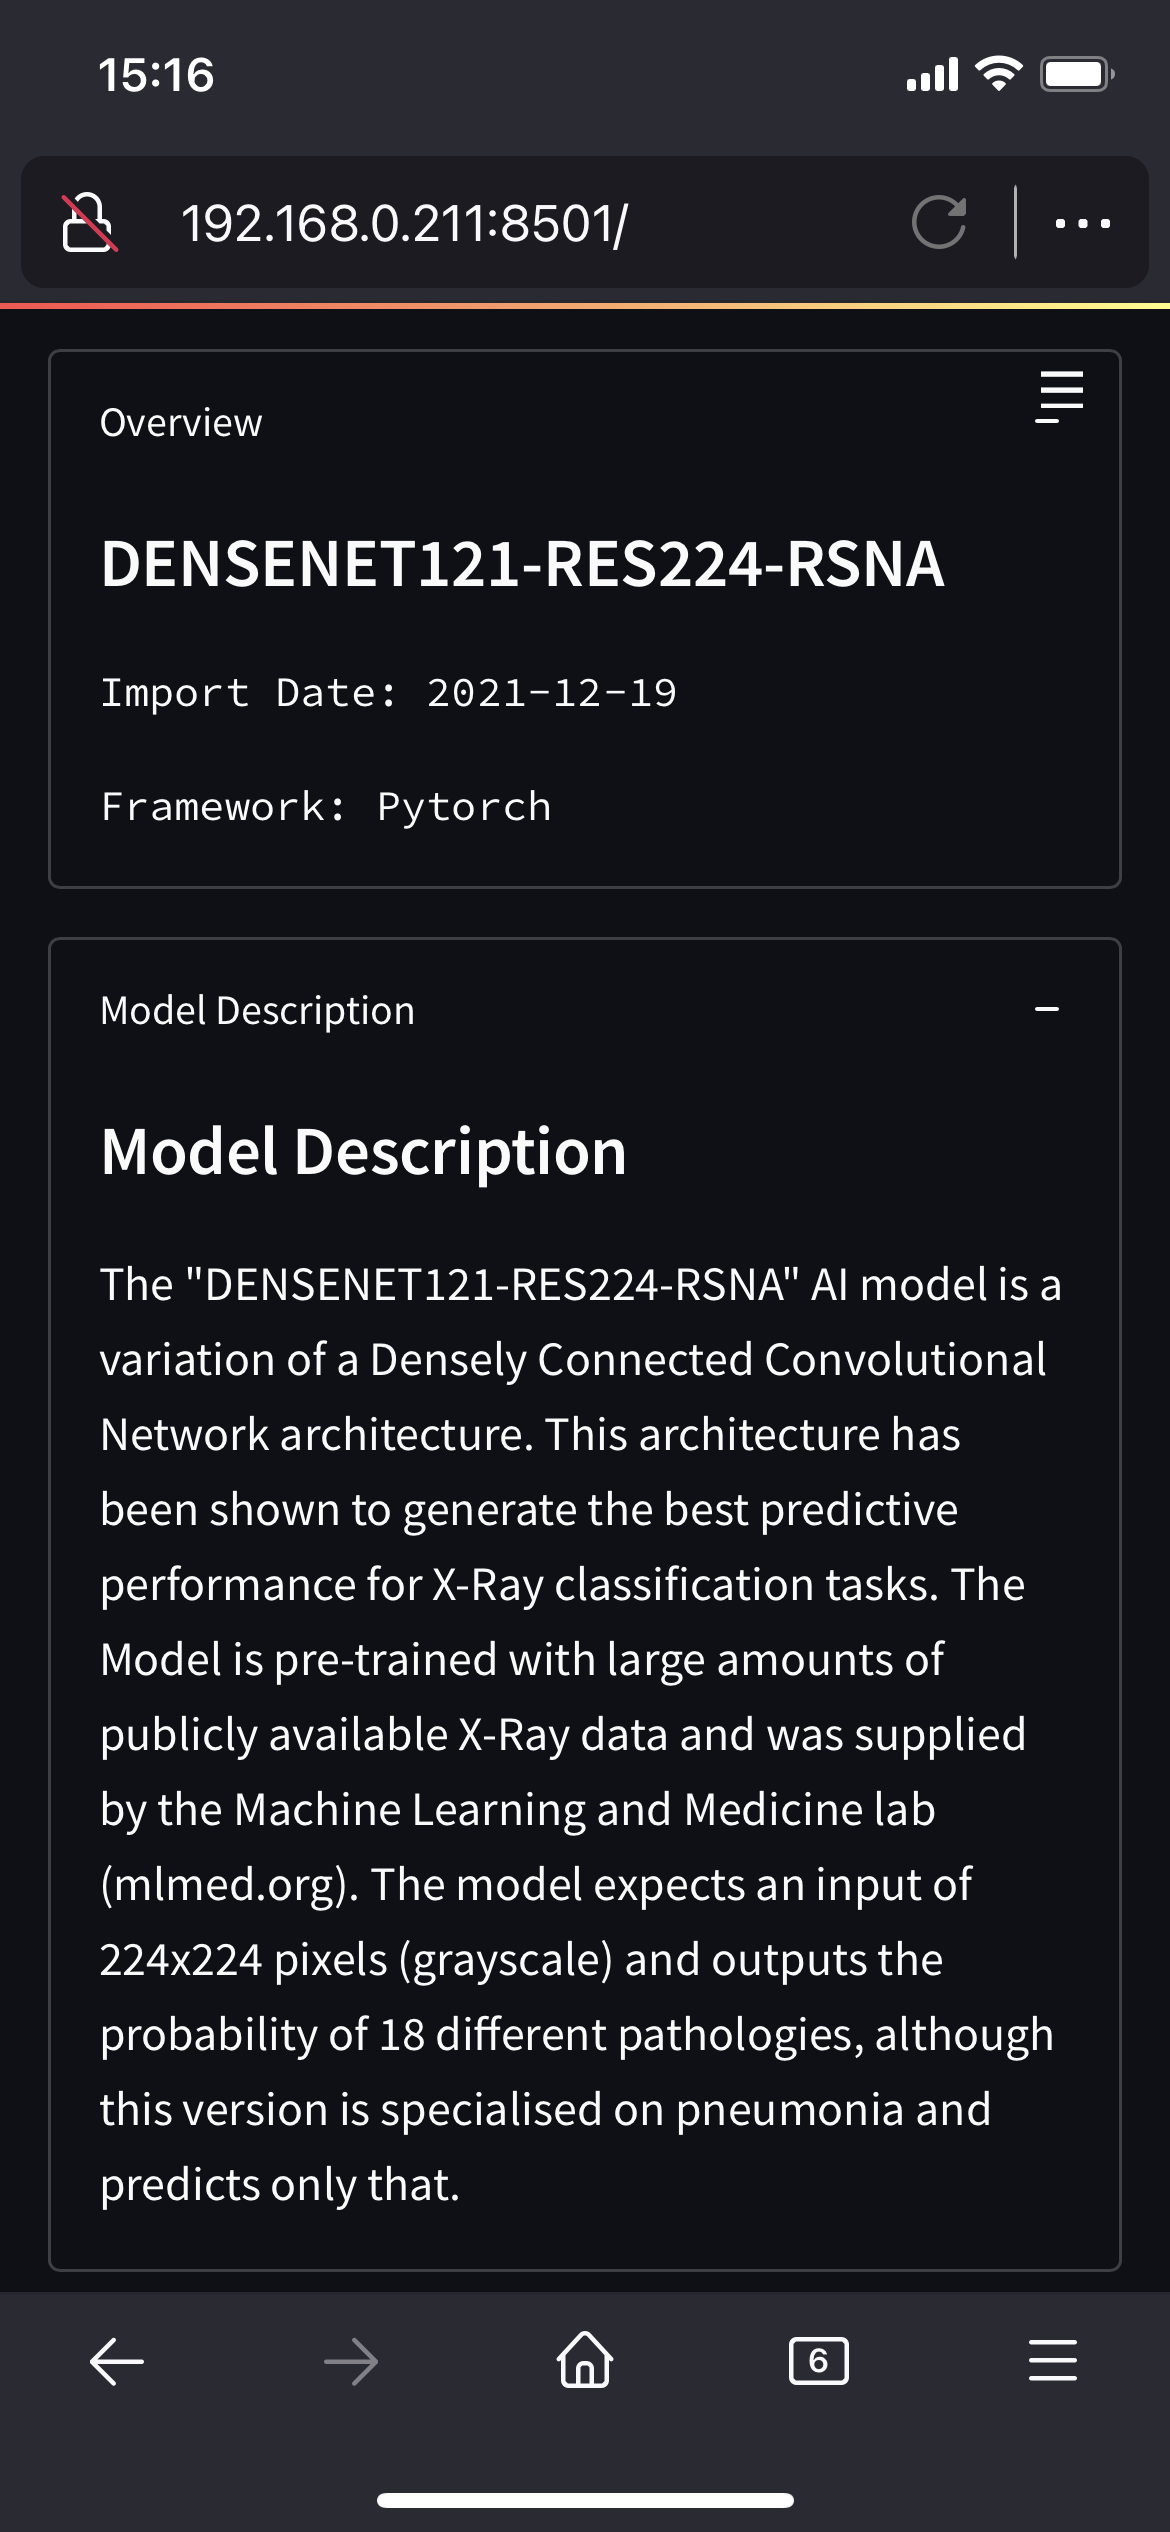
\includegraphics[width=0.4\textwidth]{img/screenshots/samples/small/s_overview.PNG}} 
    \subfigure[]{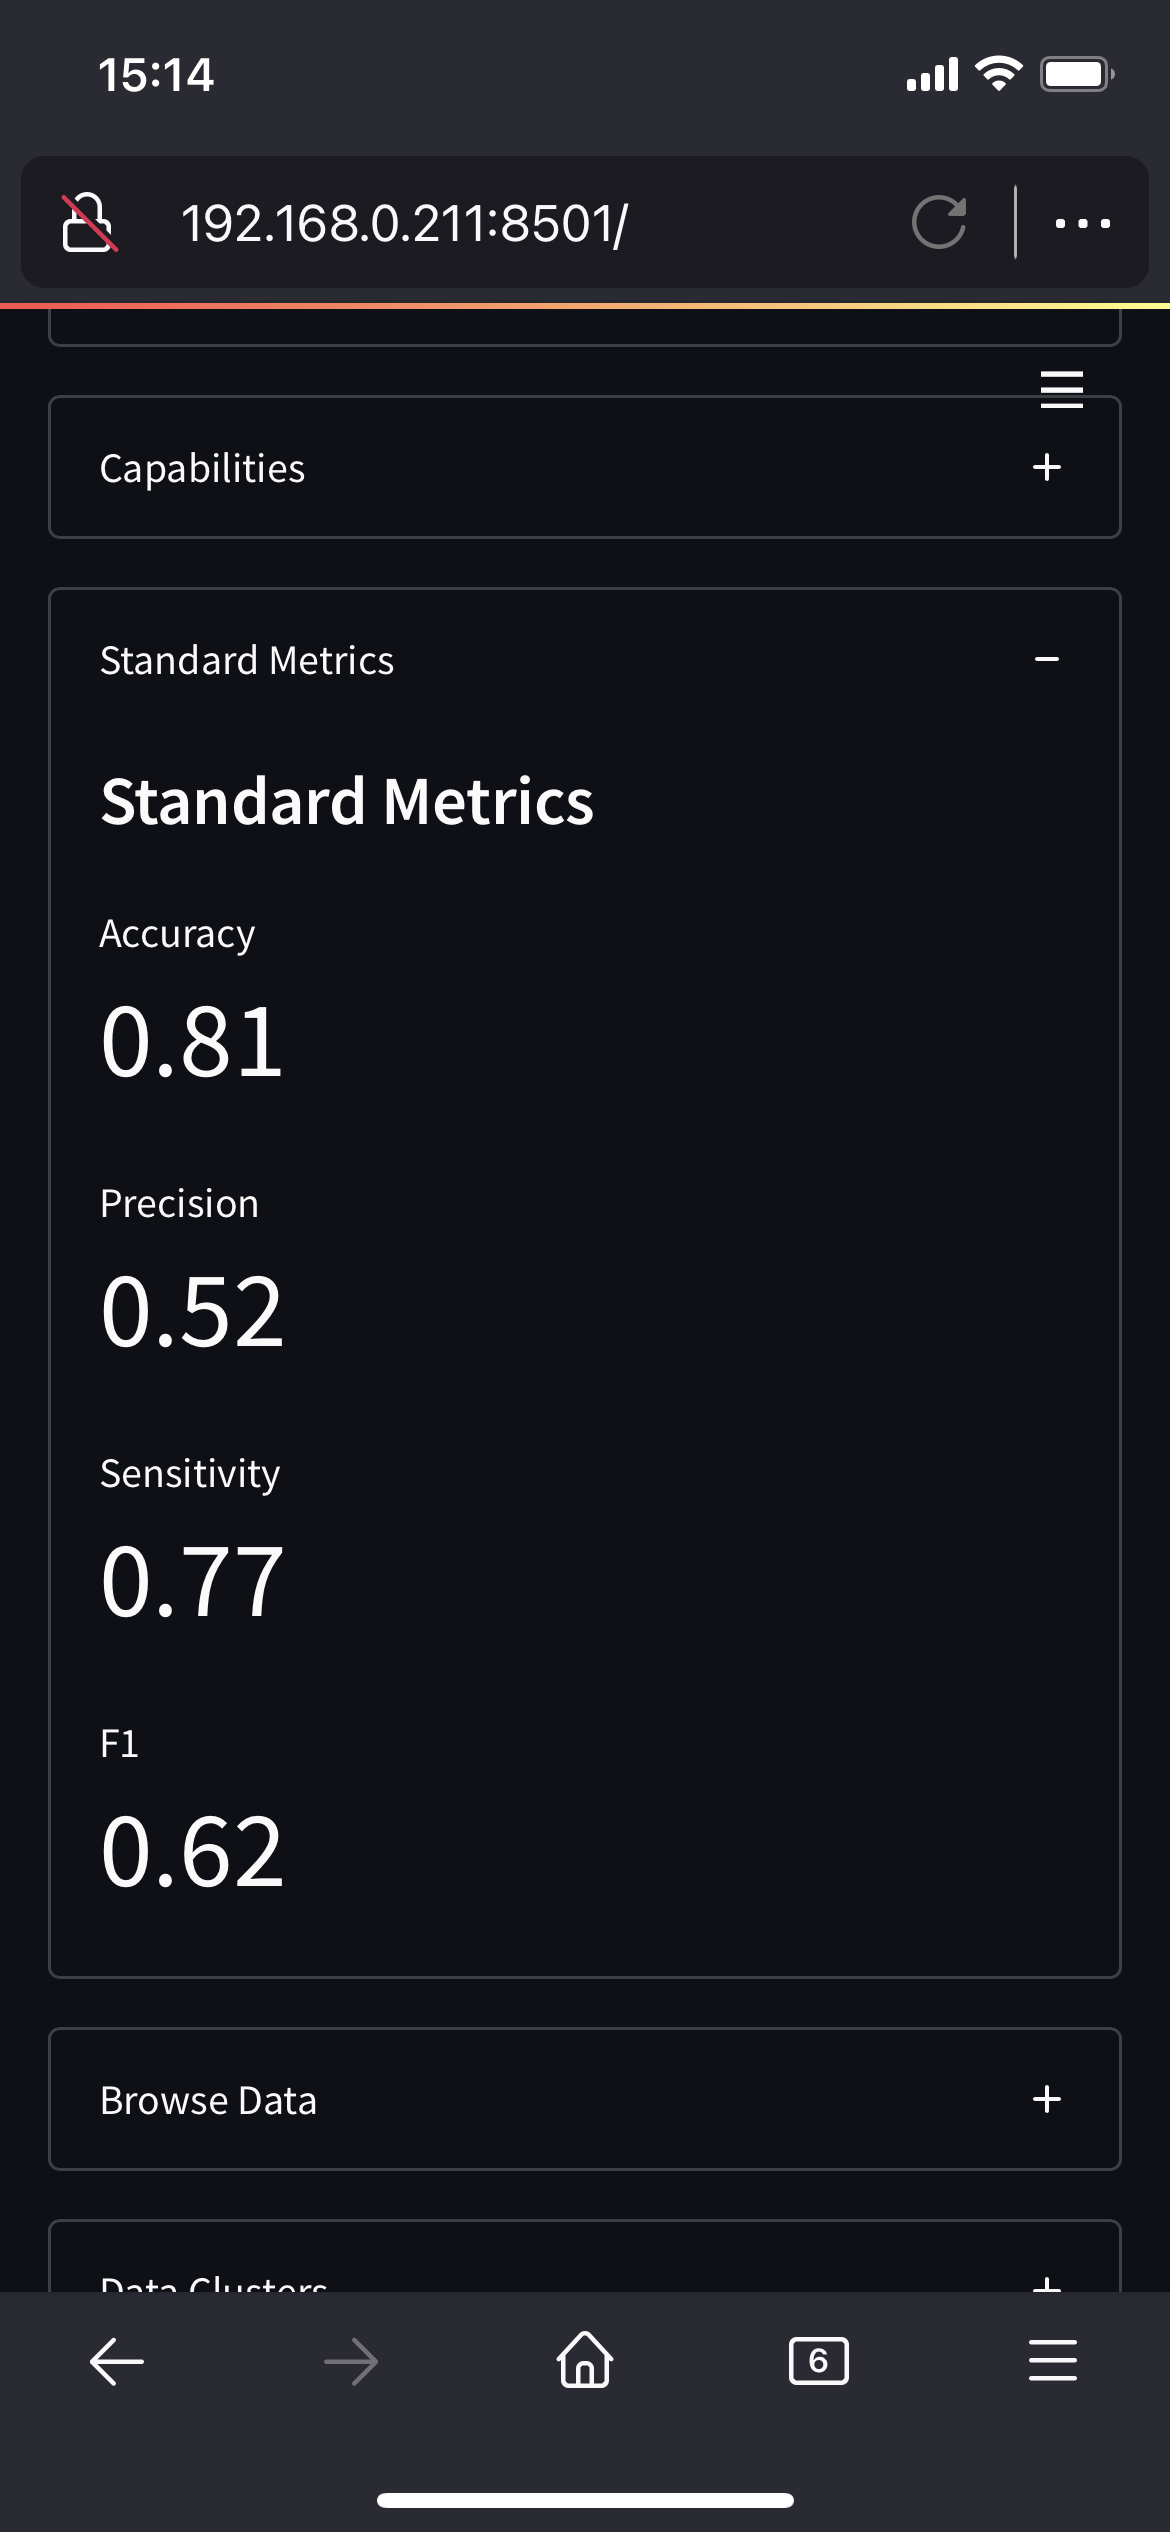
\includegraphics[width=0.4\textwidth]{img/screenshots/samples/small/s_metrics.PNG}} 
    \caption{(a) Overview Functionality (small display) (b) Metrics Functionality (small display)}
    \label{fig:samples_s_overview_metrics}
\end{figure}

\begin{figure}
    \centering
    \subfigure[]{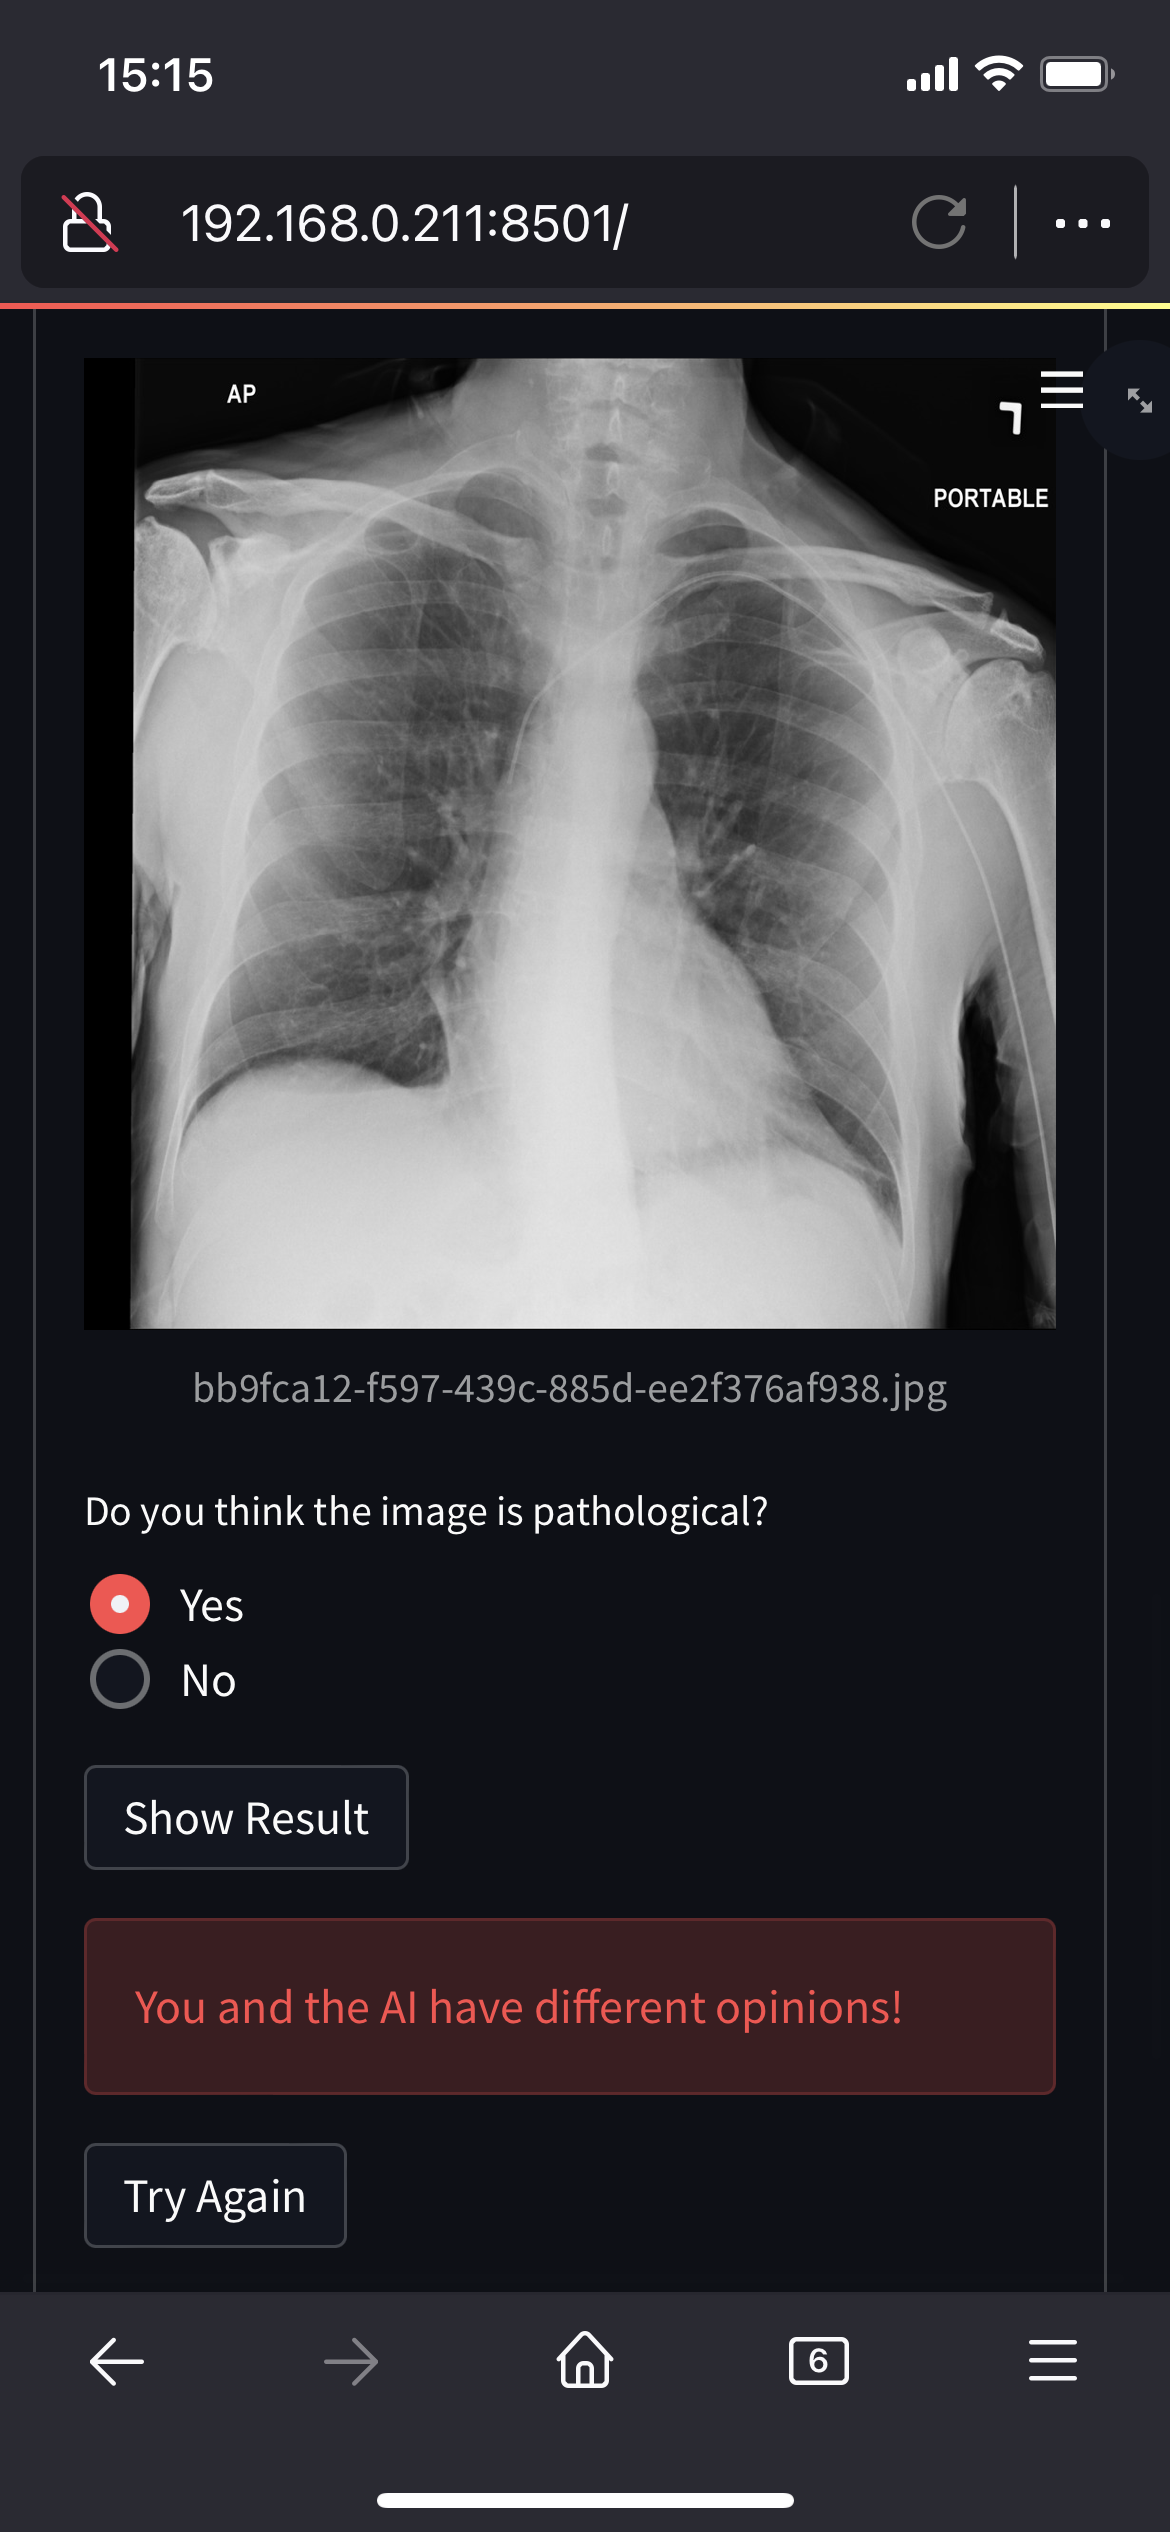
\includegraphics[width=0.4\textwidth]{img/screenshots/samples/small/s_experiment.PNG}} 
    \subfigure[]{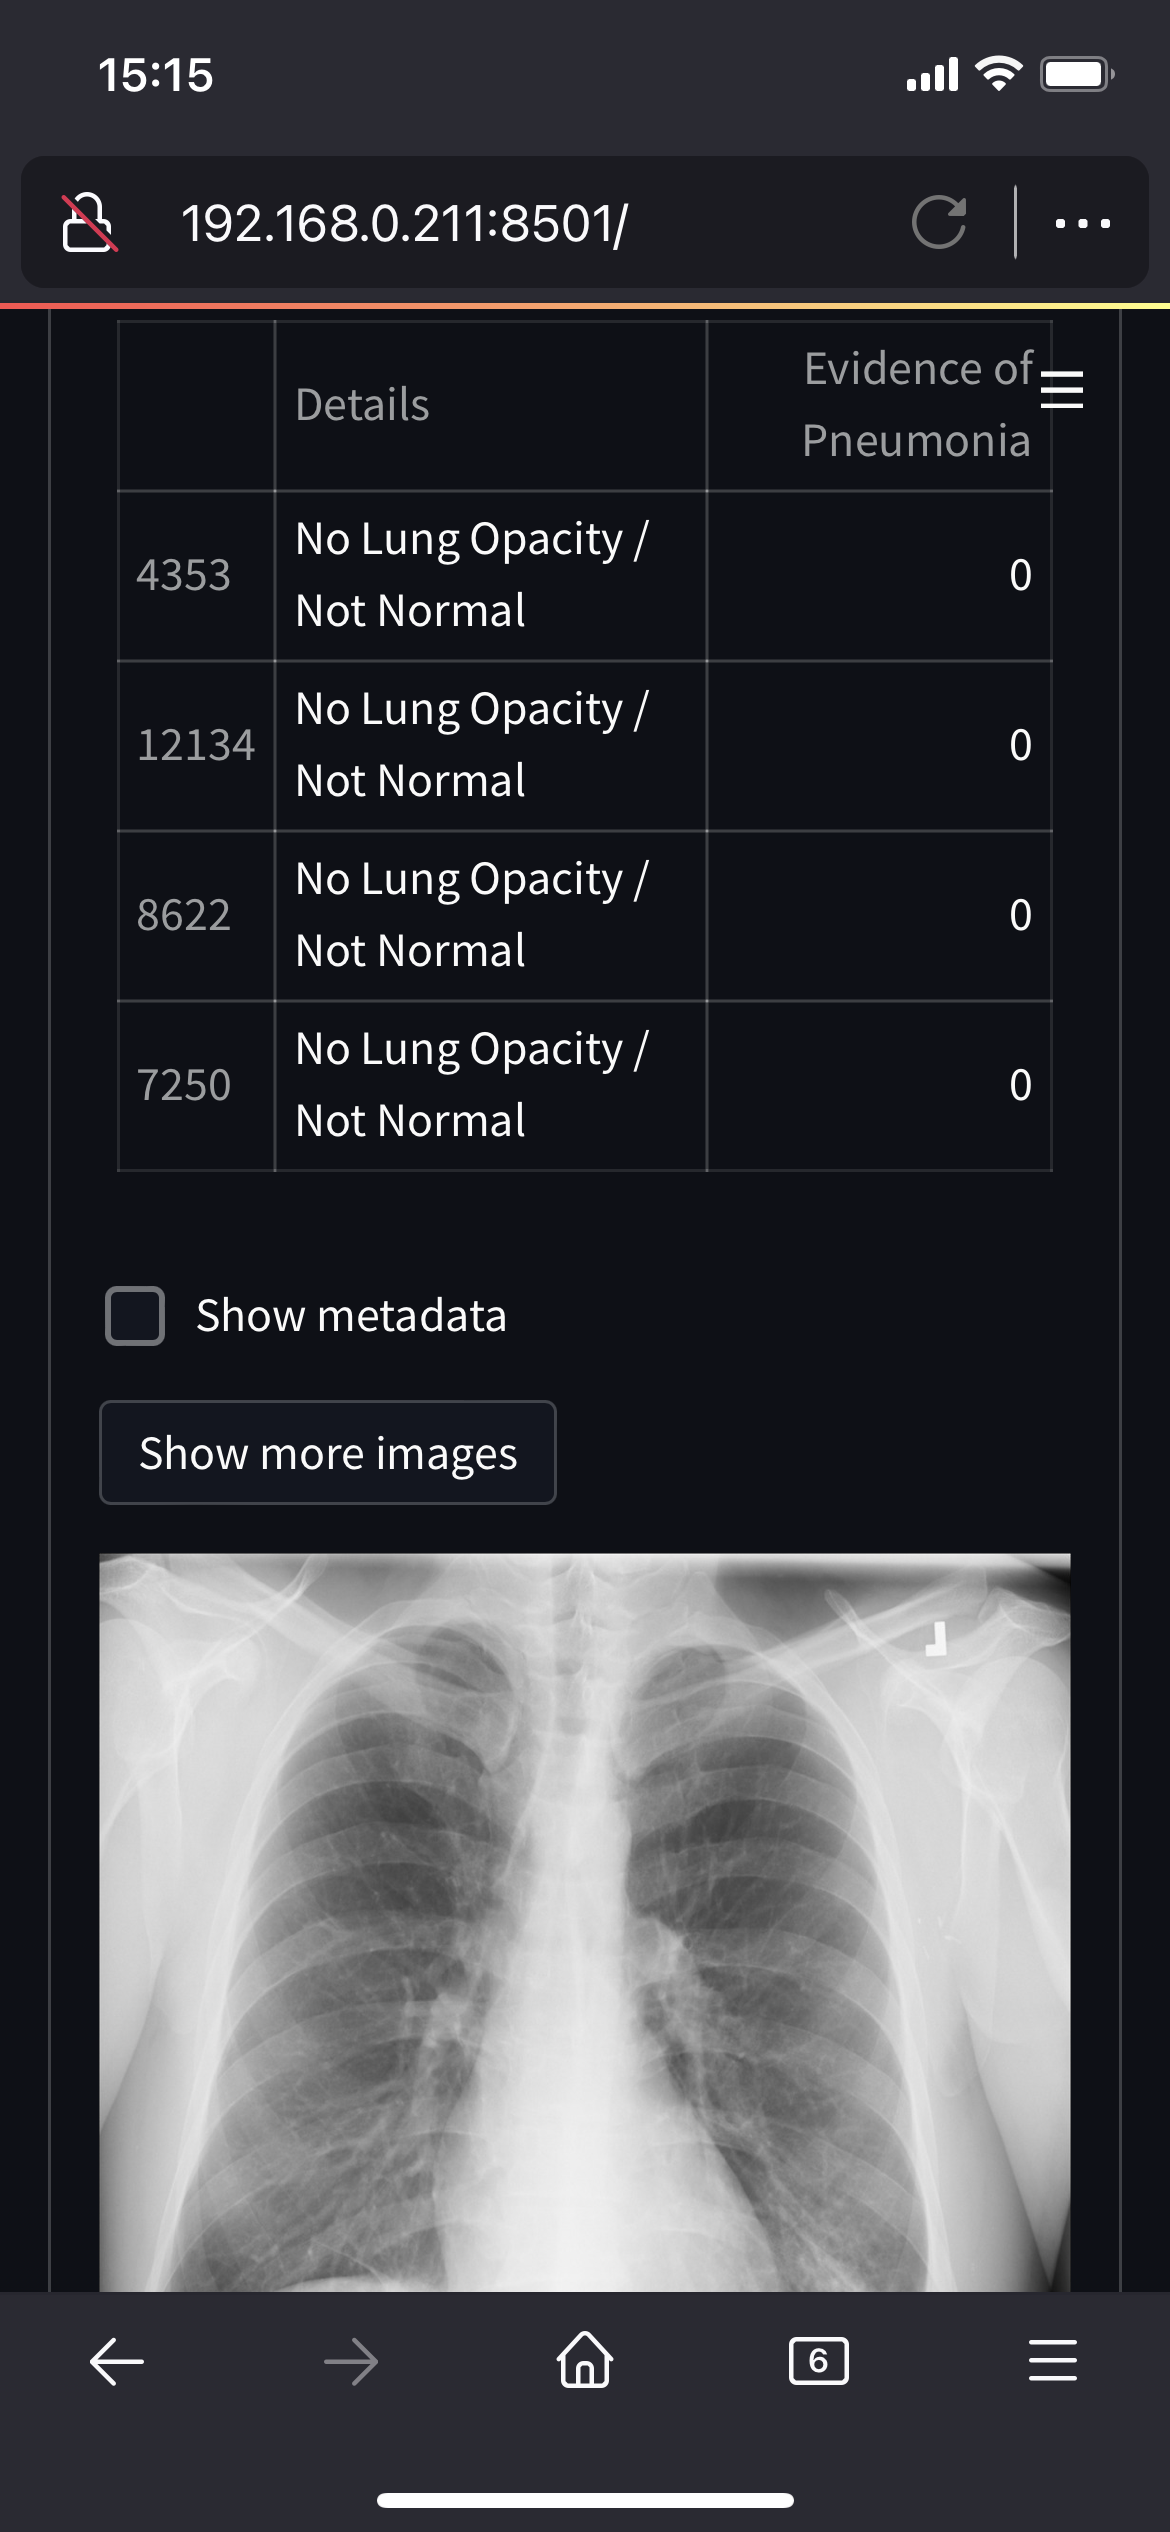
\includegraphics[width=0.4\textwidth]{img/screenshots/samples/small/s_browse.PNG}} 
    \caption{(a) Experiment Functionality (small display) (b) Browse Functionality (small display)}
    \label{fig:samples_s_experiment_browse}
\end{figure}

\newpage
\chapter{Summative Evaluation}\label{chapter:evaluation}
Following the principles of a human centered development of software, a summative evaluation of the AI assessment prototype was conducted. This is important to assess the efficiency, effectivity and quality of the solutions from conception to implementation \parencite{gediga_evaluation_2002}. The following sections will give insights into the concrete goal, the used methods, the study design and the results of the evaluation.

\section{Goal}
In the context of the thesis it is important to study the concrete effects of the AI assessment system prototype on the user regarding information processing, trust and workload. These three aspects are directly derived from the research questions and the goals of the thesis (see \autoref{section:goals}). Assessing explainability and trustworthiness of AI models through the usage of an assessment system and evaluation with potential users of such system is the main goal. The focus is on the effects of the interactive explanation methods described in \autoref{subsection:explanation_techniques}. The study also aims to generate insights into the differences of the guided versus unguided interaction modes. The results of the evaluation will create a foundation for further discussion and research on this topic, especially regarding the human factors in the interaction of humans and computers respectively intelligent system, such as AI models.

\section{Methods}
To gain insights on the effects of the AI assessment system on the potential users a on-site experiment was conducted. The study was realized in German, because the place of evaluation was the university of Lübeck, where most participants are only fluid in the German language. To assess the effects of the AI assessment system and the different interaction modes (guided versus unguided) a mixed study including within-subject and between-subject aspects was developed aiming at approximately 30 subjects. The effects of the independent variables (interaction with the AI assessment system and guided versus unguided interaction) on the dependent variables (Subjective Information Processing Awareness (\textbf{SIPA}), Trust and Workload) were studied.

It is important to mention the focus on subjective measures in this study, as the main aspects of trustworthiness and explainability of AI models are also highly subjective. Therefore mainly subjective data was collected - with the exception of one objective workload measure. The complete evaluation questionnaire can be found in \nameref{appendix:evaluation_questionnaire}.

\subsection{Participants}
The participants of the evaluation were chosen to be medical students, as this is largely in line with the main user group described in \autoref{section:user_analysis}. Although medical professionals such as interviewed in \autoref{subsection:interviews} are preferable but are particularly difficult to make appointments with. Since the study aimed to evaluate approximately 30 participants in a short time, a high turn around count was important. To further increase the initiative of participating in the study a raffle was set up, drawing four winners rewarded with 50€ each.

The study was announced on multiple channels (university internal platform and research partner contacts) two weeks before the three week long execution period. In total, \textit{N} = 14 people participated in the study. All participants were medical students from the university of Lübeck with an age ranging from 21 to 32, 6 of which were male and 8 female. The lowest semester recorded was 5th and the highest was 11th. All participants stated having at least a fundamental knowledge in radiology, but have a very mixed level of affinity for technology interaction. \autoref{table:evaluation_participants} compiles the information of the 14 participants.

\begin{table}[htbp]
    \centering
    \begin{tabularx}{0.45\textwidth}{ l c c c }
        \toprule
        & age & semester & ATI score \\
        \midrule
        \textit{N} & 14 & 14 & 14 \\
        \textit{M} & 24.36 & 8.07 & 3.91 \\
        \textit{SD} & 3.34 & 2.36 & 0.83 \\
        \textit{Min} & 21 & 5 & 2.11 \\
        \textit{Max} & 32 & 11 & 5.33 \\
        \bottomrule
    \end{tabularx}
    \caption{Descriptive Statistics of Basic Information on the Evaluation Participants}
    \label{table:evaluation_participants}
\end{table}

\subsection{Design}
The study was designed to incorporate within-subject and between-subject components in an one-to-one on-site experiment. The within-subject component is the interaction with the system, since all subjects interacted with the assessment system. The between-subject component is the interaction style (guided versus unguided), as the participants were split into two groups of the same size, one interacting with the guided version while the other interacting with the unguided version. \autoref{fig:Study_design} showcases the study design with the subject components and the data acquisition points: Firstly, the by e-mail recruited participants were introduced to the context and content of the study. After consenting to a data protection agreement, the participants completed the first questionnaires, which act as the foundation for comparing the information processing and trust before and after the interaction. During the interaction with the system, the time spend on the interaction was measured as a indication of objective workload (with a cut off at 15 minutes). After the interaction the participants completed the last questionnaires. This design allows for comparison of various subjective characteristics before and after the assessment system interaction while also measuring differences between the interaction styles in an overall duration of approximately 30 minutes.

\begin{figure}[htbp]
    \centering
    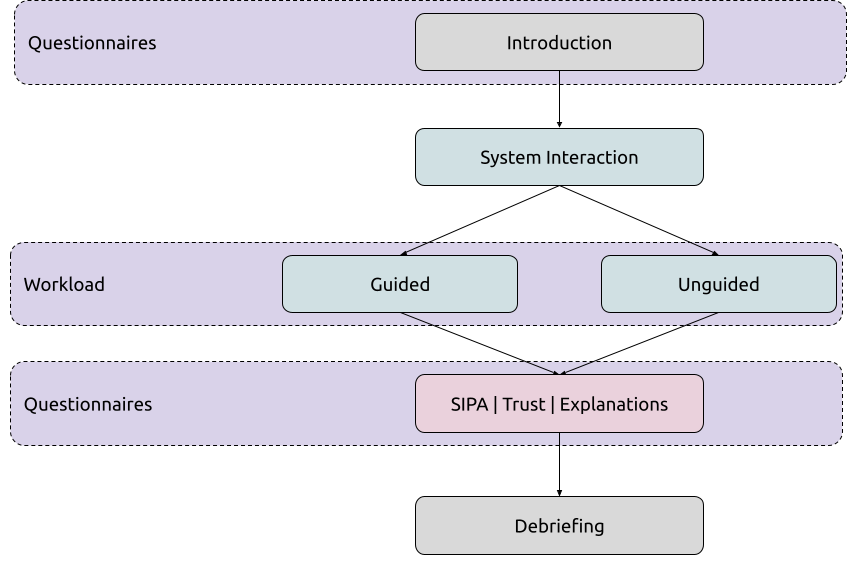
\includegraphics[width=0.9\textwidth]{img/study_design.png}
    \caption{Study Design}
    \label{fig:Study_design}
\end{figure}

\subsection{Setting and Instruments}
\paragraph{Setting}\mbox{} \\
The experiment was conducted on site at the university of Lübeck. For the timeframe of the evaluation the usability lab was provided by the Institute for Multimedia and Interactive Systems (IMIS), where the study was carried out. The lab was used for the completition of questionnaires and the interaction with the assessment system. The actual interaction was carried out on a 2016 MacBook Pro (i5, 16GB RAM, MacOS 12.0.1, 13"), where the whole application was running (backend and frontend). The web browser used for displaying the GUI was Safari (version 15.1). Only one participant at a time was evaluated, because special requirements in the form of a hygiene concept had to be met due to the ongoing pandemic situation.

\paragraph{Application usage}\mbox{} \\
The participants were presented with the application as implemented in \autoref{chapter:implementation} - either with the guided or the unguided version (see \autoref{chapter:dialogue_samples}). Additionally it was made sure, that the participants could use the peripherals to interact with the GUI in the Safari browser. After the initial introduction, the participants were told to freely interact with the application for a maximum of 15 minutes.

\paragraph{Questionnaires}\mbox{} \\
The study included questionnaires to be answered before and after the interaction with the system. The questionnaires used in this study were:
\begin{itemize}
    \item Basic Demographic Query (pre)
    \item Subjective Information Processing Awareness Scale (SIPA) \parencite{schrills_sipas_2021} (pre \& post)
    \item Facets of System Trustworthiness (\textbf{FOST}) \parencite{franke_advancing_2015} (pre \& post)
    \item Affinity for Technology Interaction (ATI) \parencite{franke_personal_2019} (pre)
    \item Explanation Satisfaction Scale (\textbf{ESS}) \parencite{hoffman_metrics_2019} (post)
    \item NASA Task Load Index (\textbf{NASA-TLX}) \parencite{hart_nasa-task_2006} (post)
\end{itemize}
The whole compiled questionnaire with all sub questionnaires and explanatory texts in German can be found in \nameref{appendix:evaluation_questionnaire}. The questionnaire results were digitalized and aggregated in an excel sheet to include all answers per participant (each participant got a row in the sheet identified by a pseudonym). Per participant the results  of each sub-questionnaire were evaluated by calculating the mean with regards to inverted items, as described by the original authors \parencite{schrills_sipas_2021,franke_personal_2019,franke_advancing_2015,hoffman_metrics_2019,hart_nasa-task_2006}. Each resulting mean value was appended in its own column.

\subsection{Procedure}\label{subsection:procedure}
The participants were invited individually to the study in the usability lab of the university of Lübeck. Firstly the participants were greeted and the necessary covid-19 measures were taken - only vaccinated, recovered or tested people could participate under strict hygienic requirements. After the greeting, the briefing started. The briefing included a spoken and written thematic introduction and a brief overview of the procedure. Additionally the participants got to read an explanation of the AI model used, the standard metrics and the assessment system. When the briefing was completed without open questions, the participants needed to consent to a data privacy agreement. This marks the start of the data acquisition, which takes place on paper (printed version of \nameref{appendix:evaluation_questionnaire}). The first half of the questionnaire included demographic, ATI, SIPA and FOST. SIPA and FOST here are referring to the explanation of the AI model in the briefing. After completing the first half, the interaction with the assessment system was started. The participants were asked to take place in front of the prepared laptop device with the instructions:

\begin{displayquote}
    "Your goal is to gather insights about the model's training data, strengths and limitations. Try to understand how the model is working through the interaction with the assessment system. For this you have 15 minutes. If you think that you will not be able to make any further discoveries before the 15 minutes are up, feel free to stop the interaction. If there are any questions or errors, feel free to ask for help."
\end{displayquote}

During the interaction the time was recorded. After the interaction the participants got to complete the second half of the questionnaire including SIPA, FOST, ESS and NASA-TLX. This marks the end of the data acquisition through the written questionnaire. After the competition, the debriefing started with the participants being asked whether there were things that went not so well, that struck them or created questions. Furthermore the participants were asked if they have comments on things that they liked about the interaction or general comments on the study. The data from the spoken debriefing was written down to complement the quantitative data.

\section{Results}\label{section:evaluation_results}
The descriptive statistics of the results are depicted in \autoref{table:evaluation_descriptive} and form the baseline for further analysis. These descriptive statistics can additionally be grouped up by the participant's interaction mode (guided vs. unguided), which is showcased in \autoref{fig:evaluation_descriptive_boxplots}, \autoref{table:evaluation_descriptive_guided} and \autoref{table:evaluation_descriptive_unguided}. When comparing the SIPA and FOST pre-test to the post-test scores, the statistics show that the interaction had effects on the explainability and trust. The objective time measured for the interaction was no indicator of the workload of the participants, as almost all used the full 15 minutes - for this the NASA-TLX score is more insightful as the unguided group has an overall higher task load index. Also the explanation satisfaction is overall higher in the unguided participant group.

To further evaluate the sampled data, a repeated measures analysis of variance (\textbf{ANOVA}) was conducted, in which the subjects are measured more than once to determine whether statistically significant change has occurred \parencite{vogt_dictionary_2011}. Because there are two independent variables (interaction \& guidance) a two-way ANOVA was applied to the data set from \autoref{table:evaluation_descriptive} for the dependent variables SIPA and trust (FOST). \autoref{table:anova_within_sipa}, \autoref{table:anova_between_sipa}, \autoref{table:anova_within_trust} and \autoref{table:anova_between_trust} showcase the results of the ANOVA. The results show a statistically significant change on the SIPA within-subject effect and the trust within-subject effect. However the between-subject effects do not display a statistically significant change. Although trust increased, SIPA decreased in the post-test compared to the pre-test. Also the correlation between SIPA and trust increased through the interaction with the system as depicted in \autoref{table:correlation_matrix_post} compared to \autoref{table:correlation_matrix_pre}. Interestingly ATI does not affect any other variable.

As mentioned in \autoref{subsection:procedure} there was also qualitative data recorded after the interaction. Overall the assessment system was well received and most participants found it interesting to get insights into an AI model. The input-output experiment functionality was commonly stated to be a good functionality. Additionally the data browsing and grouping based on meta data was stated to be very informative. More controversial aspects were the actual performance of the AI model, which most expected to be higher, and therefore were surprised. Furthermore the participants were very mixed about the visual explanation method (attribution by occlusion); some said it helped greatly to understand the reasoning of the AI, while other did not find it useful at all. Aspects that were regarded as negative by some was a missing technological explanation on the concepts of image classifiers. Additionally many participants were somewhat confused by the focus on pneumonia, as many stated that X-ray images can give insights on many more pathologies.

\begin{table}[htbp]
    \centering
    \begin{tabularx}{\textwidth}{ l c c c c c c }
        \toprule
        & SIPA (pre) & FOST (pre) & SIPA (post) & FOST (post) & ESS & NASA-TLX \\
        \midrule
        \textit{N} & 14 & 14 & 14 & 14 & 14 & 14 \\
        \textit{M} & 3.88 & 4.37 & 4.26 & 3.80 & 3.21 & 6.67 \\
        \textit{SD} & 0.77 & 0.99 & 0.91 & 0.81 & 0.76 & 2.03 \\
        \textit{Min} & 2.00 & 1.40 & 1.67 & 1.80 & 1.38 & 4.00 \\
        \textit{Max} & 5.17 & 5.80 & 5.17 & 4.80 & 4.25 & 11.00 \\
        \bottomrule
    \end{tabularx}
    \caption{Descriptive Statistics of all Results}
    \label{table:evaluation_descriptive}
\end{table}

\begin{table}[htbp]
    \centering
    \begin{tabularx}{\textwidth}{ l c c c c c c c }
        \toprule
        & SIPA (pre) & FOST (pre) & SIPA (post) & FOST (post) & ESS & NASA-TLX \\
        \midrule
        \textit{$n_g$} & 7 & 7 & 7 & 7 & 7 & 7 \\
        \textit{M} & 3.67 & 3.94 & 3.82 & 3.44 & 2.73 & 6.34 \\
        \textit{SD} & 1.01 & 1.19 & 1.06 & 0.94 & 0.70 & 1.94 \\
        \textit{Min} & 2.00 & 1.40 & 1.67 & 1.80 & 1.38 & 4.00 \\
        \textit{Max} & 5.17 & 5.00 & 4.50 & 4.20 & 3.50 & 10.20 \\
        \bottomrule
    \end{tabularx}
    \caption{Descriptive Statistics of guided Results}
    \label{table:evaluation_descriptive_guided}
\end{table}

\begin{table}[htbp]
    \centering
    \begin{tabularx}{\textwidth}{ l c c c c c c c }
        \toprule
        & SIPA (pre) & FOST (pre) & SIPA (post) & FOST (post) & ESS & NASA-TLX \\
        \midrule
        \textit{$n_u$} & 7 & 7 & 7 & 7 & 7 & 7 \\
        \textit{M} & 4.10 & 4.80 & 4.71 & 4.17 & 3.70 & 7.00 \\
        \textit{SD} & 0.41 & 0.54 & 0.45 & 0.47 & 0.48 & 2.21 \\
        \textit{Min} & 3.50 & 4.20 & 4.00 & 3.60 & 3.00 & 4.00 \\
        \textit{Max} & 4.67 & 5.80 & 5.17 & 4.80 & 4.25 & 11.00 \\
        \bottomrule
    \end{tabularx}
    \caption{Descriptive Statistics of unguided Results}
    \label{table:evaluation_descriptive_unguided}
\end{table}

\begin{figure}[htbp]
    \centering
    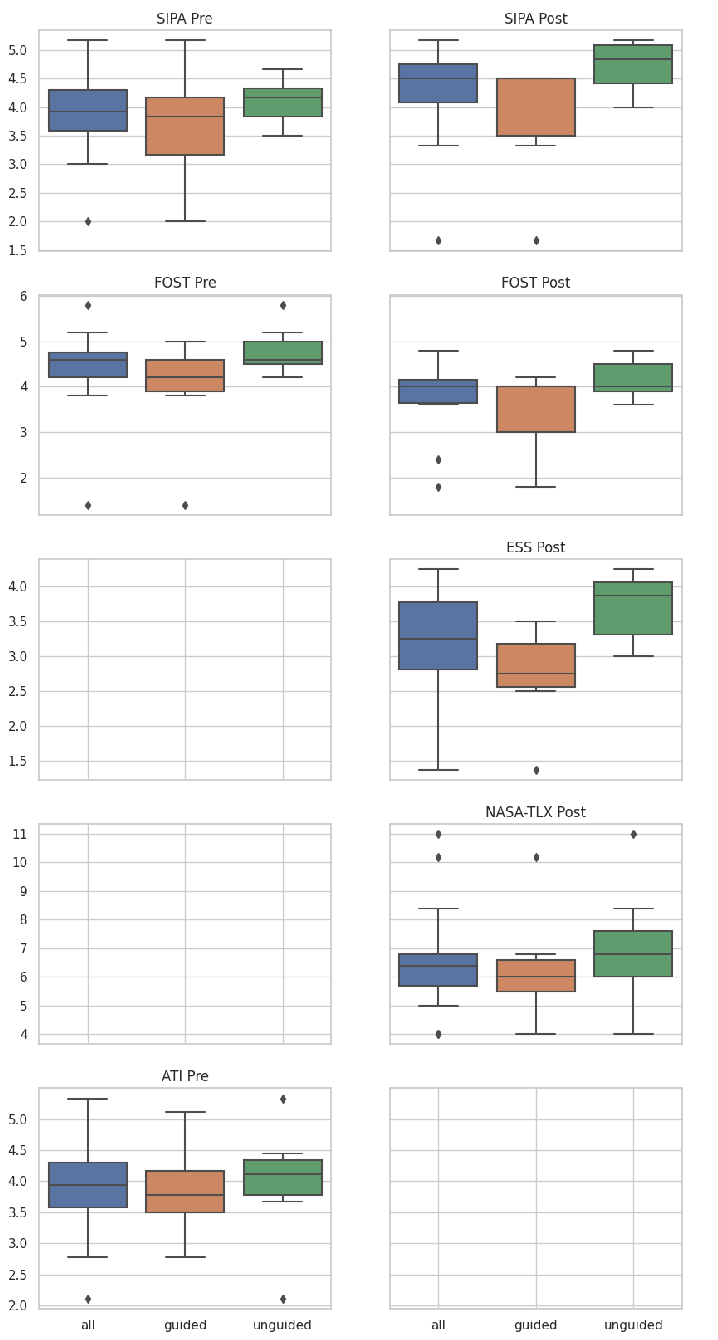
\includegraphics[width=0.9\textwidth]{img/figures/boxplots.png}
    \caption{Boxplots of Questionnaire Results}
    \label{fig:evaluation_descriptive_boxplots}
\end{figure}

\begin{table}[htbp]
    \centering
    \begin{tabularx}{0.7\textwidth}{ l c c c c c c }
        \toprule
        & \textit{SS} & \textit{df} & \textit{MS} & \textit{F} & \textit{p} & ${\eta^2}_p$ \\
        \midrule
        Time & 1.016 & 1 & 1.016 & 5.41 & .038* & .311 \\
        Time $\ast$ Guidance & 0.397 & 1 & 0.397 & 2.11 & .172 & .150 \\
        Residual & 2.254 & 12 & 0.188 & & & \\
        \bottomrule
        \multicolumn{3}{l}{\footnotesize * $\textit{p}<.05$, ** $\textit{p}<.01$, *** $\textit{p}<.001$} \\
    \end{tabularx}
    \caption{ANOVA - Within Subjects Effects on SIPA}
    \label{table:anova_within_sipa}
\end{table}

\begin{table}[htbp]
    \centering
    \begin{tabularx}{0.6\textwidth}{ l c c c c c c }
        \toprule
        & \textit{SS} & \textit{df} & \textit{MS} & \textit{F} & \textit{p} & ${\eta^2}_p$ \\
        \midrule
        Guidance & 3.11 & 1 & 3.11 & 2.90 & .114 & .195 \\
        Residual & 12.86 & 12 & 1.07 & & & \\
        \bottomrule
    \end{tabularx}
    \caption{ANOVA - Between Subjects Effects on SIPA}
    \label{table:anova_between_sipa}
\end{table}

\begin{table}[htbp]
    \centering
    \begin{tabularx}{0.75\textwidth}{ l c c c c c c }
        \toprule
        & \textit{SS} & \textit{df} & \textit{MS} & \textit{F} & \textit{p} & ${\eta^2}_p$ \\
        \midrule
        Time & 2.2857 & 1 & 2.2857 & 6.4516 & .026* & .350 \\
        Time $\ast$ Guidance & 0.0229 & 1 & 0.229 & 0.0645 & .804 & .005 \\
        Residual & 2.254 & 12 & 0.188 & & & \\
        \bottomrule
        \multicolumn{3}{l}{\footnotesize * $\textit{p}<.05$, ** $\textit{p}<.01$, *** $\textit{p}<.001$} \\
    \end{tabularx}
    \caption{ANOVA - Within Subjects Effects on Trust}
    \label{table:anova_within_trust}
\end{table}

\begin{table}[htbp]
    \centering
    \begin{tabularx}{0.6\textwidth}{ l c c c c c c }
        \toprule
        & \textit{SS} & \textit{df} & \textit{MS} & \textit{F} & \textit{p} & ${\eta^2}_p$ \\
        \midrule
        Guidance & 4.48 & 1 & 4.48 & 4.24 & .062 & .261 \\
        Residual & 12.67 & 12 & 1.07 & & & \\
        \bottomrule
    \end{tabularx}
    \caption{ANOVA - Between Subjects Effects on Trust}
    \label{table:anova_between_trust}
\end{table}

\begin{table}[htbp]
    \centering
    \begin{tabularx}{0.65\textwidth}{ l l c c c }
        \toprule
        & & SIPA (pre) & FOST (pre) & ATI \\
        \midrule
        \multirow[t]{2}{*}{SIPA (pre)} & \textit{r} & --- & & \\
        & \textit{p} & --- & & \\
        \multirow[t]{2}{*}{FOST (pre)} & \textit{r} & .57* & --- & \\
        & \textit{p} & .03 & --- & \\
        \multirow[t]{2}{*}{ATI} & \textit{r} & .13 & -.04 & --- \\
        & \textit{p} & .66 & .89 & --- \\
        \bottomrule
        \multicolumn{5}{l}{\footnotesize * $\textit{p}<.05$, ** $\textit{p}<.01$, *** $\textit{p}<.001$} \\
    \end{tabularx}
    \caption{Correlation Matrix (pre scores)}
    \label{table:correlation_matrix_pre}
\end{table}

\begin{table}[htbp]
    \centering
    \begin{tabularx}{0.9\textwidth}{ l l c c c c c }
        \toprule
        & & ATI & SIPA (post) & FOST (post) & ESS & NASA-TLX \\
        \midrule
        \multirow[t]{2}{*}{ATI} & \textit{r} & --- & & & & \\
        & \textit{p} & --- & & & & \\
        \multirow[t]{2}{*}{SIPA (post)} & \textit{r} & .10 & --- & & & \\
        & \textit{p} & .739 & --- & & & \\
        \multirow[t]{2}{*}{FOST (post)} & \textit{r} & -.02 & .78** & --- & & \\
        & \textit{p} & .94 & $<.01$ & --- & & \\
        \multirow[t]{2}{*}{ESS} & \textit{r} & -.03 & .71** & .68** & --- & \\
        & \textit{p} & .91 & $<.01$ & $<.01$ & --- & \\
        \multirow[t]{2}{*}{NASA-TLX} & \textit{r} & .50 & -.34 & -.38 & -.29 & --- \\
        & \textit{p} & .07 & .23 & .18 & .31 & --- \\
        \bottomrule
        \multicolumn{7}{l}{\footnotesize * $\textit{p}<.05$, ** $\textit{p}<.01$, *** $\textit{p}<.001$} \\
    \end{tabularx}
    \caption{Correlation Matrix (post scores)}
    \label{table:correlation_matrix_post}
\end{table}

\newpage
\section{Conclusion on the Evaluation}
Through a summative evaluation the effects of the implementation on the user could be measured. An on-site experiment study design including within- and between-subject factors delivered statistically significant results. By surveying $\textit{N}=14$ participants with questionnaires such as SIPA, FOST, ESS and NASA-TLX and applying a repeated measure ANOVA, it was discovered how the interaction with an AI assessment system affected explainability and trustworthiness of AI models in the medical context: While SIPA increased, trust decreased. Additionally the correlation between these two variables increased through the interaction. However, the differentiation between guided and unguided interaction did not yield statistically significant results. The subjective workload and the explanation satisfaction was measured to be higher for the unguided group and the explanation satisfaction was correlated with SIPA. 

\newpage
\chapter{Discussion}
The following sections give a summarized overview of the thesis, its results implications and limitations, while also discussing directions for further research.

\section{Summary of Results}
The goal of the thesis was to apply human-centered design research on explainability and trustworthiness of black box AI models and therefore explore the effects of XAI on users to shed light on the requirements for modern AI usage in the medical field.

Through the conception, development and evaluation of an AI assessment system in cooperation with Clearbox, suitable explanation methods were found to impact the perceived understandability and trustworthiness of AI models for the user group of medical professionals. By studying literature and conducting expert interviews (see \autoref{chapter:analysis}) requirements, functionalities, interaction- and interface designs for an interactive AI assessment system were conceptualized (see \autoref{chapter:conception}). Based on the conception, a functional, browser-based prototype was implemented with Streamlit \parencite{streamlit_website} in order to accommodate a flexible usage scenario (see \autoref{chapter:implementation}). By leveraging an open access AI model and data set, the implementation depicts a possible application scenario for the medical domain. Following the human-centered development process, a summative evaluation of the prototype with $\textit{N}=14$ participants was conducted. The evaluation consisted of an on-site experiment with medical students including within- and between-subject factors. Analysing the evaluation results yielded insights into the effects of the HCI in both subject groups (see \autoref{chapter:evaluation}).

The statistical analysis of the evaluation results showed, that the interaction with the assessment system had a significant effect on the subjective understandability and the perceived trustworthiness of the AI model. However, the effects go the opposite way: Understandability increased through the interaction, but trustworthiness decreased. This is a interesting finding, because it highlights a particular effect on users: Through better subjective understanding, the user's trust in the model was possibly calibrated and the user perceived the model as less trustworthy. Remarkably, the SIPA and FOST pre-test scores, which are based only on the textual explanation of the evaluation questionnaire (see \nameref{appendix:evaluation_questionnaire}), were already quite high.

Comparing the between-subject effects, no statistical significance was found. However, the guided group showed a tendency towards smaller effect size on subjective understandability and trust, compared to the unguided group. This leads to the question, whether an open interaction style leads to a higher perceived feeling of understandability. \textcite{sedig_role_2001} already explored the effects of scaffolding on cognition in learnware, and found that HCI artifacts can extend or, inadvertently, limit human cognition and thought processes. There seems to be a connection between the cognitive load in a learning context and the between-subject effects observed in this evaluation. However, because of the missing significance, the effects of guidance and scaffolding in XAI should be further studied with a focus on the distinction between content-related versus non-content-related aspects of the GUI as proposed by \textcite{sedig_role_2001}.

Also the perceived workload was overall higher in the unguided group compared to the guided group. This indicates that the guidance helped with workload, even though it does not correlate with neither SIPA or trust. However, no meaningful measure of objective workload could be observed. A higher perceived workload in the unguided group, combined with the tendency towards a stronger effect on SIPA and trust, might indicate similar psychological effects as described in the \textit{Elaboration Likelihood Model} by \textcite{petty_elaboration_1986}: The stronger effects on subjective understandability and trust in the unguided group suggest information processing via the central route, which consumes more cognitive resources and is in line with the higher perceived workload. Additionally, when the user processes the presented information through the central route a higher need for cognition is to be expected. If one takes the the rather high ATI score of the participants into consideration, a connection between a higher need for cognition and a stronger effect on SIPA and trust is possible and invites to further research.

While it is not possible to discriminate the effects of each explanation method used by the summative evaluation design, the explanation satisfaction and the SIPA post-test score are also correlated. The display of structured meta data in addition to the image data was part of most explanation methods (and the main focus of one method). The within-subject effect on SIPA leads to the assumption that the presentation of meta data does increase the user's subjective understanding of the AI model's operational range and performance. Referencing the qualitative data, many participants even whished for more meta data, such as clinical data of the patient, which supports a connection between meta data presentation and explanation satisfaction.

Interestingly ATI, a key facet of user personality, does not have any correlation with the other variables. Seemingly the tendency to actively engage in intensive technology interaction has no effects on the information reception of the user, as neither SIPA or trust are correlated with it. Although the small sample size, only consisting of young medical students with relatively high ATI scores, may distort this finding.

\section{Implications}
The within-subject effects support the answer of the research questions Q1 \& Q2: For this AI model and data set, SIPA and trust are correlated. Additionally the correlation increased through the interaction with the assessment system. Therefore the presented functionalities and explanation methods are suitable to increase understanding and possibly optimize the trust levels through the interaction. By supplementing the qualitative data, especially the the input-output experiment and the data browsing functionality were beneficial to the moderate SIPA and trust. On the other hand, the visual explanation was controversially perceived and might not be suitable to explain an AI model to medical professionals. Furthermore the qualitative data shows, that participants from this sample want more technical details about image classifiers.

With the limitation of the missing discrimination of the explanation methods used, research question Q4 can also be answered by the within-subject effects on SIPA: The presentation of meta data in the assessment system is part of the explanation methods used and therefore involved in the significant increase in perceived understandability of the user.

Because of the inconclusiveness of the between-subject ANOVA, research question Q3 cannot be clearly answered: Stronger effects in the unguided group only suggest, that scaffolding and guidance can impede the perceived understandability and therefore the adaption of trust levels. A free, explorative interaction method therefore may be beneficial to understandability and trust.  

\section{Limitations}
Originally a more diverse user group was depicted, including medical professionals and data scientists. Already in the user analysis (see \autoref{section:user_analysis}) first issues emerged regarding the quantity of information to be gathered on the user group of data scientists. During the further conception this lack of information led to a strong focus on the user group of medical professionals. The focus was maintained until the summative evaluation, where it culminated in a homogeneous medical participant group. Because of the inherent differences between the user groups, the results are only meaningful for medical professionals. Even then, the participants surveyed belonged to a limited demographic, leading to a more difficult generalizability of the results. Additionally the small sample size might negatively influence the results of the variance analysis.

Furthermore this study only observes the effects of XAI on users for a particular image classifier. Therefore a generalization on other medical application domains, such as symptomatic diagnostics cannot be made.

\section{Further Research}
The inconclusive results on the comparison between guided and unguided interaction only allowed for assumptions regarding the effects of guidance on understandability and trustworthiness. However this can be a great starting point for further research, focusing on the concrete mode of HCI in the XAI context. By developing user interfaces and interactive explanation methods with specialized frontend technologies, the intricacies of guidance and scaffolding for human-AI-interaction could be further explored. Additionally many other feasible explanation methods, such as the omitted comparative explanations or different visual explanations could be implemented and the effects on the users studied. Complemented with a more diverse participant group and additional measures for explainability and trustworthiness, the presented results can be used as a foundation for a further research on HCI in the XAI context.

\newpage
\chapter{Conclusion}
With the all pervasive use of artificial intelligence in current technological advances, the XAI research domain grows ever since. The goal of the thesis was to design and develop an human-centered AI assessment system to make an AI model more explainable and thus facilitate understandability and trustworthiness for the user. Leveraging the knowledge of the HCI domain and combining it with current XAI literature, tools and research partners has resulted in conceptualizing, implementing and evaluating a functional AI assessment system prototype for the context of medical applications. Considering the potential user's needs and requirements throughout the entire development process is an important part of human-centered application development. Expert interviews gave insights into the needs and requirements of the potential users of an AI model in the medical context. Based on these requirements and XAI literature, functionalities, explanation methods, interaction- and interface design were conceptualized and implemented with a strong focus on understandability and coactive HCI. The functional prototype was then evaluated in a study with medical students. The evaluation's results depict connections between interactive explanations, understandability and trustworthiness of AI models. A summative evaluation of a AI assessment system prototype showed that the user's subjective understanding of the AI model increased through the interaction with said system. Furthermore the user's trust has decreased through the interaction with the system for the specific AI model used. Therefore interactive explanation methods, such as (1) contextual train data browsing (2) showing model limitations through false positives and false negatives (3) input-output experiments (4) visual explanation by attribution through occlusion are suitable for moderating the user's subjective understanding and perceived trustworthiness of an AI model. In addition it was found that guidance in the HCI reduced the explanation satisfaction, while showing no significant effects on understandability and trust for the users sampled. However, the results give insights into the complex concepts of understandability and trustworthiness for human-AI-interaction in the medical context and create a foundation for further research.

\clearpage
\phantomsection
\addcontentsline{toc}{chapter}{Abbildungsverzeichnis}
\listoffigures
\clearpage

\phantomsection
\addcontentsline{toc}{chapter}{Tabellenverzeichnis}
\listoftables
\clearpage

\phantomsection
\addcontentsline{toc}{chapter}{Quellen}
\chapter*{Quellen}

\phantomsection
\printbibliography[heading=subbibintoc, nottype=online, nottype=software]

\phantomsection
\printbibliography[heading=subbibintoc, type=online, title=Websites]
\begin{comment}
Websites haben nicht die gleiche Fundierung/Überzeugungskraft wie wissenschaftliche Literatur (peer-review/Anspruch). Die Websites separat aufzuführen, macht es einfacher zu sehen, was wirklich wissenschaftlich fundierte Literatur ist.
\end{comment}

\phantomsection
\printbibliography[heading=subbibintoc, type=software, title=Software]
\begin{comment}
Software-Name mit Versionsnummer und Link zur Website. Nur was für die konkrete Arbeit relevant ist. Das Sie die Arbeit mit Word geschrieben haben, ist irrelevant. Das sieht man. LaTeX auch.
\end{comment}
\clearpage

\phantomsection
\addcontentsline{toc}{chapter}{Abkürzungen}
\chapter*{Abkürzungen}
\begin{comment}
Kann recht kurz ausfallen, aber falls Sie bestimmte Abkürzungen häufiger verwenden, hier aufführen. Geht nur darum, dass der Leser hierhin blättern könnte, wenn er über eine unbekannte Abkürzung stolpert. Ist beim digitalen Lesen hinfällig geworden. Hier geht es wirklich nur um Akronyme, z. B. ICBM = Intercontinental Ballistic Missile, oder PIN = Personal Identification Number. Die Erläuterung von Begriffen erfolgt im Glossar.
\end{comment}

\begin{description}
    \item [\textbf{Akronym}] Ausgeschriebenes Akronym
\end{description}
\clearpage

\phantomsection
\addcontentsline{toc}{chapter}{Glossar}
\chapter*{Glossar}
\begin{comment}
Unterschiedliche Disziplinen verwenden z. T. die selben Begriffe für unterschiedliche Sachverhalte und unterschiedliche Begriffe für die selben Sachverhalte. Hier können Sie wiederkehrende zentrale Begriffe der Arbeit kurz definieren (z. B. Adipositas, Depression, Legasthenie, etc.). Früher wichtiger, dann konnte man hierhin blättern und musste nicht den ganzen Text absuchen. Heute verwendet man digital die Suchfunktion. Trotzdem ernst nehmen.
\end{comment}

\begin{description}
    \item [\textbf{Begriff}] Kurze Erläuterung
\end{description}
\clearpage

\phantomsection
\addcontentsline{toc}{chapter}{Anhänge}
\chapter*{Anhänge}
\begin{comment}
Zusätzliche Informationen die zu lang für die Arbeit sind können hier verfügbar gemacht werden.

Aber auch an die DVD denken — was ist dort besser aufgehoben? Die Zeiten, in denen man Programmcode manuell eingetippt hat, sind ja glücklicherweise lange vorbei, deswegen macht Code hier wenig Sinn.

Ist entsprechend ein Priorisierung: Was würde sich der Leser vielleicht gerne während des Lesens der Arbeit (z. B. im Zug) ansehen, wenn er auch gerade nicht auf die DVD zugreifen kann (kein DVD Laufwerk)?

Inhalte sind oft: Überblick der Inhalte der DVD, Fragebögen (falls digital Screenshots oder neu für den Druck formatiert), Interviewleitfäden, etc. Selten detailliertere Evaluationsergebnisse.

Hier kurz die Zwischenüberschriften nennen und evtl. 1 Satz, was dort zu finden ist (falls es nicht schon durch die Zwischenüberschrift klar ist). 
\end{comment}

Text \dots

\phantomsection
\addcontentsline{toc}{section}{Anhang A: Inhalt der DVD}
\section*{Anhang A: Inhalt der DVD}
\begin{comment}
Oft ein Default: Was findet man auf der beiliegenden DVD in welchem Verzeichnis? Max. 1 Seite.

\textbf{In jedem Fall} die PDF der Arbeit, den Programmcode, Daten (anonymisiert!).

\textbf{Niemals} Interviewaufzeichnungen, Einverständniserklärungen oder ähnliche personenbezogene Daten auf die DVD brennen — Sie haben in den meisten Fällen Anonymität zugesichert und die DVD ist frei zugänglich (ein Exemplar der Arbeit kommt in die Bibliothek). 
\end{comment}

Text \dots

\phantomsection
\addcontentsline{toc}{section}{Anhang B: Anhangstitel}
\section*{Anhang B: Anhangstitel}
\begin{comment}
Weitere Inhalte je nachdem, wo der Leser ohne großen Aufwand hinspringen sollte.
\end{comment}

Text \dots

\clearpage

\phantomsection
\addcontentsline{toc}{chapter}{Erklärung}
\chapter*{Erklärung}
Ich versichere an Eides statt, die vorliegende Arbeit selbstständig verfasst und nur die angegebenen Quellen benutzt zu haben.

\begin{comment}
[Nach Ausdruck unterschreiben. Muss auf Papier sein.]
\end{comment}

-----------------------------------------------------------------

Lübeck, \today, \authorMA
\end{document}
